% !Mode:: "TeX:UTF-8"
\documentclass{ctexart}
\usepackage{amsmath, amssymb, geometry, ulem, graphicx, diagbox, xcolor, mdframed, tasks, fancyhdr, lastpage, fixdif}

\geometry{a4paper, left=20mm, right=20mm, top=20mm, bottom=20mm}
\fancyhf{}
\pagestyle{fancy}
\fancyfoot[C]{第 \thepage\ 页,共 \pageref{LastPage} 页}
\renewcommand{\headrulewidth}{0pt}

\newcommand{\newpaper}
{
	\newpage
	{\large\noindent\uline{\text{《概率论与数理统计》习题册} \hfill 长江大学信息与数学学院}\\
	班级\uline{测试12345} \hfill 姓名\uline{佚名} \hfill 班内序号\uline{01}}\par
}
\newcommand{\oldpaper}
{
	\newpage
	{\large\noindent\uline{\text{《概率论与数理统计》习题册} \hfill 长江大学信息与数学学院}}\par\noindent
}
\newcommand{\sectionstar}[1]
{
	\section*{#1}
	\addcontentsline{toc}{section}{#1}\ignorespaces
}
\newcommand{\shortlabel}[1]
{
	\hfill
	{\small(#1)}\ignorespaces
}
\newcommand{\longlabel}[1]
{
	\\
	\hspace*{0mm}
	\hfill
	{\small(#1)}\ignorespaces
}
\newcommand{\highlightbox}[1]
{\fcolorbox{black}{gray!40}{$#1$}}
\newcommand{\mfrac}[2]{\scalebox{0.8}{$\dfrac{#1}{#2}$}}

\newcounter{problemcounter}
\makeatletter
\@addtoreset{problemcounter}{section}
\makeatother

\newenvironment{problem}
{
	\stepcounter{problemcounter}
	\begin{mdframed}[backgroundcolor=gray!40, hidealllines=true]
	\theproblemcounter.\ignorespaces
}
{  
	\end{mdframed}
}
\newenvironment{solution}
{
	\noindent 解:\ignorespaces
}
{
}
\newenvironment{answer}
{
	\begin{mdframed}[backgroundcolor=gray!40, hidealllines=true, skipabove=0pt, skipbelow=0pt]
	\noindent\ignorespaces
}
{  
	\end{mdframed}
}

\NewTasksEnvironment[
label = (\Alph*), 
label-width = 1.5em, 
item-indent = 2em 
]{mytasks}[\task](2) 

\begin{document}
\thispagestyle{empty}
\tableofcontents
\thispagestyle{empty}
\newpaper
\setcounter{page}{1}
\section{样本空间、随机事件、概率}
\noindent 一、填空题.\\ 1.设$A,B,C$为三事件,用$A,B,C$的运算关系表示下列各事件.\\
(1)$A$发生,$B$与$C$不发生:\uline{$A\overline{B}\,\overline{C}$}\\
(2)$A$与$B$都发生,而$C$不发生:\uline{$AB\overline{C}$}\\
(3)$A,B,C$中至少有一个发生:\uline{$A\bigcup B\bigcup C$}\\
(4)$A,B,C$都不发生:\uline{$\overline{A}\,\overline{B}\,\overline{C}$}\\
(5)$A,B,C$中不多于一个发生:\uline{$(\overline{A}\,\overline{B})\bigcup(\overline{A}\,\overline{C})\bigcup(\overline{B}\,\overline{C})$}\\
(6)$A,B,C$中不多于两个发生:\uline{$\overline{ABC}$}\\
(7)$A,B,C$中至少有两个发生:\uline{$(AB)\bigcup(AC)\bigcup(BC)$}\\ 2.设$A,B$为两随机事件且$P(AB)=\dfrac{3}{7}$,$P(A)=P(B)=\dfrac{4}{7}$,则$P(A\bigcup B)=\uline{\dfrac{5}{7}}$\\ 
3.设$A\supset B$,$P(A)=p$,$P(B)=q$,则$P(A-B)=\uline{p-q}$\\ 
4.判断下列命题的正误.\\ %\checkmark or $\times$
(1)$A\bigcup B=(AB)\bigcup B$ ($\times$) \hfill
(2)$\overline{A}B=A\bigcup B$ ($\times$)\\
(3)若$AB=\varnothing$,且$C\subset A$,则$BC=\varnothing$ (\checkmark) \hfill
(4)若$B\subset A$,则$A\bigcup B=A$ (\checkmark)\\
二、计算题.
\begin{problem}
写出下列随机试验的样本空间$\Omega$和下列事件所包含的样本点.\\
(1)掷一颗骰子,出现奇数点;\\
(2)掷两颗骰子,$A=$“出现点数之和为奇数,且恰好其中有一个1点”.
\end{problem}
\begin{solution}
(1)样本空间$\Omega=\{1,2,3,4,5,6\}$,事件$E=\{1,3,5\}$;\\
(2)样本空间$\Omega=\{(1,1)(1,2)(1,3)(1,4)(1,5)(1,6)(2,1)(2,2)(2,3)(2,4)(2,5)(2,6)(3,1)(3,2)(3,3)(3,4)\\(3,5)(3,6)(4,1)(4,2)(4,3)(4,4)(4,5)(4,6)(5,1)(5,2)(5,3)(5,4)(5,5)(5,6)(6,1)(6,2)(6,3)(6,4)(6,5)(6,6)\}$,\\事件$A=\{(1,2)(1,4)(1,6)(2,1)(4,1)(6,1)\}$
\end{solution}
\begin{problem}
设$A,B$为两事件且$P(A)=0.6$,$P(B)=0.7$,问\\
(1)在什么条件下$P(AB)$取到最大值,最大值是多少?\\
(2)在什么条件下$P(AB)$取到最小值,最小值是多少?
\end{problem}
\begin{solution}(1)当$A\subset B$时,此时$P(AB)=0.6$;\\
(2)$P(A\bigcup B)=P(A)+P(B)-P(AB)\le 1$,故$P(AB)\ge 0.3$,当$P(A\bigcup B)=1$时取等
\end{solution}
\begin{problem}
设$A,B,C$为三事件,且$P(A)=P(B)=P(C)=\dfrac{1}{4}$,$P(AB)=P(BC)=0$,$P(AC)=\dfrac{1}{8}$,求$A,B,C$至少有一个发生的概率.
\end{problem}
\begin{solution}
$P(A\bigcup B\bigcup C)=P(A)+P(B)+P(C)-P(AB)-P(AC)-P(BC)+P(ABC)=\dfrac{5}{8}$
\end{solution}
\begin{problem}
设$A,B$为两事件,且$P(A)=0.7$,$P(A-B)=0.3$,求$P(\overline{AB})$.
\end{problem}
\begin{solution}
由于$P(A)=P(A\bigcap S)=P(A\bigcap(B\bigcup\overline{B}))=P(AB\bigcup A\overline{B})=P(AB)+P(A\overline{B})$,由题意得$P(A-B)=P(A\overline{B})=0.3$,于是$P(AB)=0.4$,故$P(\overline{AB})=1-P(AB)=0.6$
\end{solution}
\newpaper
\section{古典概型}
\noindent 一、填空题.\\
 1.已知6只产品中有两只次品,在其中任取两只,则两只都是正品的概率是$\uline{\dfrac{2}{5}}\left(\dfrac{C^{2}_{4}}{C^{2}_{6}}\right)$\\
2.设一同学书桌上放着9本书,其中有3本英语书,现随机取两本,取到的全是英语书的概率为$\uline{\dfrac{1}{12}}\left(\dfrac{C^{2}_{3}}{C^{2}_{9}}\right)$\\
3$^*$.在11张卡片上分别写上probability这11个字母,从中任意连续抽取7张进行排列,则排列结果为ability的概率为$\uline{\dfrac{4}{A^{7}_{11}}}$\\
二、计算题.
\begin{problem}
对一个5人小组考虑生日问题:\\
(1)求5个人的生日都在星期日的概率;\\
(2)求5个人的生日都不在星期日的概率;\\
(3)求5个人的生日不都在星期日的概率.
\end{problem}
\begin{solution}
(1)记事件$A$:5个人的生日都在星期日,5个人一共有$7^5$种可能,于是$P(A)=\dfrac{1}{7^5}$;\\
(2)记事件$B$:5个人的生日都不在星期日,即生日都在前6天,于是$P(B)=\dfrac{6^5}{7^5}$;\\
(3)$P(\overline{A})=1-P(A)=1-\dfrac{1}{7^5}$
\end{solution}
\begin{problem}
从52张扑克牌中任意取出13张,问有5张黑桃,3张红心,3张方块,2张梅花的概率是多少?
\end{problem}
\begin{solution}
$P=\dfrac{C^{5}_{13}C^{3}_{13}C^{3}_{13}C^{2}_{13}}{C^{13}_{52}}$
\end{solution}
\begin{problem}
在房间里有10个人,分别佩戴从1号到10号的纪念章,任选3人记录其纪念章的号码,求\\
(1)最小号码为5的概率;(2)最大号码为5的概率.
\end{problem}
\begin{solution}
(1)最小号码为5,即从比5大的5个号码中选2个,于是$P_1=\dfrac{C^{2}_{5}}{C^{3}_{10}}=\dfrac{1}{12}$;\\
(2)最大号码为5,即从比5小的4个号码中选2个,于是$P_2=\dfrac{C^{2}_{4}}{C^{3}_{10}}=\dfrac{1}{20}$
\end{solution}
\begin{problem}
随机地向半圆$0<y<\sqrt{2ax-x^2}$($a$为正常数)内掷一点,点落在半圆内任何区域的概率与区域的面积成正比,则原点和该点的连线与$x$轴的夹角小于$\dfrac{\pi}{4}$的概率是多少?
\end{problem}
\begin{solution}
\begin{minipage}[t]{0.7\textwidth}
作图可知$P=\dfrac{\dfrac{\pi a^2}{4}+\dfrac{a^2}{2}}{\dfrac{\pi a^2}{2}}=\dfrac{1}{2}+\dfrac{1}{\pi}$
\end{minipage}
\hfill
\begin{minipage}[t]{0.25\textwidth}
\centering
\raisebox{-0.5\height}{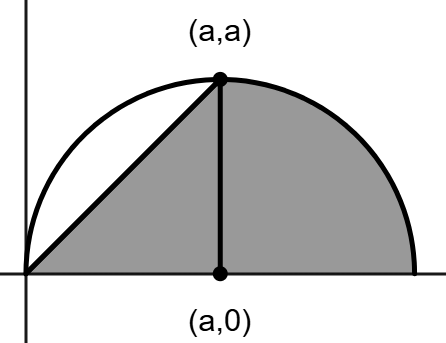
\includegraphics[width=\linewidth]{2.4.png}}  
\end{minipage}
\end{solution}
\newpaper
\section{条件概率、全概率公式}
\noindent 一、计算题.
\begin{problem}
设$P(\overline{A})=0.3$,$P(B)=0.4$,$P(A\overline{B})=0.5$,求$P(B\mid A\bigcup\overline{B})$.
\end{problem}
\begin{solution}
$P(A)=1-P(\overline{A})=P(AB)+P(A\overline{B})$,$P(B)=P(BA)+P(B\overline{A})=P(B\mid A\bigcup\overline{B})P(A\bigcup\overline{B})+P(B\mid\overline{A}B)P(\overline{A}B)$,故$P(AB)=0.2$,$P(\overline{A}B)=0.2$,又$P(B\mid\overline{A}B)=1$,则$P(B\mid A\bigcup\overline{B})=0.25$
\end{solution}
\begin{problem}
已知在10只产品中有2只次品,在其中取两次,每次任取一只,作\textbf{不放回抽样},求下列事件的概率:(1)两只都是正品;(2)两只都是次品;(3)一只是正品,一只是次品;(4)第二次取出的是次品.
\end{problem}
\begin{solution}
记事件$A_i$:第$i(i=1,2)$次抽到的是正品,于是\\
(1)$P(A_1A_2)=P(A_1)P(A_2\mid A_1)=\dfrac{8}{10}\times\dfrac{7}{9}=\dfrac{28}{45}$;\\
(2)$P(\overline{A_1}\,\overline{A_2})=P(\overline{A_1})P(\overline{A_2}\mid \overline{A_1})=\dfrac{2}{10}\times\dfrac{1}{9}=\dfrac{1}{45}$;\\
(3)$P(A_1\overline{A_2})+P(\overline{A_1}A_2)=P(A_1)P(\overline{A_2}\mid A_1)+P(\overline{A_1})P(A_2\mid \overline{A_1})=\dfrac{8}{10}\times\dfrac{2}{9}+\dfrac{2}{10}\times\dfrac{8}{9}=\dfrac{16}{45}$;\\
(4)$P(\overline{A_2})=P(A_1\overline{A_2})+P(\overline{A_1}\,\overline{A_2})=\dfrac{1}{5}$
\end{solution}
\begin{problem}
某人忘记了电话号码的最后一个数字,因而他随意地拨号,问:他拨号不超过3次而接通所需电话的概率;若已知最后一个数字是奇数,那么此概率是多少?
\end{problem}
\begin{solution}
记事件$A_i$:第$i(i=1,2,3)$次接通,于是
$P(A_1\bigcup\overline{A_1}A_2\bigcup\overline{A_1}\,\overline{A_2}A_3)=P(A_1)+P(\overline{A_1}A_2)+P(\overline{A_1}\,\overline{A_2}A_3)=\dfrac{1}{10}+\dfrac{9}{10}\times\dfrac{1}{9}+\dfrac{9}{10}\times\dfrac{8}{9}\times\dfrac{1}{8}=\dfrac{3}{10}$,若最后一个数字是奇数,$P(A_1\bigcup\overline{A_1}A_2\bigcup\overline{A_1}\,\overline{A_2}A_3)=P(A_1)+P(\overline{A_1}A_2)+P(\overline{A_1}\,\overline{A_2}A_3)=\dfrac{1}{5}+\dfrac{4}{5}\times\dfrac{1}{4}+\dfrac{4}{5}\times\dfrac{3}{4}\times\dfrac{1}{3}=\dfrac{3}{5}$
\end{solution}
\begin{problem}
已知男子有5\%是色盲患者,女子有0.25\%是色盲患者.今从男女人数相等的人群中随机地挑选一人,恰好是色盲患者,问此人是男性的概率是多少?
\end{problem}
\begin{solution}
记事件$A$:此人是男性,事件$B$:此人是女性,事件$E$:此人是色盲,于是\\
$P(A\mid E)=\dfrac{P(E\mid A)P(A)}{P(E\mid A)P(A)+P(E\mid B)P(B)}=\dfrac{5\%\times0.5}{5\%\times0.5+0.25\%\times0.5}=\dfrac{20}{21}$
\end{solution}
\begin{problem}
有两箱同种类的零件.第一箱装50只,其中10只一等品;第二箱装30只,其中18只一等品.今从两箱中挑选出一箱,然后从该箱中取零件两次,每次任取1只,作不放回抽样.求:(1)第一次取到的零件是一等品的概率;(2)第一次取到的零件是一等品的条件下,第二次取到的也是一等品的概率.
\end{problem}
\begin{solution}
记事件$A_i$:取到的是第$i(i=1,2)$箱,记事件$B_i$:第$i(i=1,2)$次取到的是一等品,于是\\
(1)$P(B_1)=P(A_1B_1)+P(A_2B_1)=\dfrac{1}{2}\times\dfrac{1}{5}+\dfrac{1}{2}\times\dfrac{3}{5}=\dfrac{2}{5}$;\\
(2)$P(B_2\mid B_1)=\dfrac{P(A_1B_1B_2)+P(A_2B_1B_2)}{P(B_1)}=\dfrac{\dfrac{1}{2}\times\dfrac{1}{5}\times\dfrac{9}{49}+\dfrac{1}{2}\times\dfrac{3}{5}\times\dfrac{17}{29}}{\dfrac{1}{2}\times\dfrac{1}{5}+\dfrac{1}{2}\times\dfrac{3}{5}}=\dfrac{690}{1421}$
\end{solution}
\newpaper
\section{独立性}
\noindent 一、填空题.\\ 
1.假设$A,B$是两个相互独立的事件,$P(A\bigcup B)=0.7$,$P(A)=0.3$,则$P(B)=\uline{\dfrac{4}{7}}$\\ 2.某人向同一目标重复射击,每次命中率为$p\left(0<p<1\right)$,则此人第四次射击恰好是第二次命中的概率为$\uline{3p^2(1-p)^2}$\\
二、计算题.
\begin{problem}
三人独立地去破译一份密码,已知各人能译出的概率分别为$\dfrac{1}{5},\dfrac{1}{3},\dfrac{1}{4}$,问三人中至少有一个能将密码译出的概率是多少?
\end{problem}
\begin{solution}
记事件$A_i$:第$i(i=1,2,3)$人破译出,于是
$P(A_1\bigcup A_2\bigcup A_3)=1-P(\overline{A_1}\,\overline{A_2}\,\overline{A_3})=1-\dfrac{4}{5}\times\dfrac{2}{3}\times\dfrac{3}{4}=\dfrac{3}{5}$
\end{solution}
\begin{problem}
袋中装有$m$只正品硬币,$n$只次品硬币(次品硬币的两面均有国徽),在袋中任取一只,将它投掷$r$次,已知每次都得到国徽,问这只硬币是正品的概率是多少?
\end{problem}
\begin{solution}
记事件$A$:取到正品硬币,事件$B$:投掷$r$次得到国徽,于是\\
$P(A\mid B)=\dfrac{P(A)P(B\mid A)}{P(A)P(B\mid A)+P(\overline{A})P(B\mid \overline{A})}=\dfrac{\dfrac{m}{m+n}\times\left(\dfrac{1}{2}\right)^r}{\dfrac{m}{m+n}\times\left(\dfrac{1}{2}\right)^r+\dfrac{n}{m+n}}=\dfrac{m}{m+n\cdot2^r}$
\end{solution}
\begin{problem}
甲、乙、丙3人独立地向飞机射击,设击中的概率分别是$0.4,0.5,0.7$,若只有一人击中,则飞机被击落的概率为0.2;若有两人击中,则飞机被击落的概率为0.6;若三人都击中,则飞机一定被击落,求飞机被击落的概率.
\end{problem}
\begin{solution}记事件$A_i$:飞机被$i(i=1,2,3)$人击中,事件$E$:飞机被击落,于是\\
$P(E)=P(A_1E)+P(A_2E)+P(A_3E)=(0.4\times0.5\times0.3+0.6\times0.5\times0.3+0.6\times0.5\times0.7)\times0.2+(0.4\times0.5\times0.3+0.4\times0.5\times0.7+0.6\times0.5\times0.7)\times0.6+0.4\times0.5\times0.7=0.458$
\end{solution}
\begin{problem}
证明:若$P(A\mid B)=P(A\mid \overline{B})$,则$A,B$相互独立.(提示:$P(A\overline{B})=P(A)-P(AB)$)
\end{problem}
\begin{solution}
因为$P(A\overline{B})=P(A)-P(AB)=P(\overline{B})P(A\mid\overline{B})$,则$P(A)=P(B)P(A\mid B)+P(\overline{B})P(A\mid\overline{B})$,又$P(A\mid B)=P(A\mid \overline{B})$,则$P(A)=(P(B)+P(\overline{B}))P(A\mid B)=P(A\mid B)$,故$P(AB)=P(A)P(B)$,于是$A,B$相互独立
\end{solution}
\newpaper
\section{离散型随机变量及其分布律}
\begin{problem}
一袋中装有5只球,编号为$1,2,3,4,5$,在袋中同时取3只,以$X$表示3只求中的最大号码,写出随机变量$X$的分布律.
\end{problem}
\begin{solution}
$P\left\{X=k\right\}=\dfrac{C^2_{k-1}}{C^3_5}$,$k=3,4,5$
\end{solution}
\begin{problem}
进行重复独立试验,设每次试验成功的概率为$p$,失败的概率为$q=1-p\left(0<p<1\right)$.\\
(1)将试验进行到出现一次成功为止,以$X$表示所需的试验次数,求$X$的
分布律.(此时称$X$服从以$p$为参数的\textbf{几何分布})\\ 
(2)将试验进行到出现$r$次成功为止,以$Y$表示所需的试验次数,求$Y$的
分布律.(此时称$Y$服从以$r,p$为参数的\textbf{巴斯卡分布}) 
\end{problem}
\begin{solution}
(1)$P\left\{X=k\right\}=p(1-p)^{k-1}$,$k=1,2,3,\cdots$;\\
(2)$P\left\{Y=k\right\}=C^{r-1}_{k-1}p^r(1-p)^{r-k}$,$k=r,r+1,r+2,\cdots$
\end{solution}
\begin{problem}
设离散型随机变量$X$的分布律为:$P(X=k)=b\lambda^k,\left(k=1,2,3,\cdots\right)$且$b>0$,求$\lambda$的值.
\end{problem}
\begin{solution}
因为$\displaystyle\sum_{k=1}^{\infty}P\left\{X=k\right\}=\sum_{k=1}^{\infty}b\lambda^k=b\sum_{k=1}^{\infty}\lambda^k=b\cdot\dfrac{\lambda}{1-\lambda}=1$,所以$\lambda=\dfrac{1}{b+1}$
\end{solution}
\begin{problem}
设随机变量$X$服从泊松分布,且满足$P\left\{X=1\right\}=P\left\{X=2\right\}$,求$P\left\{X=4\right\}$.
\end{problem}
\begin{solution}因为$P\left\{X=k\right\}=\dfrac{\lambda^k\mathrm{e}^{-\lambda}}{k!}$,由$P\left\{X=1\right\}=P\left\{X=2\right\}$得$\lambda=2$,则$P\left\{X=4\right\}=\dfrac{2}{3}\mathrm{e}^{-2}$
\end{solution}
\begin{problem}
甲、乙两人投篮,投中的概率分别为$0.6,0.7$,今各投3次,求\\(1)两人投中次数相等的概率;(2)甲比乙投中次数多的概率.
\end{problem}
\begin{solution}
用$X$表示甲投中的次数,$Y$表示乙投中的次数,可知均服从二项分布,则$P\left\{X=k\right\}=C^k_3(0.6)^k(0.4)^{3-k}$,$P\left\{Y=k\right\}=C^k_3(0.7)^k(0.3)^{3-k}$,于是\\
(1)$\displaystyle P\left\{X=Y\right\}=\sum_{k=0}^{3}P\left\{X=k\bigcap Y=k\right\}=\sum_{k=0}^{3}P\left\{X=k\right\}P\left\{Y=k\right\}=\dfrac{8019}{25000}$\\
(2)$\displaystyle P\left\{X>Y\right\}=P\left\{X=1\bigcap Y=0\right\}+P\left\{X=2\bigcap\left\{\bigcup_{k=0}^{1}Y=k\right\}\right\}+P\left\{X=3\bigcap\left\{\bigcup_{k=0}^{2}Y=k\right\}\right\}=P\left\{Y=0\right\}\sum_{k=1}^{3}P\left\{X=k\right\}+P\left\{Y=1\right\}\sum_{k=2}^{3}P\left\{X=k\right\}+P\left\{Y=2\right\}P\left\{X=3\right\}=0.243$
\end{solution}
\newpaper
\section{分布函数与连续型随机变量(一)}
\begin{problem}
将一枚硬币连抛2次,以$X$表示正面朝上的次数,写出$X$的分布律和分布函数,并画出分布函数的图形.
\end{problem}
\begin{solution}
\begin{minipage}[t]{0.5\textwidth}
$P\left\{X=k\right\}=C^k_2\left(\dfrac{1}{2}\right)^2,k=0,1,2$\\
分布函数$F(x)=
\begin{cases} 
	0, &x<0\\ 
	\mfrac{1}{4}, &0\le x<1\\
	\mfrac{3}{4}, &1\le x<2\\
	1, &x\ge2
\end{cases}$
\end{minipage}
\hfill
\begin{minipage}[t]{0.45\textwidth}
	\vspace{0pt}  
	\centering
	\raisebox{-0.5\height}{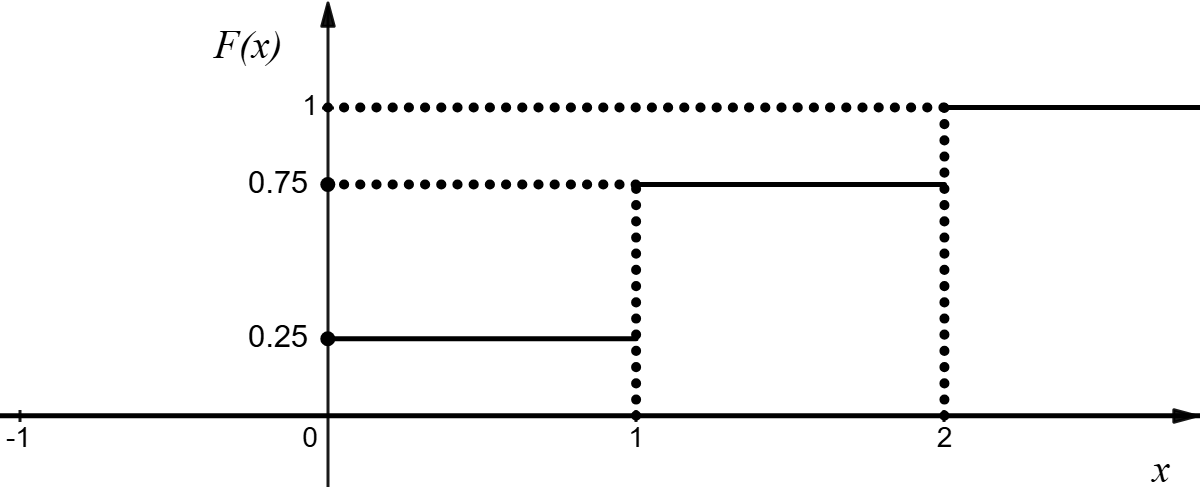
\includegraphics[width=\linewidth]{6.1.png}}  
\end{minipage}
\end{solution}
\begin{problem}
以$X$表示某商店从早晨开始营业起到直到第一个顾客到达的等待时间
(以分钟计),$X$的分布函数是$F_X(x) = 
\begin{cases} 
	1 - \mathrm{e}^{-0.4x}, &x>0\\ 
	0, &x\le0 
\end{cases}$,求下述概率:(1)$P\left\{\text{至多3分钟}\right\}$;(2)$P\left\{\text{至少4分钟}\right\}$;(3)$P\left\{\text{3分钟至4分钟之间}\right\}$;(4)$P\left\{\text{至多3分钟或至少4分钟}\right\}$;(5)$P\left\{\text{恰好2.5分钟}\right\}$.
\end{problem}
\begin{solution}
(1)$P\left\{X\le 3\right\}=F_X(3)=1-\mathrm{e}^{-1.2}$;(2)$P\left\{X\ge 4\right\}=1-P\left\{X<4\right\}=\mathrm{e}^{-1.6}$;
(3)$P\left\{3<x<4\right\}=F_X(4)-F_X(3)=\mathrm{e}^{-1.2}-\mathrm{e}^{-1.6}$;
(4)$P\left\{X\le3\bigcup X\ge4\right\}=1-\mathrm{e}^{-1.2}+\mathrm{e}^{-1.6}$;
(5)$P\left\{X=2.5\right\}=0$
\end{solution}
\begin{problem}
设连续型随机变量$X$的分布函数为:
$$
F(x)=
\begin{cases} 
	A+B\mathrm{e}^{-\lambda x}, &x\ge0\\ 
	0, &x<0 
\end{cases},(\lambda>0)
$$
(1)求常数$A,B$;(2)求$P\left\{X\le 2\right\}$,$P\left\{X>3\right\}$;(3)求密度函数$f(x)$.
\end{problem}
\begin{solution}
(1)由分布函数的性质得$\displaystyle\lim_{x \to +\infty} F(x)=A=1$,$\displaystyle\lim_{x \to 0^-} F(x)=\lim_{x \to 0^+} F(x)=A+B=0\Rightarrow B=-1$;\\
(2)$P\left\{X\le2\right\}=F(2)=1-\mathrm{e}^{-2\lambda}$,$P\left\{X>3\right\}=1-P\left\{X\le3\right\}=\mathrm{e}^{-3\lambda}$;\\
(3)$f(x)=F'(x)=
\begin{cases} 
	\lambda\mathrm{e}^{-\lambda x}, &x\ge0\\ 
	0, &x<0 
\end{cases},(\lambda>0)$
\end{solution}
\begin{problem}
已知随机变量$X$的密度函数为:
$$
f(x)=A\mathrm{e}^{-\left | x \right | },(-\infty<x<+\infty)
$$
求:(1)常数$A$的值;(2)$P\left\{0<X<1\right\}$:(3)$F(x)$.
\end{problem}
\begin{solution}
(1)$\displaystyle\int_{-\infty}^{+\infty}f(x)\d x=\int_{-\infty}^{0}A\mathrm{e}^x\d x+\int_{0}^{+\infty}A\mathrm{e}^{-x}\d x=2A=1$,于是$A=\dfrac{1}{2}$;\\
(2)$\displaystyle P\left\{0<x<1\right\}=\int_{0}^{1}f(x)\d x=\dfrac{1}{2}(1-\mathrm{e}^{-1})$;\\
(3)当$x<0$时,$\displaystyle F(x)=\int_{-\infty}^{x}A\mathrm{e}^t\d t=\dfrac{1}{2}\mathrm{e}^x$;
当$x\ge0$时,$\displaystyle F(x)=\int_{-\infty}^{0}A\mathrm{e}^t\d t+\int_{0}^{x}A\mathrm{e}^{-t}\d t=1-\dfrac{1}{2}\mathrm{e}^{-x}$.于是$F(x)=
\begin{cases} 
	1-\dfrac{1}{2}\mathrm{e}^{-x}, &x\ge0\\
	\dfrac{1}{2}\mathrm{e}^x, &x<0 
\end{cases}$
\end{solution}
\newpaper
\section{连续型随机变量(二)}
\noindent 一、填空题.\\
1.设随机变量$X$服从指数分布,其密度函数为$f(x)=
\begin{cases}
	\mathrm{e}^{-x}, &x>0\\
	0, &x\le0
\end{cases}$,
含有变量$a$的二次方程$a^2+2a+X=0$有实根的概率为$\uline{1-\mathrm{e}^{-1}}$\\ 
2.记$z_\alpha$为标准正态分布随机变量的上$\alpha$分位点,则$z_{0.01}=\uline{2.33}$,$z_{0.003}=\uline{2.75}$,$z_{0.997}=\uline{-2.75}$\\
二、计算题.
\begin{problem}
某种型号的器件的寿命$X$(以小时计)具有以下的概率密度:
$$
f(x)=
\begin{cases}
	\dfrac{1000}{x^2}, &x>1000\\
	0, &\text{其它}
\end{cases}
$$
现有一大批此种器件(设各器件损坏是否相互独立),任取5只,问其中至
少有一只寿命大于1500小时的概率是多少?
\end{problem}
\begin{solution}
$\displaystyle P\left\{X\le1500\right\}=\int_{1000}^{1500}\dfrac{1000}{x^2}\d x=\dfrac{1}{3}$,至少有一只大于的反面即均小于,于是$P=1-\dfrac{1}{3^5}$
\end{solution}
\begin{problem}
设$X\sim N(3,2^2)$ ,求\\
(1)$P\left\{2<X\le5\right\}$,$P\left\{\left|X\right|>2\right\}$;(2)确定$c$使得$P\left\{X>c\right\}=P\left\{X\le c\right\}$;\\
(3)设$d$满足$P\left\{X>d\right\}\ge0.9$,问$d$至多为多少?
\end{problem}
\begin{solution}
(1)$P\left\{2<X\le5\right\}=P\left\{X<5\right\}-P\left\{X\le2\right\}=\varPhi\left(1\right)-\varPhi\left(-\dfrac{1}{2}\right)=\varPhi(1)+\varPhi\left(\dfrac{1}{2}\right)-1=0.5328$,$P\left\{\left|X\right|>2\right\}=1-P\left\{\left|X\right|\le2\right\}=1-P\left\{-2\le X\le 2\right\}=1-(P\left\{X\le 2\right\}-P\left\{X\le -2\right\})=1+\varPhi\left(-\dfrac{5}{2}\right)-\varPhi\left(-\dfrac{1}{2}\right)=1+\varPhi\left(\dfrac{1}{2}\right)-\varPhi\left(\dfrac{5}{2}\right)=0.6977$;\\
(2)由对称性知$c=\mu=3$;\\
(3)$P\left\{X>d\right\}=1-P\left\{X\le d\right\}=1-\varPhi\left(\dfrac{d-3}{2}\right)\ge0.9$,则$\varPhi\left(\dfrac{3-d}{2}\right)\ge0.9$,查表得$\dfrac{3-d}{2}\ge1.29$,故$d\le0.42$
\end{solution}
\begin{problem}
设随机变量$X$和$Y$均服从正态分布,且$X\sim N(\mu,4^2)$,$Y\sim N(\mu,5^2)$,试比较以下$p_1$和$p_2$的大小.
$$
p_1=P\left\{X\le\mu- 4\right\},p_2=P\left\{Y\ge\mu+5\right\}
$$
\end{problem}
\begin{solution}$p_1=\varPhi(-1)=1-\varPhi(1)$,$p_2=1-P\left\{Y<\mu+5\right\}=1-\varPhi(1)$,于是两者相等
\end{solution}
\begin{problem}
设随机变量$X\sim N(\mu,\sigma^2)$,试问:随着$\sigma$的增大,概率$P\left\{\left |  X-\mu\right |<\sigma\right\}$是如何变化的?
\end{problem}
\begin{solution}$P\left\{\left|X-\mu\right|<\sigma\right\}=P\left\{\mu-\sigma<X<\mu+\sigma\right\}=P\left\{X\le\mu+\sigma\right\}-P\left\{X\le\mu-\sigma\right\}=\varPhi(1)-\varPhi(-1)=2\varPhi(1)-1=0.6826$为定值
\end{solution}
\newpaper
\section{随机变量函数的分布}
\begin{problem}
\noindent 设随机变量$X$的分布律为:
$$
\begin{tabular}{|c|c|c|c|c|c|}
\hline
$X$ & -2 & -1 & 0 & 1 & 2 \\
\hline
$p_k$ & 1/5 & 1/6 & 1/5  & 1/15 & 11/30 \\
\hline
\end{tabular}
$$
求$Y=X^2$的分布律.
\end{problem}
\begin{solution}
$$
\begin{tabular}{|c|c|c|c|}
	\hline
	$Y$ & 0 & 1 & 4\\
	\hline
	$p_k$ & 1/5 & 7/30 & 17/30\\
	\hline
\end{tabular}
$$
\end{solution}
\begin{problem}
设随机变量$X$服从$(0,1)$上均匀分布.\\
(1)求$Y=\mathrm{e}^X$的概率密度;(2)求$Y=-2\ln X$的概率密度,
\end{problem}
\begin{solution}由题意知$f_X(x)=
\begin{cases}
	1, &0<x<1\\
	0, &\text{其它}
\end{cases}$,于是\\
(1)$y=g(x)=\mathrm{e}^x$单调递增,$g(0)=1$,$g(1)=e$,$x=g^{-1}(y)=\ln y$,$x'=\dfrac{1}{y}$,则$f_Y(y)=
\begin{cases}
	\dfrac{1}{y}, &1<y<\mathrm{e}\\
	0, &\text{其它}
\end{cases}$;\\
(2)$y=g(x)=-2\ln x$单调递减,$g(1)=0$,$g(0)=+\infty$,$x=g^{-1}(y)=\mathrm{e}^{-\tfrac{y}{2}}$,$x'=-\dfrac{1}{2}\mathrm{e}^{-\tfrac{y}{2}}$,则$f_Y(y)=
\begin{cases}
	\dfrac{1}{2}\mathrm{e}^{-\tfrac{y}{2}}, &y>0\\
	0, &y\le0
\end{cases}$
\end{solution}
\begin{problem}
设$X\sim N(0,1)$ ,求$Y=\left|X\right|$的概率密度.
\end{problem}
\begin{solution}当$y\ge 0$时,$P\left\{Y\le y\right\}=P\left\{-y\le X \le y\right\}=P\left\{X< y\right\}-P\left\{X<-y\right\}= 2P\left\{X<y\right\}-1$,则$f_Y(y)=2f_X(y)=2\varphi(y)$,则$f_Y(y)=
\begin{cases}
	2\varphi(y), &y\ge0\\
	0, &y<0
\end{cases}
$
\end{solution}
\begin{problem}
设随机变量$X$的概率密度为$f(x)=
\begin{cases}
	\dfrac{2x}{\pi^2}, &0<x<\pi\\
	0, &\text{其它}
\end{cases}$,求$Y=\sin X$的概率密度.
\end{problem}
\begin{solution}由$0<x<\pi$知$0<\sin x\le1$,当$0<y<1$时,$P=\left\{Y\le y\right\}=1-P\left\{\arcsin y\le X\le \pi - \arcsin y\right\}=1+P\left\{X<\arcsin y\right\}-P\left\{X<\pi-\arcsin y\right\}$,则$f_Y(y)=f(\arcsin y)\dfrac{1}{\sqrt{1-y^2}}+f(\pi-\arcsin y)\dfrac{1}{\sqrt{1-y^2}}=\dfrac{2}{\pi\sqrt{1-y^2}}$,于是$f_Y(y)=
\begin{cases}
	\dfrac{2}{\pi\sqrt{1-y^2}}, &0<y<1\\
	0, &\text{其它}	
\end{cases}$
\end{solution}
\newpaper
\begin{problem}
设随机变量$X$服从参数为$\dfrac{1}{2}$的指数分布,证明:$Y=1-\mathrm{e}^{-2X}$在区间$(0,1)$上的均匀分布.
\end{problem}
\begin{solution}
由题意知$X$的概率密度为$f_X(x)=
\begin{cases}
	2\mathrm{e}^{-2x}, &x>0\\
	0, &\text{其它}
\end{cases}$,$y=1-\mathrm{e}^{-2x}$单调递增.当$x=0$时,$y$=0;当$x=+\infty$时,$y=1$.于是$P\left\{Y\le y\right\}=P\left\{X\le-\dfrac{1}{2}\ln(1-y)\right\}$,则$f_Y(y)=f_X(-\dfrac{1}{2}\ln(1-y))\left(-\dfrac{1}{2}\cdot\dfrac{1}{1-y}\right)\\(-1)=1(0<y<1)$,则$f_Y(y)=
\begin{cases}
	1, &0<y<1\\
	0, &\text{其它}
\end{cases}$,
故$Y$为区间$(0,1)$上的均匀分布
\end{solution}
\newpaper
\section{二维随机变量和边缘分布}
\noindent 一、填空题.
\\ 1.设二维随机变量$(X,Y)$的联合分布函数为
$$
F(x,y)=A\left(B+\arctan\dfrac{x}{2}\right)\left(\dfrac{\pi}{2}+\arctan y\right),(x,y)\in \mathbf{R}^2
$$ 则常数$A=\uline{\dfrac{1}{\pi^{2}}}$,$B=\uline{\dfrac{\pi}{2}}$
\\ 2.设二维随机变量$(X,Y)$的联合分布函数为$F(x,y)$,则$P\left\{a<X\le b,Y\le d\right\}=\uline{F(b,d)-F(a,d)}$\\
二、计算题.
\begin{problem}
箱子中装有12只开关,其中2只次品,取两次,每次任取一只,考虑两种试验:(1)放回抽样(2)不放回抽样,我们定义随机变量$X,Y$如下:
$$
X=
\begin{cases}
	0, &\text{若第一次取的是正品}\\
	1, &\text{若第一次取的是次品}
\end{cases}
\,
Y=
\begin{cases}
	0, &\text{若第二次取的是正品}\\
	1, &\text{若第二次取的是次品}
\end{cases}
$$试分别就(1)(2)两种情况,写出$X,Y$的联合分布律.
\end{problem}
\begin{solution}
$$
\text{(1)}
\begin{tabular}{c|cc}
	\diagbox{$Y$}{$X$} & 0 & 1 \\
	\hline
	0 & 25/36 & 5/36 \\
	1 & 5/36 & 1/36 \\
\end{tabular}
\text{;(2)}
\begin{tabular}{c|cc}
	\diagbox{$Y$}{$X$} & 0 & 1 \\
	\hline
	0 & 15/22 & 5/33 \\
	1 & 5/33 & 1/66\\
\end{tabular}
$$
\end{solution}
\begin{problem}
设随机变量$(X,Y)$的概率密度为$f(x,y)=
\begin{cases}
	k(6-x-y), &0<x<2,2<y<4\\
	0, &\text{其它}
\end{cases}$\\
(1)确定常数$k$;(2)求$P\left\{X<1,Y<3\right\}$;(3)求$P\left\{X<1.5\right\}$;(4)求$P\left\{X+Y\le 4\right\}$.
\end{problem}
\begin{solution}(1)$\displaystyle \int_{2}^{4}\int_{0}^{2}k(6-x-y)\d x\d y=8k=1\Rightarrow k=\dfrac{1}{8}$;\\
(2)$\displaystyle P\left\{X<1,Y<3\right\}=\int_{2}^{3}\int_{0}^{1}\dfrac{1}{8}(6-x-y)\d x\d y=\dfrac{3}{8}$;\\
(3)$\displaystyle P\left\{X<1.5\right\}=\int_{2}^{4}\int_{0}^{1.5}\dfrac{1}{8}(6-x-y)\d x\d y=\dfrac{27}{32}$;\\
(4)$\displaystyle P\left\{X+Y\le4\right\}=\int_{2}^{4}\int_{0}^{4-y}\dfrac{1}{8}(6-x-y)\d x\d y=\dfrac{2}{3}$
\end{solution}
\begin{problem}
设随机变量$(X,Y)$的概率密度为$f(x,y)=
\begin{cases}
	\mathrm{e}^{-y}, &0<x<y\\
	0, &\text{其它}
\end{cases}$\\
(1)求随机变量的$X$的密度$f_X(x)$;(2)求$\left\{X+Y\le1\right\}$.
\end{problem}
\begin{solution}
(1)当$x>0$时,$\displaystyle f_X(x)=\int_{x}^{+\infty}\mathrm{e}^{-y}\d y=\mathrm{e}^{-x}$,则$f_X(x)=
\begin{cases}
	\mathrm{e}^{-x}, &x>0\\
	0, &x\le0 
\end{cases}$\\
(2)$\displaystyle P\left\{X+Y\le1\right\}=\int_{0}^{\tfrac{1}{2}}\int_{x}^{1-x}\mathrm{e}^{-y}\d y\d x=1+\mathrm{e}^{-1}-2\mathrm{e}^{-\tfrac{1}{2}}$
\end{solution}
\newpaper
\section{条件分布、相互独立的随机变量}
\begin{problem}
\noindent 设二维随机变量$(X,Y)$的联合分布律如下:
$$
\begin{tabular}{|c|c|c|c|c|}
	\hline
	\diagbox{$Y$}{$X$} & 2 & 5 & 8 & $P_{\cdot j}$ \\
	\hline
	0.4 & 0.15 & 0.30 & 0.35 & 0.8\\
	\hline
	0.8 & 0.05 & 0.12 & 0.03 & 0.2\\
	\hline
	$P_{i\cdot}$& 0.2 & 0.42 & 0.38 &\\
	\hline
\end{tabular}
$$
\hspace*{-1.5mm}(1)求$X$和$Y$的边缘分布;(2)求在$Y=0.4$的条件下$X$的分布律;\\
(3)$P\left\{X\ge5\mid Y=0.4\right\}$;(4)判断$X$和$Y$是否相互独立.
\end{problem}
\begin{solution}
(1)见上表,$P_{i\cdot}$为$X$的边缘分布,$P_{\cdot j}$为$Y$的边缘分布;(2)$P\left\{X=2\mid Y=0.4\right\}=\dfrac{0.15}{0.8}=\dfrac{3}{16}$,$P\left\{X=5\mid Y=0.4\right\}=\dfrac{0.3}{0.8}=\dfrac{3}{8}$,$P\left\{X=8\mid Y=0.4\right\}=\dfrac{0.35}{0.8}=\dfrac{7}{16}$;(3)$P\left\{X\ge5\mid Y=0.4\right\}=\dfrac{3}{8}+\dfrac{7}{16}=\dfrac{13}{16}$;(4)取$X=2,Y=4$,因为$0.2\times0.8\ne0.15$,故$X$与$Y$不相互独立
\end{solution}
\begin{problem}
设二维随机变量$(X,Y)$的概率密度为:$f(x,y)=
\begin{cases}
	1, &\left|y\right|<x,0<x<1\\
	0, &\text{其它}
\end{cases}
$\\
(1)求条件概率密度$f_{Y\mid X}(y\mid x)$,$f_{X\mid Y}(x\mid y)$;(2)判断$X$和$Y$是否相互独立.
\end{problem}
\begin{solution}
(1)当$0<x<1$时,$\displaystyle f_X(x)=\int_{-x}^{x}f(x,y)\d y=2x$,则$f_X(x)=
\begin{cases}
	2x. &0<x<1\\
	0,&\text{其它}
\end{cases}$,故$f_{Y\mid X}(y\mid x)=\dfrac{f(x,y)}{f_X(x)}=
\begin{cases}
\dfrac{1}{2x}, &\left|y\right|<x,0<x<1\\
0, &\text{其它}
\end{cases}$.
当$\left|y\right|<1$时,$\displaystyle f_Y(y)=\int_{\left|y\right|}^{1}f(x,y)\d x=1-\left|y\right|$,则$f_Y=
\begin{cases}
	1-\left|y\right|, &\left|y\right|<1 \\
	0, &\text{其它}
\end{cases}$,故$f_{X\mid Y}(x\mid y)=\dfrac{f(x,y)}{f_Y(y)}=
\begin{cases}
	\dfrac{1}{1-\left|y\right|}, &\left|y\right|<x,0<x<1\\
	0, &\text{其它}
\end{cases}$;\\
(2)当$\left|y\right|<x,0<x<1$时,因为$f_X(x)f_Y(y)\ne f(x,y)$,故$X$和$Y$不相互独立
\end{solution}
\begin{problem}
设二维随机变量$(X,Y)$的概率密度为:$f(x,y)=
\begin{cases}
	\dfrac{21}{4}x^2y, &x^2\le y \le 1\\
	0, &\text{其它}
\end{cases}
$\\
(1)求边缘概率密度;(2)判断$X$和$Y$是否相互独立.
\end{problem}
\begin{solution}
(1)当$x^2\le y\le1$时,$\displaystyle f_X(x)=\int_{x^2}^{1}f(x,y)\d y=\dfrac{21}{8}x^2(1-x^4)$,则$f_X(x)=
\begin{cases}
	\dfrac{21}{8}x^2(1-x^4),&x^2\le 1\\
	0, &\text{其它}
\end{cases}$.\\
$\displaystyle f_Y(y)=\int_{-\sqrt{y}}^{\sqrt{y}}f(x,y)\d x=\dfrac{7}{2}y^{\tfrac{5}{2}}$,则$f_Y(y)=
\begin{cases}
	\dfrac{7}{2}y^{\tfrac{5}{2}}, & 0\le y\le 1\\
	0,&\text{其它}
\end{cases}$;\\
(2)当$x^2\le y\le1$时,因为$f_X(x)f_Y(y)\ne f(x,y)$,故$X$和$Y$不相互独立
\end{solution}
\newpaper
\begin{problem}
在$(0,1)$上随机取两个数,求这两个数之差的绝对值小于$\dfrac{1}{2}$的概率.
\end{problem}
\begin{solution}
\begin{minipage}[t]{0.7\textwidth}
作图得两个数之差的绝对值小于$\dfrac{1}{2}$的概率为$\dfrac{1-2\times\dfrac{1}{2}\times0.5^2}{1}=\dfrac{3}{4}$
\end{minipage}
\hfill
\begin{minipage}[t]{0.25\textwidth}
\centering
\raisebox{-0.5\height}{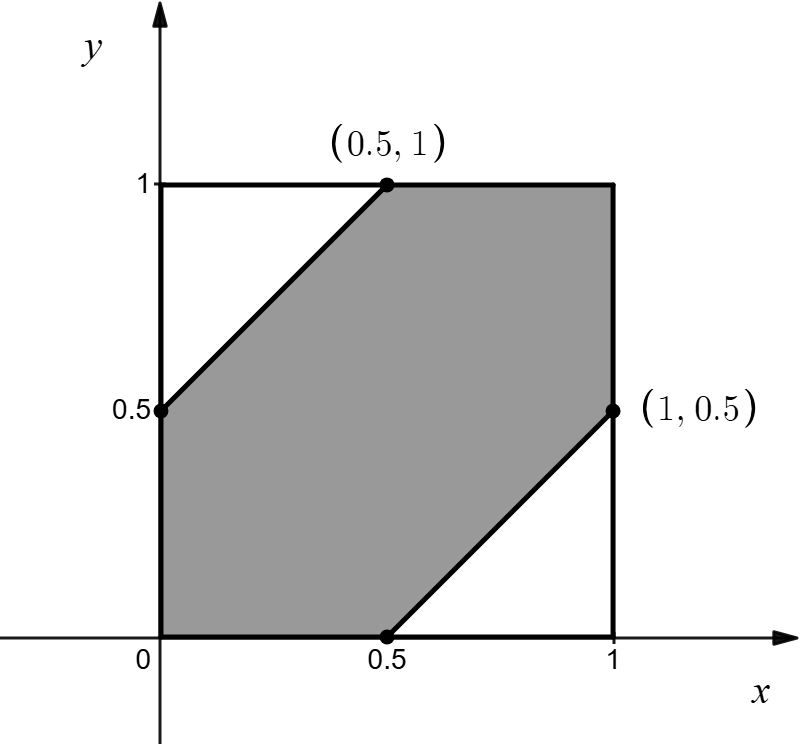
\includegraphics[width=\linewidth]{10.4.png}}  
\end{minipage}
\end{solution}
\begin{problem}
设$X$和$Y$是两个相互独立的随机变量,$X$在$(0,1)$上服从均匀分布,$Y$的概率密度为:
$$f_Y(y)=
\begin{cases}
	\dfrac{1}{2}\mathrm{e}^{-\tfrac{y}{2}}, &y>0\\
	0, &y\le0
\end{cases}$$
(1)求$X$和$Y$的联合概率密度;(2)设含有$a$的二次方程为$a^2+2Xa+Y=0$,试求$a$有实根的概率.
\end{problem}
\begin{solution}
(1)$X$的概率密度为$f_X(x)=
\begin{cases}
	1, &0<x<1\\
	0, &\text{其它}
\end{cases}$,因为$X$和$Y$相互独立,于是$f(x,y)=f_X(x)f_Y(y)=
\begin{cases}
	\dfrac{1}{2}\mathrm{e}^{-\tfrac{y}{2}}, &0<x<1,y>0\\
	0, &\text{其它}
\end{cases}$;\\
(2)$\Delta=(2X)^2-4Y\ge0\Rightarrow Y\le X^2$,于是$\displaystyle P=\int_{0}^{1}\int_{0}^{x^2}f(x,y)\d y\d x=0.1444$
\end{solution}

\begin{mdframed}[backgroundcolor=gray!40, hidealllines=true]
6$^*$.设随机变量$X$和$Y$相互独立,下表列出随机变量$(X,Y)$联合分布律及关于$X$和$Y$的边缘分布律中的部分数值,试将其余数值填入表中空白处.
$$
\begin{tabular}{|c|c|c|c|c|}
	\hline
	\diagbox{$X$}{$Y$} & $y_1$ & $y_2$ & $y_3$ & $P\left\{X=x_i\right\}=p_{i\cdot}$ \\
	\hline
	$x_1$ & 1/24 & 1/8 & 1/12 & 1/4\\
	\hline
	$x_2$ & 1/8 & 3/8 & 1/4 & 3/4\\
	\hline
	$P\left\{Y=y_j\right\}=p_{\cdot j}$ & 1/6 & 1/2 & 1/3 & 1 \\
	\hline
\end{tabular}
$$
\end{mdframed}

\newpaper
\section{随机变量函数的分布}
\noindent 一、填空题.\\ 
1.设随机变量$X$与$Y$相互独立,且均服从区间$(0,3)$上的均匀分布,则$P\left\{\max(X,Y)\le1\right\}=\uline{\dfrac{1}{9}}$
\\ 2.设$X$与$Y$为两个随机变量,且$P\left\{X\ge0,Y\ge0\right\}=\dfrac{3}{7}$,$P\left\{X\ge0\right\}=P\left\{Y\ge0\right\}=\dfrac{4}{7}$,则\\
$P\left\{\max(X,Y)\ge0\right\}=\uline{\dfrac{5}{7}}$\\
二、计算题.
\begin{problem}
设$X$与$Y$为两个独立的随机变量,其概率密度为分别为:
$$
f_X(x)=
\begin{cases}
	1, &0\le x\le1\\
	0, &\text{其它} 
\end{cases},
f_Y(y)=
\begin{cases}
	\mathrm{e}^{-y}, &y>0\\
	0, &\text{其它}
\end{cases}
$$
求随机变量$Z=X+Y$的概率密度.
\end{problem}
\begin{solution}
$\displaystyle f_Z(z)=\int_{-\infty}^{+\infty}f_X(x)f_Y(z-x)\d x$
,当结果不为0时,应有$0\le x\le1,z-x>0\Rightarrow0\le x\le \min(1,z)$.当$z\ge1$时,$\displaystyle f_Z(z)=\int_{0}^{1}f_X(x)f_Y(z-x)\d x=\mathrm{e}^{-z}(\mathrm{e}-1)$;当$0<z<1$时,$\displaystyle f_Z(z)=\int_{0}^{z}f_X(x)f_Y(z-x)\d x=1-\mathrm{e}^{-z}$.于是$f_Z(z)=
\begin{cases}
	0,&z\le0\\
	1-\mathrm{e}^{-z},&0<z<1\\
	\mathrm{e}^{-z}(\mathrm{e}-1),&z\ge 1
\end{cases}$
\end{solution}
\begin{problem}
设$X$与$Y$为两个独立的随机变量,其概率密度分别为:
$$
f_X(x)=
\begin{cases}
	\lambda\mathrm{e}^{-\lambda x}, &x>0\\
	0,&x\le0
\end{cases},
f_Y(y)=
\begin{cases}
	\mu\mathrm{e}^{-\mu y}, &y>0\\
	0, &y\le0
\end{cases},
(\lambda,\mu>0\text{为常数})
$$
引入随机变量$Z=
\begin{cases}
	1,&X\le Y\\
	0,&X>Y
\end{cases}$,
(1)求条件概率密度$f_{X\mid Y}(x\mid y)$;
(2)求$Z$的分布律与分布函数.
\end{problem}
\begin{solution}
(1)因为$X$与$Y$相互独立,故$f_{X\mid Y}(x\mid y)=f_X(x)=
\begin{cases}
	\lambda\mathrm{e}^{-\lambda x}, &x>0\\
	0,&x\le0
\end{cases}$;\\
(2)$\displaystyle P\left\{Z=1\right\}=P\left\{X\le Y\right\}=\int_{0}^{+\infty}\int_{0}^{y}f_X(x)f_Y(y)\d x\d y=\int_{0}^{+\infty}\int_{0}^{y}\lambda\mu\mathrm{e}^{-(\lambda x+\mu y)}\d x\d y=\dfrac{\lambda}{\lambda+\mu}$,$P\left\{Z=0\right\}=1-P\left\{Z=1\right\}=\dfrac{\mu}{\mu+\lambda}$.分布函数$F_Z(z)=
\begin{cases}
	0,&z<0\\
	\dfrac{\mu}{\mu+\lambda},&0\le z<1\\
	1,&z\ge1
\end{cases}$
\end{solution}
\newpaper
\begin{problem}
设某种型号的电子元件的寿命(于小时计)近似地服从$N(160,20^2)$分布,随机地取4只,求其中没有一只寿命小于180的概率.
\end{problem}
\begin{solution}
即4只寿命均大于180的概率,记$X_i$为第$i$个电子元件的寿命,$P\left\{X_i>\mu+\sigma\right\}=1-P\left\{X_i\le\mu+\sigma\right\}=1-\varPhi(1)=0.1587$,$\displaystyle \prod_{i=1}^{4} P\left\{X_i>\mu+\sigma\right\}=6.343\times10^{-4}$
\end{solution}
\begin{problem}
设$X$与$Y$相互独立,$P\left\{X=i\right\}=\dfrac{1}{3},(i=-1,0,1)$,$Y$的概率密度为$f_Y(y)=
\begin{cases}
	1,&0\le y\le1\\
	0,&\text{其它}
\end{cases}$,记$Z=X+Y$,
(1)求$P\left\{Z\le\dfrac{1}{2}\middle| X=0\right\}$;
(2)用全概率公式计算$P\left\{Z\le1.4\right\}$.
\end{problem}
\begin{solution}
(1)$\displaystyle P\left\{Z\le\dfrac{1}{2}\middle| X=0\right\}=P\left\{Y\le\dfrac{1}{2}\right\}=\int_{0}^{\tfrac{1}{2}}f_Y(y)\d y=\dfrac{1}{2}$;\\
(2)$P\left\{Z\le1.4\right\}=P\left\{X=-1\right\}P\left\{Y\le2.4\right\}+P\left\{X=0\right\}P\left\{Y\le1.4\right\}+P\left\{X=1\right\}P\left\{Y\le0.4\right\}=\dfrac{1}{3}\times(1+1+0.4)=0.8$
\end{solution}
\begin{problem}
设随机变量$X,Y$相互独立,且服从同一分布.试证明:
$$
P\left\{a<\min(X,Y)\le b\right\}=\left[P\left\{X>a\right\}\right]^2-\left[P\left\{X>b\right\}\right]^2
$$
\end{problem}
\begin{solution}
$P\left\{a<\min(X,Y)\le b\right\}=P\left\{\min(X,Y)> a\right\}-P\left\{\min(X,Y)>b\right\}=P\left\{X>a,Y>a\right\}-\\
P\left\{X>b,Y>b\right\}=P\left\{X>a\right\}P\left\{Y>a\right\}-P\left\{X>b\right\}P\left\{Y>b\right\}=\left[P\left\{X>a\right\}\right]^2-\left[P\left\{X>b\right\}\right]^2$
\end{solution}
\newpaper
\section{数学期望}
\noindent 一、填空题.\\ 
1.$X$服从参数为1的指数分布,则$E(2X+3\mathrm{e}^{-2X})=\uline{3}$\\
2.$X\sim \pi(1)$,则$P\left\{X=2E(X)\right\}=\uline{\dfrac{1}{2\mathrm{e}}}$\\
二、计算题.
\begin{problem}
某产品的次品率为0.1,检验员每天检验4次,每次随机地取10件产品进行检验,如发现其中的次品数多于1,就去调整设备,以$X$表示一天中调整设备的次数,试求$E(X)$.(设各产品是否为次品是相互独立的)
\end{problem}
\begin{solution}
记$X_i$:第$i(i=1,2,3,4)$次检验的调整次数,$P\left\{X_i=0\right\}=0.9^{10}+C^1_{10}(0.1)(0.9)^9\approx0.74$,$P\left\{X_i=1\right\}\\
=1-P\left\{X_i=0\right\}=0.26$,故$E(X_i)=0.26$,于是$\displaystyle E(X)=\sum_{i=1}^{4}E(X_i)=4\times0.26=1.04$
\end{solution}
\begin{problem}
设随机变量$X$与$Y$的联合概率分布如下:
$$
\begin{tabular}{|c|c|c|c|}
	\hline
	\diagbox{$X$}{$Y$} & $-1$ & $0$ & $1$   \\
	\hline
	$0$ & 0.07 & 0.18 & 0.15 \\
	\hline
	$1$ & 0.08 & 0.32 & 0.20 \\
	\hline
\end{tabular}
$$
求$E(X)$,$E(Y)$,$E(XY)$.
\end{problem}
\begin{solution}
$E(X)=1\times0.6=0.6$,$E(Y)=-1\times0.15+1\times0.35=0.2$,\\
$E(XY)=1\times(-1)\times0.08+1\times1\times0.2=0.12$
\end{solution}
\begin{problem}
设$(X,Y)$的概率密度为$f(x,y)=
\begin{cases}
	12y^2, &0\le y\le x\le 1\\
	0,&\text{其它}
\end{cases}$\\
求$E(X)$,$E(Y)$,$E(XY)$,$E(X^2+Y^2)$.
\end{problem}
\begin{solution}
$\displaystyle E(X)=\int_{0}^{1}\int_{y}^{1}xf(x,y)\d x\d y=\dfrac{4}{5}$,$\displaystyle E(Y)=\int_{0}^{1}\int_{0}^{x}yf(x,y)\d y\d x=0.6$,\\
$\displaystyle E(XY)=\int_{0}^{1}\int_{y}^{1}xyf(x,y)\d x\d y=\dfrac{1}{2}$,$\displaystyle E(X^2+Y^2)=\int_{0}^{1}\int_{y}^{1}(x^2+y^2)f(x,y)\d x\d y=\dfrac{16}{15}$
\end{solution}
\begin{problem}
将$n$只球($1\sim n$号)随机地放进$n$只盒子($1\sim n$号)中去,一只盒子装一只球.若一只球装入与球同号的盒子中,称为一个配对,记$X$为总的配对数,求$E(X)$.
\end{problem}
\begin{solution}
$i$号盒子的配对情况记为$X_i=
\begin{cases}
	0,&\text{不配对} \\
	1,&\text{配对}
\end{cases}$,
$P\left\{X_i=1\right\}=\dfrac{(n-1)!}{n!}=\dfrac{1}{n}$,故$E(X_i)=\dfrac{1}{n}$,于是\\
$\displaystyle E(X)=\sum_{i=1}^{n}E(X_i)=1$
\end{solution}
\newpaper
\section{方差}
\noindent 一、填空题.\\ 
1.设$X\sim b(n,p)$,则$E(X)=\uline{np}$,$D(X)=\uline{np(1-p)}$\\
2.设$X\sim \pi(\lambda)$,则$E(X)=\uline{\lambda}$,$D(X)=\uline{\lambda}$\\
3.设$X\sim U(a,b)$,则$E(X)=\uline{\dfrac{a+b}{2}}$,$D(X)=\uline{\dfrac{(b-a)^2}{12}}$\\ 
4.设$X$服从参数为$\theta$的指数分布,则$E(X)=\uline{\theta}$,$D(X)=\uline{\theta^2}$\\ 
5.设$X\sim N(\mu,\sigma^2)$,则$E(X)=\uline{\mu}$,$D(X)=\uline{\sigma^2}$\\
6.已知随机变量$X\sim N(-3,1)$,$Y\sim N(2,1)$,且$XY$相互独立,$Z=X-2Y+7$,则$Z\sim \uline{N(0,5)}$\\              
二、计算题.
\begin{problem}
设随机变量$X_1,X_2,X_3,X_4$相互独立,且有$E(X_i)=i$,$D(X_i)=5-i$,$(i=1,2,3,4)$.设$Y=2X_1-X_2+3X_3-\dfrac{1}{2}X_4$,求$E(Y)$,$D(Y)$.
\end{problem}
\begin{solution}
$E(Y)=2E(X_1)-E(X_2)+3E(X_3)-\dfrac{1}{2}E(X_4)=7$,\\
$D(Y)=2^2D(X_1)+D(X_2)+3^2D(X_3)+\dfrac{1}{4}D(X_4)=37.25$	
\end{solution}
\begin{problem}
卡车装运水泥,设每袋水泥的重量$X$(以公斤记)服从$N(50,2.5^2)$,问最多装多少袋水泥使总重量超过2000的概率不大于0.05.
\end{problem}
\begin{solution}
记$\displaystyle Y=\sum_{i=1}^{n}X_i$,则$E(Y)=nE(X)$,$D(Y)=nD(X)$,那么$P\left\{\dfrac{Y-E(Y)}{\sqrt{D(Y)}}>\dfrac{2000-50n}{2.5\sqrt{n}}\right\}=1-\\\varPhi\left(\dfrac{2000-50n}{2.5\sqrt{n}}\right)\le 0.05$,查表得$\dfrac{2000-50n}{2.5\sqrt{n}}\ge1.65$,解得$n\le 39$
\end{solution}
\begin{problem}
设随机变量$X,Y$相互独立,且$X\sim N(6,16)$,$Y\sim N(1,9)$,求\\(1)$P\left\{X>Y\right\}$;(2)$P\left\{X+Y\ge 7\right\}$.
\end{problem}
\begin{solution}
(1)因为$X-Y\sim N(5,25)$,所以$P\left\{X>Y\right\}=P\left\{X-Y>0\right\}=P\left\{\dfrac{X-Y-5}{5}>\dfrac{0-5}{5}\right\}=1-\varPhi(-1)=\varPhi(1)=0.8413$;\\
(2)因为$X+Y\sim N(7,25)$,所以$P\left\{X+Y\ge7\right\}=P\left\{\dfrac{X+Y-7}{5}\ge\dfrac{7-7}{5}\right\}=1-\varPhi(0)=0.5000$
\end{solution}
\begin{problem}
设$X$为随机变量,$C$为常数,证明$D(X)\le E\left\{(X-C)^2\right\}$.
\end{problem}
\begin{solution}
$E\left\{(X-C)^2\right\}=E(X^2+C^2-2CX)=E(X^2)-2CE(X)+C^2=E(X^2)-\left[E(X)\right]^2+\left[E(X)-C\right]^2\ge D(X)$
\end{solution}
\newpaper
\section{协方差与相关系数}
\noindent 一、填空题\\ 1.设$E(X)=-1$,$D(X)=1$,$E(Y)=1$,$D(Y)=2$,$\mathrm{Cov}(X,Y)=1$,则$E(3X+4Y)=\uline{1}$,$D(3X-4Y)=\uline{17}$\\
2.设$D(X)=2$,$D(Y)=3$,$\mathrm{Cov}(X,Y)=-1$,则
$\mathrm{Cov}(3X-2Y+1, X+4Y-3)=\uline{-28}$\\
3.设$X\sim N(0,1)$,$Y\sim N(1,4)$,$\rho_{_{XY}} = 1$,则$P\left\{Y=2X+1\right\}=\uline{1}$\\
4.设$(X,Y)\sim N(\mu_1,\mu_2,\sigma^2_1,\sigma^2_2,\rho)$,则$X$和$Y$相互独立的充要条件是$\rho=\uline{0}$\\
二、计算题.
\begin{problem}
设随机变量$(X,Y)$具有概率密度:
$$
f(x,y)=
\begin{cases}
	\dfrac{1}{8}(x+y), &0\le x\le 2,0\le y\le 2\\
	0, &\text{其它}
\end{cases}
$$
求$E(X)$,$E(Y)$,$\mathrm{Cov}(X,Y)$,$\rho_{_{XY}}$,$D(X+Y)$.
\end{problem}
\begin{solution}
$\displaystyle E(X)=\int_{0}^{2}\int_{0}^{2}xf(x,y)\d x\d y=\dfrac{7}{6}$,
$\displaystyle 
D(X)=\int_{0}^{2}\int_{0}^{2}x^2f(x,y)\d x\d y-[E(X)]^2=\dfrac{11}{36}$,\\
$\displaystyle E(Y)=\int_{0}^{2}\int_{0}^{2}yf(x,y)\d x\d y=\dfrac{7}{6}$,
$\displaystyle D(Y)=\int_{0}^{2}\int_{0}^{2}y^2f(x,y)\d x\d y-[E(Y)]^2=\dfrac{11}{36}$,\\
$\displaystyle E(XY)=\int_{0}^{2}\int_{0}^{2}xyf(x,y)\d x\d y=\dfrac{4}{3}$,
$\mathrm{Cov}(X,Y)=E(XY)-E(X)E(Y)=-\dfrac{1}{36}$,\\
$\rho_{_{XY}}=\dfrac{\mathrm{Cov}(X,Y)}{\sqrt{D(X)}\sqrt{D(Y)}}=-\dfrac{1}{11}$,
$\displaystyle D(X+Y)=D(X)+D(Y)+2\mathrm{Cov}(X,Y)=\dfrac{5}{9}$
\end{solution}
\begin{problem}
设二维随机变量$(X,Y)$的概率密度为:$f(x,y)=
\begin{cases}
	\dfrac{1}{\pi}, &x^2+y^2=1\\
	0, &\text{其它}
\end{cases}$,试验证$X$和$Y$是不相关的,但$X$和$Y$不是相互独立的.
\end{problem}
\begin{solution}
$\displaystyle E(X)=\int_{-1}^{1}\int_{-\sqrt{1-y^2}}^{\sqrt{1-y^2}}xf(x,y)\d x\d y=0$,
$\displaystyle E(Y)=\int_{-1}^{1}\int_{-\sqrt{1-x^2}}^{\sqrt{1-x^2}}yf(x,y)\d y\d x=0$,\\
$\displaystyle E(XY)=\int_{-1}^{1}\int_{-\sqrt{1-y^2}}^{\sqrt{1-y^2}}xyf(x,y)\d x\d y=0$,
$\mathrm{Cov} (X,Y)=E(XY)-E(X)E(Y)=0$,\\
当$x^2+y^2=1$时,
$\displaystyle f_X(x)=\int_{-\sqrt{1-x^2}}^{\sqrt{1-x^2}}f(x,y)\d y=\dfrac{2}{\pi}\sqrt{1-x^2}$,
$\displaystyle f_Y(y)=\int_{-\sqrt{1-y^2}}^{\sqrt{1-y^2}}f(x,y)\d x=\dfrac{2}{\pi}\sqrt{1-y^2}$,\\
$f_X(x)f_Y(y)\ne f(x,y)$,故$X$和$Y$是不相关的,但不是相互独立的
\end{solution}
\begin{problem}
设$(X,Y)$服从二维正态分布,且有$D(X)=\sigma_X^2$,$D(Y)=\sigma_Y^2$,证明当$a^2=\sigma_X^2/\sigma_Y^2$时随机变量$W=X-aY$与$V=X+aY$相互独立.
\end{problem}
\begin{solution}
二维正态分布分量线性组合仍是正态分布,其独立与不相关等价,$E(WV)=E(X^2-a^2Y^2)=E(X^2)-a^2E(Y^2)=\sigma^2_X+\mu_X^2-a^2(\sigma_Y^2+\mu_Y^2)$,$E(W)E(V)=\mu_X^2-a^2\mu_Y^2$,$\mathrm{Cov}(W,V)=E(WV)-E(W)E(V)=\sigma_X^2-a^2\sigma_Y^2=0$,故当$a^2=\sigma_X^2/\sigma_Y^2$时随机变量$W=X-aY$与$V=X+aY$相互独立
\end{solution}
\newpaper
\section{大数定律与中心极限定理}
\noindent 一、填空题.\\
1.设随机变量$X$具有$E(X)=\mu$,$D(X)=\sigma^2$,则由切比雪夫不等式,有$P\left\{\left|X-\mu\right|\ge3\sigma\right\}\le\uline{\dfrac{1}{9}}$\\
2.设$X_1,X_2,\cdots,X_n,\cdots$相互独立同分布,且$E(X_n)=0$,则$\displaystyle\lim_{n \to \infty}P\left\{\left|\sum_{i=1}^{n}X_i\right|<n\right\}=\uline{1}$\\
二、计算题.
\begin{problem}
计算器在进行加法时,将每个加数舍入最靠近它的整数.设所有舍入误差是独立的且在$(-0.5,0.5)$上服从均匀分布,(1)若将1500个数相加,问误差总和的绝对值超过15的概率是多少?(2)最多可有几个数相加使得误差总和的绝对值小于10的概率不小于0.90?
\end{problem}
\begin{solution}
每个数的舍入误差记为$X_i$,$\displaystyle Y=\sum_{i=1}^{n}X_i$,由题意得$X_i\sim U(-0.5,0.5)$,$E(X_i)=0$,$D(X_i)=\dfrac{1}{12}$,$E(Y)=0$,$D(Y)=\dfrac{n}{12}$.当$k\ge0$时,$P\left\{\left|Y\right|<k\right\}=P\left\{\left|\dfrac{Y}{\sqrt{n/12}}\right|<\dfrac{k}{\sqrt{n/12}}\right\}=2\varPhi\left(2k\sqrt{\dfrac{3}{n}}\right)-1$,则\\
(1)$n=1500$,$k=15$,$P\left\{\left|Y\right|>15\right\}=2-2\varPhi\left(\dfrac{3}{5}\sqrt{5}\right)\approx2-2\varPhi(1.34)=0.1802$;\\
(2)$k=10$,$2\varPhi\left(20\sqrt{\dfrac{3}{n}}\right)-1\ge0.90$,查表得$20\sqrt{\dfrac{3}{n}}\ge1.65$,解得$n\le440$
\end{solution}
\begin{problem}
设有1000个人独立行动,每个人能够按时进入隐蔽体的概率为0.9,以95\%概率估计,在一次行动中,至少有多少人能够进入?
\end{problem}
\begin{solution}
设进入的人数为$X$,$X\sim b(1000,0.9)$,$P\left\{X\ge k\right\}=1-\varPhi\left(\dfrac{k-900}{3\sqrt{10}}\right)=0.95$,查表得$\dfrac{900-k}{3\sqrt{10}}=1.65$,解得$k=884$
\end{solution}
\begin{problem}
在一家保险公司里有10000人参加保险,每人每年付12元保险费,在一年内一个人死亡的概率为0.006,死亡者其家属可向保险公司领得1000元赔偿费,求:\\
(1)保险公司没有利润的可能性有多大?(2)保险公司一年的利润不少于60000元的概率为多大?
\end{problem}
\begin{solution}
设一年内死亡的人数为$X$,由题意知$X\sim b(10000,0.006)$,$E(X)=60$,$D(X)=59.64$\\
(1)由题意知$1000X>120000\Rightarrow X>120$,$P\left\{X>120\right\}=P\left\{\dfrac{X-60}{\sqrt{59.64}}>\dfrac{120-60}{\sqrt{59.64}}\right\}\approx1-\varPhi(7.77)\approx0$\\
(2)由题意知$1000X\le60000\Rightarrow X\le60$,$P\left\{X\le60\right\}=P\left\{\dfrac{X-60}{\sqrt{59.64}}\le\dfrac{60-60}{\sqrt{59.64}}\right\}=\varPhi(0)=0.5$
\end{solution}
\begin{problem}
一复杂的系统由$n$个相互独立起作用的部件所组成,每个部件的可靠性为0.90,且必须至少有80\%的部件工作才能使整个系统正常工作,问$n$至少为多大才能使系统的可靠性不低于0.95?
\end{problem}
\begin{solution}
设正常工作的零件数为$X$,$X\sim b(n,0.9)$,$E(X)=0.9n$,$D(X)=0.09n$,由题意知$P\left\{X\ge0.8n\right\}=1-\varPhi\left(\dfrac{0.8n-0.9n}{\sqrt{0.09n}}\right)=\varPhi\left(\dfrac{\sqrt{n}}{3}\right)\ge0.95$,查表得$\dfrac{\sqrt{n}}{3}\ge1.65$,得$n\ge25$
\end{solution}
\newpaper
\section{样本及抽样分布(一)}
\noindent 一、填空题.\\
1.设$X_1,X_2,\cdots,X_n$为来自总体$N(0,\sigma^2)$的
样本,且随机变量$\displaystyle Y=C(\sum_{i=1}^{n}X_i)^2\sim \chi^2(1)$,则常数$C=\uline{\dfrac{1}{n\sigma^2}}$\\
2.设$(X_1,X_2,X_3,X_4)$取自正态总体$X\sim N(0,2^2)$的样本,且$Y=\dfrac{1}{20}(X_1-2X_2)^2+\dfrac{1}{100}(3X_3-4X_4)^2$,则$Y\sim\uline{\chi^2(2)}$分布.\\
二、计算题.
\begin{problem}
在总体$N(52,3^2)$中随机抽一容量为36的样本,求样本均值$\overline{X}$落在50.8到53.8之间的概率.
\end{problem}
\begin{solution}
$E(\overline{X})=\mu=52$,$D(\overline{X})=\dfrac{\sigma^2}{n}=\dfrac{1}{4}$,$P\left\{50.8\le\overline{X}\le53.8\right\}=P\left\{\overline{X}<53.8\right\}-P\left\{\overline{X}<50.8\right\}=\varPhi\left(\dfrac{53.8-52}{\sqrt{0.25}}\right)-\varPhi\left(\dfrac{50.8-52}{\sqrt{0.25}}\right)=\varPhi(3.6)+\varPhi(2.4)-1=0.9916$
\end{solution}
\begin{problem}
求总体$N(20,3)$的容量分别为$10,15$的两独立样本均值差的绝对值大于0.3的概率.
\end{problem}
\begin{solution}
设样本均值分别为$\overline{X},\overline{Y}$,则$\overline{X}\sim N(20,0.3)$,$\overline{Y}\sim N(20,0.2)$,$\overline{X}-\overline{Y}\sim N(0,0.5)$,于是\\
$P\left\{\left|\overline{X}-\overline{Y}\right|>0.3\right\}=P\left\{\overline{X}-\overline{Y}>0.3\right\}+P\left\{\overline{X}-\overline{Y}<-0.3\right\}=2-2\varPhi\left(\dfrac{0.3}{\sqrt{0.5}}\right)=0.6744$
\end{solution}
\begin{problem}
设$X_1,X_2,\cdots,X_{10}$为$N(0,0.3^2)$的一个样本,求$\displaystyle P\left\{\sum_{i=1}^{10}X^2_i>1.44\right\}$.
\end{problem}
\begin{solution}
由题意知$\dfrac{X_i}{0.3}\sim N(0,1)$,则$\displaystyle\dfrac{100}{9}\sum_{i=1}^{10}X_i^2\sim\chi^2(10)$,$\displaystyle P\left\{\sum_{i=1}^{10}X_i^2>1.44\right\}=P\left\{\chi^2(10)>16\right\}\approx0.1$
\end{solution}
\begin{problem}
设总体$X\sim \chi^2(n)$,$X_1,X_2,\cdots,X_{10}$是来自$X$的样本,求$E(\overline{X})$,$D(\overline{X})$,$E(S^2)$.
\end{problem}
\begin{solution}
$E(\overline{X})=E(X)=n$,$D(\overline{X})=\dfrac{D(X)}{10}=\dfrac{n}{5}$,$E(S^2)=D(X)=2n$
\end{solution}
\newpaper
\section{样本及抽样分布(二)}
\noindent 一、填空题.\\
1.设总体$X\sim N(\mu,\sigma^2)$,$X_1,X_2,\cdots,X_n$为来自$X$的样本,则$\displaystyle\dfrac{(n-1)S^2}{\sigma^2}=\sum_{i=1}^{n}\dfrac{(X_i-\overline{X})^2}{\sigma^2}\sim\uline{\chi^2(n-1)}$分布,$\displaystyle\sum_{i=1}^{n}\dfrac{(X_i-\mu)^2}{\sigma^2}\sim\uline{\chi^2(n)}$分布.\\
2.记$t_\alpha(n)$为$t$分布的上$\alpha$分位点,则$t_{0.995}(29)=\uline{-2.7564}$\\
3.已知$X\sim t(n)$,则$X^2\sim\uline{F(1,n)}$分布\\
二、解答题.
\begin{problem}
设总体$X\sim B(1,p)$,设$X_1,X_2,\cdots,X_n$是来自$X$的样本.\\
(1)求$(X_1,X_2,\cdots,X_n)$的分布律;(2)求$\displaystyle\sum_{i=1}^{n}X_i$的分布律;(3)求$E(\overline{X})$,$D(\overline{X})$,$E(S^2)$.
\end{problem}
\begin{solution}
(1)$P\left\{X_1=x_1,X_2=x_2,\cdots,X_n=x_n\right\}=p^{\sum_{i=1}^{n}x_i}(1-p)^{n-\sum_{i=1}^{n}x_i},x_i=0,1$;\\
(2)$P\displaystyle\left\{\sum_{i=1}^{n}X_i=k\right\}=C_n^kp^k(1-p)^{n-k},k=1,2,\cdots,n$;\\
(3)$E(\overline{X})=E(X)=p$,$D(\overline{X})=\dfrac{D(X)}{n}=\dfrac{p(1-p)}{n}$,$E(S^2)=D(X)=p(1-p)$
\end{solution}
\begin{problem}
设在总体$N(\mu,\sigma^2)$中抽取一容量为16的样本,这里$\mu,\sigma^2$均为未知.\\
(1)求$P\left\{\dfrac{S^2}{\sigma^2}\le2.041\right\}$,其中$S^2$为样本方差;(2)求$D(S^2)$
\end{problem}
\begin{solution}
(1)$P\left\{\dfrac{15S^2}{\sigma^2}\le2.041\times15\right\}=P\left\{\chi^2(15)\le30.615\right\}=1-P\left\{\chi^2(15)>30.615\right\}=0.99$;\\
(2)$D\left(\dfrac{15S^2}{\sigma^2}\right)=2\times15\Rightarrow D(S^2)=\dfrac{2\sigma^4}{15}$
\end{solution}
\begin{problem}
设总体$X\sim N(\mu,\sigma^2)$,$X_1,X_2,X_3,X_4$为来自$X$的样本,$Y=\dfrac{X_3-X_4}{\sqrt{\sum_{i=1}^{2}(X_i-\mu)^2}}$,证明$Y\sim t(2)$.
\end{problem}
\begin{solution}
$Y=\dfrac{\dfrac{X_3-X_4}{\sqrt{2}\sigma}}{\sqrt{\dfrac{1}{2} \displaystyle\sum_{i=1}^{2} \left( \dfrac{X_i-\mu}{\sigma} \right)^2}}$,$\dfrac{X_3-X_4}{\sqrt{2}\sigma}\sim N(0,1)$,$\displaystyle\sum_{i=1}^{2}\left(\dfrac{X_i-\mu}{\sigma}\right)^2\sim\chi(2)$,故$Y\sim t(2)$
\end{solution}
\newpaper
\section{点估计}
\begin{problem}
设$X_1,X_2,\cdots,X_n$为总体$X$的一个样本,$X$的密度函数为:\\$f(x)=
\begin{cases}
\sqrt{\theta}x^{\sqrt{\theta}-1},&0\le x\le 1\\
0,&\text{其它}
\end{cases},(\theta>0)$,求$\theta$的矩估计和最大似然估计.
\end{problem}
\begin{solution}
$\displaystyle E(X)=\int_{0}^{1}xf(x)\d x=\dfrac{\sqrt{\theta}}{\sqrt{\theta}+1}=\mu_1$,则$\sqrt{\theta}=\dfrac{\mu_1}{1-\mu_1}\Rightarrow\hat{\theta}=\left(\dfrac{\overline{X}}{1-\overline{X}}\right)^2$\\
$\displaystyle L(\theta)=\prod_{i=1}^{n}f(x_i)=\theta^{\tfrac{n}{2}}\left(\prod_{i=1}^{n}x_i\right)^{\sqrt{\theta}-1}$,$\displaystyle\ln L(\theta)=\dfrac{n}{2}\ln\theta+(\sqrt{\theta}-1)\sum_{i=1}^{n}\ln x_i$,$\dfrac{\d\ln L(\theta)}{\d\theta}=\dfrac{n}{2\theta}+\dfrac{\sum_{i=1}^{n}\ln x_i}{2\sqrt{\theta}}=0$,解得$\hat{\theta}=\dfrac{n^2}{(\sum_{i=1}^{n}\ln x_i)^2}$,故$\hat{\theta}=\dfrac{n^2}{(\sum_{i=1}^{n}\ln X_i)^2}$
\end{solution}
\begin{problem}
设某种元件的使用寿命$X$的概率密度为$f(x;\theta)=
\begin{cases}
2\mathrm{e}^{-2(x-\theta)},&x>\theta\\
0,&\text{其它}
\end{cases}$,其中$\theta>0$为未知参数,又设$x_1,x_2,\cdots,x_n$是$X$的一组样本观测值,求参数$\theta$的最大似然估计值.
\end{problem}
\begin{solution}
$L(\theta)=2^n\mathrm{e}^{2n\theta}\cdot\mathrm{e}^{-2\sum_{i=1}^{n}x_i}$,$\displaystyle\ln L(\theta)=n\ln2+2n\theta-2\sum_{i=1}^{n}x_i$,$\dfrac{\d\ln L(\theta)}{\d\theta}=2n>0$,又$f(x;\theta)\ge0$,于是$\theta\le x_i$,则$\hat{\theta}=\text{min}(x_1,x_2,\cdots,x_n)$
\end{solution}
\begin{problem}
设$X_1,X_2,\cdots,X_n$是来自总体$X$的一个样本,且$X\sim \pi(\lambda)$,求$P\left\{X=0\right\}$的最大似然估计.
\end{problem}
\begin{solution}
$L(\lambda)=\mathrm{e}^{-n\lambda}\dfrac{\lambda^{\sum_{i=1}^{n}x_i}}{\prod_{i=1}^{n}x_i!}$,$\displaystyle\ln L(\lambda)=-n\lambda+\ln\lambda\sum_{i=1}^{n}x_i-\sum_{i=1}^{n}\ln x_i!$,$\dfrac{\d\ln L(\lambda)}{\d\lambda}=-n+\dfrac{\sum_{i=1}^{n}x_i}{\lambda}=0$,解得$\displaystyle \hat{\lambda}=\dfrac{1}{n}\sum_{i=1}^{n}x_i=\overline{x}$,故$\displaystyle \hat{\lambda}=\dfrac{1}{n}\sum_{i=1}^{n}X_i=\overline{X}$,$P\left\{X=0\right\}$的最大似然估计为$\mathrm{e}^{-\overline{X}}$
\end{solution}
\begin{problem}
设总体$X$具有分布律(如下表),其中$\theta(0<\theta<1)$为未知参数.已知取得了样本值$x_1=1,x_2=2,x_3=1$.试求$\theta$的矩估计值和最大似然估计值.
$$
\begin{tabular}{|c|c|c|c|}
	\hline
	$X$ & 1 & 2 & 3  \\
	\hline
	$p$ & $\theta^2$ & $2\theta(1-\theta)$ & $(1-\theta)^2$  \\
	\hline
\end{tabular}
$$
\end{problem}
\begin{solution}
$\mu_1=E(X)=-2\theta+3\Rightarrow\hat{\theta}=\dfrac{3-\overline{x}}{2}=\dfrac{5}{6}$,$L(\theta)=\theta^2\cdot2\theta(1-\theta)\cdot\theta^2=2\theta^5(1-\theta)$,$\ln L(\theta)=\ln 2 +5\ln\theta+\ln(1-\theta)$,$\dfrac{\d\ln L(\theta)}{\d\theta}=\dfrac{5}{\theta}-\dfrac{1}{1-\theta}=\dfrac{5-6\theta}{\theta(1-\theta)}=0\Rightarrow\hat{\theta}=\dfrac{5}{6}$
\end{solution}
\newpaper
\section{估计量的评价标准}
\noindent 一、填空题.\\
1.设$X_1,X_2,\cdots,X_n$是来自总体$B(n,p)$的样本,若$\overline{X}+kS^2$为$np^2$的无偏估计,则$k=\uline{-1}$\\
2.设$X_1,X_2,\cdots,X_n$是来自总体$N(\mu,\sigma^2)$的样本,若$\displaystyle a\sum_{i=1}^{n}(X_i-\mu)^2$和$\displaystyle b\sum_{i=1}^{n}(X_i-\overline{X})^2$都是$\sigma^2$的无偏估计,则$a=\uline{\dfrac{1}{n}}$,$b=\uline{\dfrac{1}{n-1}}$\\
二、解答题.
\begin{problem}
设$X_1,X_2,\cdots,X_n$是来自总体$X$的一个样本,设$E(X)=\mu$,$D(X)=\sigma^2$.\\
(1)确定常数$c$使$\displaystyle c\sum_{i=1}^{n-1}(X_{i+1}-X_i)^2$为$\sigma^2$的无偏估计;(2)确定常数$c$使$(\overline{X})^2-cS^2$为$\mu^2$的无偏估计.
\end{problem}
\begin{solution}
(1)$\displaystyle E\left[ c\sum_{i=1}^{n-1}(X_{i+1}-X_i)^2\right]=cE\left(\sum_{i=1}^{n-1}X_{i+1}^2-2X_{i+1}X_{i}+X_i^2\right)=c\sum_{i=1}^{n-1}E(X_{i+1}^2-2X_{i+1}X_{i}+X_i^2)=c\sum_{i=1}^{n-1}E(X_{i+1}^2)+E(X_i^2)-2E(X_{i+1})E(X_{i})=2c(n-1)\sigma^2=\sigma^2$,于是$c=\dfrac{1}{2(n-1)}$;\\
(2)$\displaystyle E\left[(\overline{X})^2-cS^2\right]=E\left[(\overline{X})^2\right]-cE(S^2)=\mu^2+\dfrac{\sigma^2}{n}-c\sigma^2=\mu^2$,于是$c=\dfrac{1}{n}$
\end{solution}
\begin{problem}
设$X_1,X_2,X_3,X_4$是来自均值$\theta$的指数分布总体的样本.其中$\theta$未知.设有估计量:
$$
T_1=\dfrac{1}{6}(X_1+X_2)+\dfrac{1}{3}(X_3+X_4)\quad
T_2=\dfrac{1}{5}(X_1+2X_2+3X_3+4X_4)\quad
T_3=\dfrac{1}{4}(X_1+X_2+X_3+X_4)
$$
(1)指出其中哪几个是$\theta$的无偏估计量;(2)在上述$\theta$的无偏估计量中指出哪一个较为有效.
\end{problem}
\begin{solution}
(1)$E(X_i)=\theta,1\le i \le 4$,$E(T_1)=\theta$,$E(T_2)=2\theta$,$E(T_3)=\theta$,故$T_1,T_3$是$\theta$的无偏估计量;\\
(2))$D(X_i)=\theta^2,1\le i \le 4$,$D(T_1)=\dfrac{5}{18}\theta^2$,$D(T_3)=\dfrac{1}{4}\theta^2$,$D(T_1)>D(T_3)$,故$T_3$更为有效
\end{solution}
\begin{problem}
设$\hat{\theta}$是参数$\theta$的无偏估计量,并有$D(\hat{\theta})>0$,试证$\hat{\theta}^2=(\hat{\theta})^2$不是$\theta^2$的无偏估计.
\end{problem}
\begin{solution}
$E(\hat{\theta})=\theta$,$D(\hat{\theta})=E(\hat{\theta}^2)-\theta^2>0$,证毕
\end{solution}
\newpaper
\section{正态总体均值与方差的区间估计}
\begin{problem}
设总体$X\sim N(\mu,8)$,$(X_1,X_2,\cdots,X_{36})$为其简单随机样本,$\left[\overline{X}-1,\overline{X}+1\right]$是$\mu$的一个置信区间,求该置信区间的置信水平.
\end{problem}
\begin{solution}
$\dfrac{\sigma}{\sqrt{n}}z_{\alpha/2}=1\Rightarrow z_{\alpha/2}=2.12$,查表得$\alpha=0.034$,置信水平为$1-\alpha=0.966$
\end{solution}
\begin{problem}
设某种油漆的9个样本,其干燥时间(单位:小时)分别为:$$
6.0\quad
5.7\quad
5.8\quad
6.5\quad
7.0\quad
6.3\quad
5.6\quad
6.1\quad
5.3
$$
设干燥时间总体服从正态分布$N(\mu,\sigma^2)$,求$\mu$的置信水平为0.95的置信区间.\\
(1)若由以往的经验知$\sigma=0.6$(小时);(2)若$\sigma$为未知.
\end{problem}
\begin{solution}
(1)$\overline{x}=6.033$,$1-\alpha=0.95$,$z_{\alpha/2}=1.96$,$n=9$,$\dfrac{\sigma}{\sqrt{n}}z_{\alpha/2}=0.392$,$\mu$的置信水平为0.95的置信区间为$\left(6.033\pm0.392\right)$;\\
(2)$s=\sqrt{0.265}=0.515$,$t_{\alpha/2}(n-1)=2.306$,$\dfrac{s}{\sqrt{n}}t_{\alpha/2}(n-1)=0.396$,$\mu$的置信水平为0.95的置信区间为$\left(6.033\pm0.396\right)$;
\end{solution}
\begin{problem}
随机地取某种炮弹9发做实验,得炮口速度的样本标准差$S=11(\mathrm{m/s})$,设炮口速度服从正态分布,求这种炮弹的炮口速度的标准差$\sigma$的置信水平为0.95的置信区间.
\end{problem}
\begin{solution}
$n=9$,$\chi_{\alpha/2}^2(n-1)=17.535$,$\chi_{1-\alpha/2}^2(n-1)=2.18$,$\sqrt{\dfrac{(n-1)S^2}{\chi_{\alpha/2}^2(n-1)}}=7.43$,$\sqrt{\dfrac{(n-1)S^2}{\chi_{1-\alpha/2}^2(n-1)}}=21.07$,故标准差$\sigma$的置信水平为0.95的置信区间为$\left(7.43,21.07\right)$
\end{solution}
\begin{problem}
研究两种固体燃料火箭推进器的燃烧率,设两者都服从正态分布,并且已知燃烧率的标准差均近似地为0.05$\mathrm{cm/s}$,取样本容量为$n_1=n_2=20$,得燃烧率的样本均值分别为$\overline{x}_1=18\mathrm{cm/s}$,$\overline{x}_2=24\mathrm{cm/s}$,求两燃烧率总体均值差$\mu_1-\mu_2$的置信水平为0.99的置信区间.
\end{problem}
\begin{solution}
$1-\alpha=0.99$,$z_{\alpha/2}=2.58$,$\overline{x_1}-\overline{x_2}=-6$,$z_{\alpha/2}\sqrt{\dfrac{\sigma_1^2}{n_1}+\dfrac{\sigma_2^2}{n_2}}=0.04$,$\mu_1-\mu_2$的置信水平为0.99的置信区间为$\left(-6\pm0.04\right)$
\end{solution}
\begin{problem}
设$X\sim N(\mu,\sigma^2)$,$\sigma^2$已知,问需抽取容量$n$多大的样本,才能使$\mu$的置信水平为$1-\alpha$,且置信区间的长度不大于$L$?
\end{problem}
\begin{solution}
由题意知$\dfrac{\sigma}{\sqrt{n}}z_{\tfrac{\alpha}{2}}\le\dfrac{L}{2}\Rightarrow n\ge\dfrac{4\sigma^2 z_{\tfrac{\alpha}{2}}^2}{L^2}$
\end{solution}
\newpaper
\section{单侧置信区间}
\begin{problem}
为研究某种汽车轮胎的磨损特性,随机地选择16只轮胎,每只轮胎行使到磨损为止,所行使的路程为$X_1,X_2,\cdots,X_{16}$,假设这些数据来自正态总体$N(\mu,\sigma^2)$,其中$\mu,\sigma^2$未知,计算得出$\overline{X}=41117,S=1347$,试求:\\
(1)求$\mu$的置信水平为0.95的单侧置信下限;(2)求方差$\sigma^2$的置信水平为0.95的单侧置信上限.
\end{problem}
\begin{solution}
(1)$n=16$,$1-\alpha=0.95$,$t_\alpha(n-1)=1.753$,$\dfrac{S}{\sqrt{n}}t_\alpha(n-1)=590$,故$\mu$的置信水平为0.95的单侧置信下限为$\overline{X}-\dfrac{S}{\sqrt{n}}t_\alpha(n-1)=40527$\\
(2)$\chi_{1-\alpha}^2(n-1)=7.261$,故方差$\sigma^2$的置信水平为0.95的单侧置信上限为$\dfrac{(n-1)S^2}{\chi_{1-\alpha}^2(n-1)}=3748262.6$
\end{solution}
\begin{problem}
设两位化验员$A,B$独立地对某种聚合物含氯量用相同的方法各作10次测定,其测定值的样本方差依次为$S_A^2=0.5419,S_B^2=0.6065$.设$\sigma_A^2,\sigma_B^2$分别为$A,B$所测定的测定值总体的方差,设总体均为正态的,(1)求方差比$\sigma_A^2/\sigma_B^2$的置信水平为0.95的置信区间;(2)求方差比$\sigma_A^2/\sigma_B^2$的置信水平为0.95的单侧置信上限.
\end{problem}
\begin{solution}
(1)$1-\alpha=0.95$,$n_A=n_B=10$,$F_{\alpha/2}(n_A-1,n_B-1)=4.03$,$F_{1-\alpha/2}(n_A-1,n_B-1)=\dfrac{1}{F_{\alpha/2}(n_B-1,n_A-1)}$,于是$\sigma_A^2/\sigma_B^2$的置信水平为0.95的置信区间为\\$\left(\dfrac{S_A^2}{S_B^2}\cdot\dfrac{1}{F_{\alpha/2}(n_A-1,n_B-1)},\dfrac{S_A^2}{S_B^2}\cdot\dfrac{1}{F_{1-\alpha/2}(n_A-1,n_B-1)}\right)=(0.22,3.60)$\\
(2)$F_{\alpha}(n_A-1,n_B-1)=3.18$,$F_{1-\alpha}(n_A-1,n_B-1)=\dfrac{1}{F_{\alpha}(n_B-1,n_A-1)}$,于是$\sigma_A^2/\sigma_B^2$的置信水平为0.95的单侧置信上限为$\dfrac{S_A^2}{S_B^2}\cdot\dfrac{1}{F_{1-\alpha}(n_A-1,n_B-1)}=2.84$
\end{solution}
\newpaper
\section{假设检验}
\noindent 一、填空题.\\
1.在假设检验中,$H_0$表示原假设,$H_1$为备择假设,则犯第一类错误指的是$\uline{H_1}$不真,接受$\uline{H_1}$;犯第二类错误指的是$\uline{H_0}$不真,接受$\uline{H_0}$.\\
2.设$(X_1,X_2,\cdots,X_n)$为来自正态总体$N(\mu,\sigma^2)$的样本,$\sigma^2$已知,现要检验假设$H:\mu=\mu_0$
,则应选取的统计量是$\uline{\dfrac{\overline{X}-\mu_0}{\sigma/\sqrt{n}}}$;当$H_0$成立时,该统计量服从$\uline{N(0,1)}$分布.\\
3.在显著性检验中,若要使犯两类错误的概率同时变小,则只有增加$\uline{\text{样本容量}}$.\\
二、计算题.
\begin{problem}
已知某炼钢厂铁水含碳量服从正态分布$N(4.55,0.108^2)$,现在测定了9种铁水,其平均含碳量4.84.若估计方差没有变化,可否认为现在生产的铁水平均含碳量仍为4.55$(\alpha=0.05)$?
\end{problem}
\begin{solution}
检验假设:$H_0:\mu=4.55\leftrightarrow H_1:\mu\neq4.55$\\
检验统计量$Z=\dfrac{\overline{X}-\mu_0}{\sigma/\sqrt{n}}$,拒绝域为$W=\left\{\left|z\right|\ge z_{\alpha/2}\right\}$,$z_{\alpha/2}=1.96$,$z=8.06$\\
故在显著性水平0.05下拒绝$H_0$,认为含碳量不为4.55
\end{solution}
\begin{problem}
设某次考试的考生成绩服从正态分布,从中随机地抽取36位考生的成绩,算得平均成绩为66.5分,样本标准差为15分,问在显著性水平0.05下,是否可以认为这次考试全体考生的平均成绩仍为70分?(给出检验过程)
\end{problem}
\begin{solution}
检验假设:$H_0:\mu=70\leftrightarrow H_1:\mu\ne70$\\
检验统计量$Z=\dfrac{\overline{X}-\mu_0}{\sigma/\sqrt{n}}$,拒绝域为$W=\left\{\left|z\right|\ge z_{\alpha/2}\right\}$,$z_{\alpha/2}=1.96$,$z=-1.4$\\
故在显著性水平0.05下接受$H_0$,认为平均成绩为70分
\end{solution}
\begin{problem}
要求一种元件平均使用寿命不得低于1000小时.生产者从一批这种元件中随机抽取25件,测得其寿命的平均值为950小时,已知该种元件寿命服从标准差为$\sigma=100$小时的正态分布,试在显著性水平$\alpha=0.05$下判定这批元件是否合格?设总体均值为$\mu$且$\mu$未知.(即需检验假设$H_0:\mu\ge1000,H_1:\mu<1000$).
\end{problem}
\begin{solution}
检验统计量$Z=\dfrac{\overline{X}-\mu_0}{\sigma/\sqrt{n}}$,拒绝域为$W=\left\{z\le -z_{\alpha}\right\}$,$z_\alpha=1.65$,$z=-2.5$\\
故在显著性水平0.05下拒绝$H_0$,认为这批元件不合格
\end{solution}
\newpaper
\section{正态总体参数的假设检验}
\noindent 1.设某一假设检验问题,如果在$\alpha=0.05$下,由样本观测值作出接受$H_0$的判断,则在$\alpha=0.01$下将作出$\uline{\text{接受}}H_0$的判断;如果在$\alpha=0.01$下,由样本观测值作出拒绝$H_0$的判断,则在$\alpha=0.05$下将作出$\uline{\text{拒绝}}H_0$的判断.\setcounter{problemcounter}{1}
\begin{problem}
某类钢板每块的重量$X$服从正态分布,其一项质量指标是钢板重量的方差不得超过$0.016\mathrm{kg}^2$.现从某天生产的钢板中随机抽取25块,得其样本方差$s^2=0.025\mathrm{kg}^2$,问该天生产的钢板重量的方差是否满足要求.(取$\alpha=0.05$)
\end{problem}
\begin{solution}
检验假设:$H_0:\sigma^2\le0.016\leftrightarrow H_1:\sigma^2>0.016$\\
检验统计量$\chi^2=\dfrac{(n-1)s^2}{\sigma_0^2}$,拒绝域为$W=\left\{\chi^2\ge \chi_\alpha^2(n-1)\right\}$,$\chi_\alpha^2(n-1)=36.415$,$\chi^2=37.5$\\
故在显著性水平0.05下拒绝$H_0$,认为方差不满足要求
\end{solution}
\begin{problem}
试用$p$值检验法检验第2题中的假设检验问题。
\end{problem}
\begin{solution}
由题意知$\chi_\alpha^2(n-1)=37.5\Rightarrow p=0.039$,$0.05>p$,故在显著性水平0.05下拒绝$H_0$
\end{solution}
\begin{problem}
某厂铸造车间为提高铸件的耐磨性而试制了一种镍合金铸件以取代铜合金铸件,为此,从两种铸件中各抽取一个容量分别为8和9的样本,测得其硬度为
\begin{gather*}
\text{镍合金:}
76.43\quad 
76.21\quad
73.58\quad 
69.69\quad
65.29\quad
70.83\quad
82.75\quad
72.34 \\
\text{铜合金:}
73.66\quad
64.27\quad
69.34\quad 
71.37\quad 
69.77\quad 
68.12\quad
67.27\quad
68.07\quad
62.61
\end{gather*}
根据专业经验,硬度服从正态分布,且方差保持不变,试在显著性水平$\alpha=0.05$下判断镍合金的硬度是否有明显提高.
\end{problem}
\begin{solution}
检验假设:$H_0:\mu_1-\mu_2>0\leftrightarrow H_1:\mu_1-\mu_2\le 0$,其中$\mu_1,\mu_2$分别表示镍合金与铜合金的均值\\
计算得$\overline{x}=73.39$,$7S_1^2=191.7958$,$\overline{y}=68.28$,$8S_2^2=91.1548$,$S_w^2=\dfrac{7S_1^2+8S_2^2}{15}$\\
检验统计量$t=\dfrac{\overline{X}-\overline{Y}}{S_w\sqrt{\dfrac{1}{8}+\dfrac{1}{9}}}$,拒绝域为$W=\left\{t\le-t_\alpha(15)\right\}$,$t_\alpha(15)=1.753$,$t=2.421$\\
故在显著性水平0.05下接受$H_0$,认为硬度有明显提高
\end{solution}
\begin{problem}
甲、乙两台机床加工某种零件,零件的直径服从正态分布,总体方差反映了加工精度,为比较两台机床的加工精度有无差别,现从各自加工的零件中分别抽取7件产品和8件产品,测得其直径为: 
\begin{gather*}
X\text{(机床甲)}
16.2\quad
16.4\quad 
15.8\quad 
15.5\quad 
16.7\quad 
15.6\quad 
15.8\\
Y\text{(机床乙)}
15.9\quad 
16.0\quad 
16.4\quad
16.1\quad 
16.5\quad 
15.8\quad 
15.7\quad 
15.0 
\end{gather*}
问可否在显著性水平$\alpha=0.05$下认为两台机床的加工精度一致.
\end{problem}
\begin{solution}
检验假设:$H_0:\sigma_X^2=\sigma_Y^2\leftrightarrow H_1:\sigma_X^2\ne\sigma_Y^2$\\
计算得$S_1^2=0.1967$,$S_2^2=0.2164$\\
检验统计量$F=\dfrac{S_1^2}{S_2^2}$,拒绝域为$W=\left\{F\le F_{1-\alpha/2}(6,7) \;\text{or}\; F\ge F_{\alpha/2}(6,7)\right\}$\\
$F_{1-\alpha/2}(6,7)=\dfrac{1}{F_{\alpha/2}(7,6)}=\dfrac{1}{5.7}\approx0.18$,$F_{\alpha/2}=5.12$,$F=0.91$\\
故在显著性水平0.05下接受$H_0$,认为加工精度一致
\end{solution}
\oldpaper
\sectionstar{历年考研试题精选}
\setcounter{section}{0} 
\section{概率论的基本概念}
\noindent 一、选择题.\\
1.用$A$表示“甲种产品畅销,乙种产品不畅销”,则其对立事件$\overline{A}$为\highlightbox{\text{D}}\shortlabel{1989年,数学三、四}
\begin{mytasks}
\task “甲种产品滞销,乙种产品畅销”
\task “甲、乙两种产品都畅销”
\task “甲种产品滞销”
\task “甲种产品滞销或乙种产品畅销”
\end{mytasks}
\begin{answer}
记$A=A_1\bigcap A_2$,其中$A_1$:甲种产品畅销,$A_2$:乙种产品滞销;由德摩根定律有$\overline{A}=\overline{A_1}\bigcup\overline{A_2}$
\end{answer}
2.在电炉上安装了4个温控器,其显示温度的误差是随机的,在使用过程中,只要有两个温控器显示的温度不低于临界温度$t_0$,电炉就断电。以$E$表示事件“电炉断电”,而$T_{(1)}\le T_{(2)}\le T_{(3)}\le T_{(4)}$为4个温控器显示的按递增顺序排列的温度值,则事件$E$等于\highlightbox{\text{C}}\shortlabel{2000年,数学三、四}
\begin{mytasks}(4)
\task $\left\{T_{(1)}\ge t_0\right\}$
\task $\left\{T_{(2)}\ge t_0\right\}$
\task $\left\{T_{(3)}\ge t_0\right\}$
\task $\left\{T_{(4)}\ge t_0\right\}$
\end{mytasks}
\begin{answer}
由$T_{(1)}\le T_{(2)}\le T_{(3)}\le T_{(4)}$知当$t_0\le T_{(3)}\le T_{(4)}$时符合题意
\end{answer}
3.设$A$和$B$是任意两个随机事件,则与$A\bigcup B=B$不等价的是\highlightbox{\text{D}}\shortlabel{2001年,数学四}
\begin{mytasks}(4)
\task $A\subset B$
\task $\overline{B}\subset \overline{A}$
\task $A\overline{B}=\varnothing$
\task $\overline{A}B=\varnothing$
\end{mytasks}
\begin{answer}
由$A\bigcup B=B$知$A\subset B$,$\overline{B}\subset\overline{A}$,$A\overline{B}=A(U-B)=A-AB=\varnothing$,$\overline{A}B=(U-A)B=B-A$
\end{answer}
4.设当事件$A$和$B$同时发生时,事件$C$发生,则\highlightbox{\text{B}}\shortlabel{1992年,数学三、四}
\begin{mytasks}
\task $P(C)\le P(A)+P(B)-1$
\task $P(C)\ge P(A)+P(B)-1$
\task $P(C)=P(AB)$
\task $P(C)=P(A\bigcup B)$
\end{mytasks}
\begin{answer}
由题意知$AB\subset C$,又$P(A\bigcup B)=P(A)+P(B)-P(AB)\Rightarrow P(C)\ge P(AB)=P(A)+P(B)-P(A\bigcup B)\ge P(A)+P(B)-1$
\end{answer}
5.已知$0<P(B)<1$,且$P\left\{(A_1\bigcup A_2)\mid B\right\}=P(A_1\mid B)+P(A_2\mid B)$,则下列选项成立的是\highlightbox{\text{B}}\longlabel{1996年,数学四}
\begin{mytasks}
\task $P\left\{(A_1\bigcup A_2)\mid \overline{B}\right\}=P(A_1\mid \overline{B})+P(A_2\mid \overline{B})$
\task $P(A_1B\bigcup A_2B)=P(A_1B)+P(A_2B)$
\task $P\left\{(A_1\bigcup A_2)\right\}=P(A_1B)+P(A_2B)$
\task $P(B)=P(A_1)P(B\mid A_1)+P(A_2)P(B\mid A_2)$
\end{mytasks}
\begin{answer}
两边乘以$P(B)$,得$P\left\{(A_1\bigcup A_2)B\right\}=P(A_1B\bigcup A_2B)=P(A_1B)+P(A_2B)$
\end{answer}
\oldpaper
6.设$A$和$B$是两个随机事件,且$0<P(A)<1$,$P(B)>0$,$P(B\mid A)=P(B\mid \overline{A})$,则必有\highlightbox{\text{C}}\longlabel{1998年,数学一}
\begin{mytasks}
\task $P(A\mid B)=P(\overline{A}\mid B)$
\task $P(A\mid B)\ne P(\overline{A}\mid B)$
\task $P(AB)=P(A)P(B)$
\task $P(AB=)\ne P(A)P(B)$
\end{mytasks}
\begin{answer}
$P(B)=P(A)P(B\mid A)+P(\overline{A})P(B\mid\overline{A})\Rightarrow P(B)=P(B\mid A)\Rightarrow P(AB)=P(A)P(B)$
\end{answer}
7.设$0<P(A)<1$,$0<P(B)<1$,$P(A\mid B)+P(\overline{A}\mid \overline{B})=1$,那么下列选项正确的是\highlightbox{\text{A}}\longlabel{1994年,数学三}
\begin{mytasks}(4)
\task $A$与$B$相互独立
\task $A$与$B$相互对立
\task $A$与$B$互不相容
\task $A$与$B$互不独立
\end{mytasks}
\begin{answer}
$P(A\mid B)=1-P(\overline{A}\mid\overline{B})=P(A\mid\overline{B})$,由6可知$P(AB)=P(A)P(B)$
\end{answer}
8.设$A,B,C$是相互独立的随机事件,且$0<P(AC)<P(C)<1$,则在下列给定的四对事件中不相互独立的是\highlightbox{\text{B}}\shortlabel{2000年,数学四}
\begin{mytasks}(4)
\task $\overline{A+B}$与$C$
\task $\overline{AC}$与$\overline{C}$
\task $\overline{A-B}$与$C$
\task $\overline{AB}$与$\overline{C}$
\end{mytasks}
\begin{answer}
因为$A,B,C$三个事件两两独立,故$A,C,D$都成立,对于$B$,$P(\overline{AC}\,\overline{C})=P(\overline{AC\bigcup C})=P(\overline{C})$
\end{answer}
9.设$A,B,C$三个事件两两独立,则$A,B,C$相互独立的充分条件是\highlightbox{\text{A}}\shortlabel{2000年,数学四}
\begin{mytasks}(4)
\task $A$与$BC$独立
\task $AB$与$A\bigcup C$独立
\task $AB$与$AC$独立
\task $A\bigcup B$与$A\bigcup C$独立
\end{mytasks}
\begin{answer}
$P(ABC)=P(A)P(BC)=P(A)P(B)P(C)$
\end{answer}
10.将一枚硬币独立地掷两次,引进事件:$A_1=$“掷第一次出现正面”,$A_2=$“掷第二次出现正面”,$A_3=$“正反面各出现一次”,$A_4=$“正面出现两次”,则事件\highlightbox{\text{C}}\shortlabel{2003年,数学三} 
\begin{mytasks}
\task $A_1,A_2,A_3$相互独立
\task $A_2,A_3,A_4$相互独立
\task $A_1,A_2,A_3$两两独立
\task $A_2,A_3,A_4$两两独立
\end{mytasks}
\begin{answer}
$P(A_1)=\dfrac{1}{2}$,$P(A_2)=\dfrac{1}{2}$,$P(A_3)=\dfrac{1}{2}$,$P(A_4)=\dfrac{1}{4}$,$P(A_1A_2)=\dfrac{1}{4}$,$P(A_1A_3)=\dfrac{1}{4}$,$P(A_2A_3)=\dfrac{1}{4}$,$P(A_2A_4)=\dfrac{1}{4}$,$P(A_3A_4)=0$,$P(A_1A_2A_3)=0$,$P(A_2A_3A_4)=0$
\end{answer}
11.对于任意二事件$A$和$B$,则\highlightbox{\text{B}}\shortlabel{2003年,数学四}
\begin{mytasks}
\task 若$AB\ne\varnothing$,则$A,B$一定独立
\task 若$AB\ne\varnothing$,则$A,B$有可能独立
\task 若$AB=\varnothing$,则$A,B$一定独立
\task 若$AB=\varnothing$,则$A,B$一定不独立
\end{mytasks}
\begin{answer}
$A,B$独立$\Leftrightarrow P(AB)=P(A)P(B)$
\end{answer}
\oldpaper
12.设事件$A$与事件$B$互不相容,则\highlightbox{\text{D}}\shortlabel{2009年,数学三}
\begin{mytasks}
\task $P(\overline{A}\,\overline{B})=0$
\task $P(AB)=P(A)P(B)$
\task $P(A)=1-P(B)$
\task $P(\overline{A}\cup\overline{B})=1$
\end{mytasks}
\begin{answer}
$A,B$不相容,则$P(AB)=0$,$P(\overline{AB})=P(\overline{A}\bigcup\overline{B})=1-P(AB)$
\end{answer}
二、填空题.\\
1.设$P(A)=0.4$,$P(B)=0.3$,$P(A\bigcup B)=0.6$,则$P(A\overline{B})=\highlightbox{0.3}$\shortlabel{1990年,数学一}\par\medskip
\begin{answer}
$P(A\bigcup B)=P(A)+P(B)-P(AB)$,$P(A)=P(AB)+P(A\overline{B})$,则$P(A\overline{B})=P(A\overline{B})-P(B)=0.3$
\end{answer}
2.设$A,B,C$,有$P(A)=P(B)=P(C)=\dfrac{1}{4}$,$P(AB)=P(BC)=0$, $P(AC)=\dfrac{1}{8}$,则$A,B,C$三个事件中至少出现一个的概率为\highlightbox{\dfrac{5}{8}}\shortlabel{1992年,数学四}\par\medskip
\begin{answer}
$P(A\bigcup B\bigcup C)=P(A)+P(B)+P(C)-P(AB)-P(AC)-P(BC)+P(ABC)=\dfrac{5}{8}$
\end{answer}
3.已知$A,B$两个事件满足条件$P(AB)=P(\overline{A}\,\overline{B})$,且$P(A)=p$,则$P(B)=\highlightbox{1-p}$\shortlabel{1994年,数学一}\par\medskip
\begin{answer}
$P(B)=P(BA)+P(B\overline{A})=P(\overline{B}\,\overline{A})+P(B\overline{A})=P(\overline{A})=1-p$
\end{answer}
4.设$A,B$为两随机事件,则$P\left\{(\overline{A}+B)(A+B)(\overline{A}+\overline{B})(A+\overline{B})\right\}=\highlightbox{0}$\shortlabel{1997年,数学四}\par\medskip
\begin{answer}
$(\overline{A}+B)(A+B)=\overline{A}A+AB+\overline{A}B+B=B$,$(\overline{A}+\overline{B})(A+\overline{B})=\overline{A}A+A\overline{B}+\overline{A}\,\overline{B}+\overline{B}=\overline{B}$
\end{answer}
5.从$0,1,2,\cdots,9$十个数字中任意选出三个不同的数字,设$A=$“三个数字中不含0和5”,$B=$“三个数字中不含0或5”,则$P(A)=\highlightbox{\dfrac{7}{15}}$,$P(B)=\highlightbox{\dfrac{14}{15}}$\shortlabel{1990年,数学三}\par\medskip
\begin{answer}
$P(A)=\dfrac{C_8^3}{C_{10}^3}$,$P(B)=\dfrac{C_9^3+C_9^3-C_8^3}{C_{10}^3}$(不含0的加上不含5的,减去既含0又含5的)
\end{answer}
6.将$C,C,E,E,I,N,S$等七个字母随机排成一行,那么恰好排成英文单词$SCIENCE$的概率为\highlightbox{\dfrac{1}{1260}}\longlabel{1992年,数学三}\par\medskip
\begin{answer}
认为相同字母之间有区别,$\dfrac{2*2}{7!}$
\end{answer}
7.设10件产品中有4件不合格品,从中任取两件,若所取两件产品中有一件是不合格品,则另一件也是不合格的概率为\highlightbox{\dfrac{1}{5}}\shortlabel{1993年,数学四}\par\medskip
\begin{answer}
$P=\dfrac{\dfrac{C_4^2}{C_{10}^2}}{1-\dfrac{C_6^2}{C_{10}^2}}=\dfrac{1}{5}$,其中$\dfrac{C_4^2}{C_{10}^2}$表示两件都不合格的概率,$1-\dfrac{C_6^2}{C_{10}^2}$表示至少一件不合格的概率
\end{answer}
\oldpaper
8.从数$1,2,3,4$中任取一个数,记为$X$,再从$1,\cdots,X$中任取一个数,记为$Y$,则$P\left\{Y=2\right\}=\highlightbox{\dfrac{13}{48}}$\longlabel{2005年,数学一、三、四}\par\medskip
\begin{answer}
$P\left\{Y=2\right\}=\dfrac{1}{4}\times0+\dfrac{1}{4}\times\dfrac{1}{2}+\dfrac{1}{4}\times\dfrac{1}{3}+\dfrac{1}{4}\times\dfrac{1}{4}=\dfrac{13}{48}$
\end{answer}
9.一射手对同一目标独立地进行4次射击,若至少命中一次的概率为$\dfrac{80}{81}$,则该射手的命中率为\highlightbox{\dfrac{2}{3}}\longlabel{1990年,数学三}\par\medskip
\begin{answer}
$(1-p)^4=1-\dfrac{80}{81}\Rightarrow p=\dfrac{2}{3}$
\end{answer}
10.设两两相互独立的三件事$A,B,C$满足条件:$ABC=\varnothing$,$P(A)=P(B)=P(C)$,且已知$P(A\bigcup B\bigcup C)=\dfrac{9}{16}$,则$P(A)=\highlightbox{\dfrac{1}{4}}$\shortlabel{1999年,数学一}\par\medskip
\begin{answer}
$P(A\bigcup B\bigcup C)=P(A)+P(B)+P(C)-P(AB)-P(BC)-P(AC)+P(ABC)=3P(A)-3\left[P(A)\right]^2=\dfrac{9}{16}\Rightarrow P(A)=\dfrac{1}{4}$或$\dfrac{3}{4}$.当$P(A)=\dfrac{3}{4}$时,$P(A\bigcup B\bigcup C)<P(A)$,舍去
\end{answer}
11.设$A,B$相互独立,且$P(\overline{A}\,\overline{B})=\dfrac{1}{9}$,$P(A\overline{B})=P(\overline{A}B)$,且$P(A)=\highlightbox{\dfrac{2}{3}}$\shortlabel{2000年,数学一}\par\medskip
\begin{answer}
因为$A,B$相互独立,所以$P(\overline{A}\,\overline{B})=P(\overline{A})P(\overline{B})$,$P(A\overline{B})=P(A)P(\overline{B})$,$P(\overline{A}B)=P(\overline{A})P(B)$
\end{answer}
12.设$A,B,C$为随机事件,$A,C$互不相容,且$P(AB)=\dfrac{1}{2}$,$P(C)=\dfrac{1}{3}$,则$P(AB\mid\overline{C})=\highlightbox{\dfrac{3}{4}}$\longlabel{2012年,数学一、三}\par\medskip
\begin{answer}
$P(AB)=P(ABC)+P(AB\overline{C})=P(\overline{C})P(AB\mid \overline{C})$
\end{answer}
三、计算题.\\
1.考虑一元二次方程$x^2+Bx+C=0$,其中$B,C$分别是将一枚骰子接连掷两次先后出现的点数,求该方程有实根的概率$p$和有重根的概率$q$.\shortlabel{1996年,数学三}
\par\medskip
\begin{answer}
$\Delta=B^2-4C\ge0\Rightarrow p=P\left\{B=2\right\}P\left\{C\le 1\right\}+P\left\{B=3\right\}P\left\{C\le 2\right\}+P\left\{B=4\right\}P\left\{C\le 4\right\}+P\left\{B=5\bigcup B=6\right\}P\left\{C\le6\right\}=\dfrac{1}{6}\times\dfrac{1}{6}+\dfrac{1}{6}\times\dfrac{2}{6}+\dfrac{1}{6}\times\dfrac{4}{6}+\dfrac{2}{6}=\dfrac{19}{36}$,$q=P\left\{B=2\right\}P\left\{C=1\right\}+P\left\{B=4\right\}P\left\{C=4\right\}=\dfrac{1}{6}\times\dfrac{1}{6}+\dfrac{1}{6}\times\dfrac{1}{6}=\dfrac{1}{18}$
\end{answer}
2.设有来自三个地区的各10名,15名和25名考生的报名表,其中女生的报名表分别为3份,7份和5份,随机地取一个地区的报名表,从中抽取两份,(1)求先抽到的一份是女生表的概率$p$;(2)已知后抽到的一份是男生表,求先抽到的一份是女生表的概率$q$.\shortlabel{1998年,数学三}\par\medskip
\begin{answer}
\hspace*{-1.5mm}(1)$p=\dfrac{1}{3}\times\dfrac{3}{10}+\dfrac{1}{3}\times\dfrac{7}{15}+\dfrac{1}{3}\times\dfrac{5}{25}=\dfrac{29}{90}$;\\
(2)$q=\dfrac{\dfrac{1}{3}\times\dfrac{3}{10}\times\dfrac{7}{9}+\dfrac{1}{3}\times\dfrac{7}{15}\times\dfrac{8}{14}+\dfrac{1}{3}\times\dfrac{5}{25}\times\dfrac{20}{24}}{\dfrac{1}{3}\times\left(\dfrac{C_7^2}{C_{10}^2}+\dfrac{3}{10}\times\dfrac{7}{9}\right)+\dfrac{1}{3}\times\left(\dfrac{C_8^2}{C_{15}^2}+\dfrac{7}{15}\times\dfrac{8}{14}\right)+\dfrac{1}{3}\times\left(\dfrac{C_{20}^2}{C_{25}^2}+\dfrac{5}{25}\times\dfrac{20}{24}\right)}=\dfrac{21}{60}$
\end{answer}
\oldpaper
3.设$A,B$是随机事件,且$P(B)>0$,$P(A\mid B)=1$,试比较$P(A\bigcup B)$与$P(A)$的大小.\shortlabel{2006年,数学三}\par\medskip
\begin{answer}
$P(A\bigcup B)=P(A)+P(B)-P(AB)\Rightarrow P(A\bigcup B)-P(A)=P(B)-P(B)P(A\mid B)=0$,\\即$P(A\bigcup B)=P(A)$
\end{answer}
\oldpaper
\section{随机变量及其分布}
\noindent 一、选择题.\\
1.设$F_1(x)$与$F_2(x)$分别为随机变量$X_1$与$X_2$的分布函数.为使$F(x)=aF_1(x)-bF_2(x)$是某一随机变量的分布函数,下列给定各组数值中应取\highlightbox{\text{A}}\shortlabel{1998年,数学三}
\begin{mytasks}
\task $a=\dfrac{3}{5}$,$b=-\dfrac{2}{5}$
\task $a=\dfrac{2}{3}$,$b=\dfrac{2}{3}$
\task $a=-\dfrac{1}{2}$,$b=\dfrac{3}{2}$
\task $a=\dfrac{1}{2}$,$b=-\dfrac{3}{2}$
\end{mytasks}
\begin{answer}
$\displaystyle \lim_{x \to \infty}F(x)=a\lim_{x \to \infty}F_1(x)-b\lim_{x \to \infty}F_2(x)=a-b=1$
\end{answer}
2.设随机变量$X$的密度函数为$\varphi(x)$,且$\varphi(-x)=\varphi(x)$,$F(x)$为$X$的分布函数,则对任意实数$a$,有\highlightbox{\text{B}}\longlabel{1993年,数学三}
\begin{mytasks}
\task $\displaystyle F(-a)=1-\int_{0}^{a}\varphi(x)\d x$
\task $\displaystyle F(-a)=\dfrac{1}{2}-\int_{0}^{a}\varphi(x)\d x$
\task $F(-a)=F(a)$
\task $F(-a)=2F(a)-1$
\end{mytasks}
\begin{answer}
$\displaystyle F(a)=\int_{-\infty}^{a}\varphi(x)\d x$,$\displaystyle F(-a)=\int_{-\infty}^{-a}\varphi(x)\d x=\int_{-\infty}^{+\infty}\varphi(x)\d x-\int_{-a}^{+\infty}\varphi(x)\d x=1-F(a)$,$\displaystyle F(-a)=\int_{-\infty}^{0}\varphi(x)\d x-\int_{-a}^{0}\varphi(x)\d x=\dfrac{1}{2}-\int_{0}^{a}\varphi(x)\d x$
\end{answer}
3.设$X\sim N(\mu,\sigma^2)$,则随$\sigma$的增大,$P\left\{\left|X-\mu\right|<\sigma\right\}$\highlightbox{\text{C}}\shortlabel{1995年,数学三、四}
\begin{mytasks}
\task 单调增加
\task 单调减少
\task 保持不变
\task 非单调变化
\end{mytasks}
\begin{answer}
$P\left\{\left|X-\mu\right|<\sigma\right\}=P\left\{-\sigma<X-\mu<\sigma\right\}=P\left\{-1<\dfrac{X-\mu}{\sigma}<1\right\}=2\varPhi(1)-1$
\end{answer}
4.设$X\sim N(0,1)$,给定$\alpha(0<\alpha<1)$,数$u_\alpha$满足$P\left\{X>u_\alpha\right\}=\alpha$.若$P\left\{\left|X\right|<x\right\}=\alpha$,则$x=\highlightbox{\text{C}}$\longlabel{2004年,数学一、三、四}
\begin{mytasks}(4)
\task $u_{\alpha/2}$
\task $u_{1-\tfrac{\alpha}{2}}$
\task $u_{\tfrac{1-\alpha}{2}}$
\task $u_{1-\alpha}$
\end{mytasks}
\begin{answer}
$P\left\{\left|X\right|<x\right\}=2P\left\{X<x\right\}-1$,则$P\left\{X<x\right\}=\dfrac{\alpha+1}{2}$,$P\left\{X\ge x\right\}=1-\dfrac{\alpha+1}{2}=\dfrac{1-\alpha}{2}$
\end{answer}
\oldpaper
5.设$X\sim N(\mu_1,\sigma_1^2)$,$Y\sim N(\mu_2,\sigma_2^2)$,且$P\left\{\left|X-\mu_1\right|<1\right\}>P\left\{\left|Y-\mu_2\right|<1\right\}$,则\highlightbox{\text{A}}\longlabel{2006年,数学一、三、四}
\begin{mytasks}(4)
\task $\sigma_1<\sigma_2$
\task $\sigma_1>\sigma_2$
\task $\mu_1<\mu_2$
\task $\mu_1>\mu_2$
\end{mytasks}
\begin{answer}
$P\left\{\left|X-\mu_1\right|<1\right\}=P\left\{\left|\dfrac{X-\mu_1}{\sigma_1}\right|<\dfrac{1}{\sigma_1}\right\}=2\varPhi\left(\dfrac{1}{\sigma_1}\right)-1$,$P\left\{\left|Y-\mu_2\right|<1\right\}=P\left\{\left|\dfrac{Y-\mu_2}{\sigma_2}\right|<\dfrac{1}{\sigma_2}\right\}=2\varPhi\left(\dfrac{1}{\sigma_2}\right)-1$,$\dfrac{1}{\sigma_1}>\dfrac{1}{\sigma_2}$,即$\sigma_1<\sigma_2$
\end{answer}
6.设随机变量$X$的分布函数$F(x)=
\begin{cases}
0,&x<0\\
\dfrac{1}{2},&0\le x<1\\
1-\mathrm{e}^{-x},&x\ge1
\end{cases}$,
则$P\left\{X=1\right\}=\highlightbox{\text{C}}$\shortlabel{2010年,数学一}
\begin{mytasks}(4)
\task $0$
\task $\dfrac{1}{2}$
\task $\dfrac{1}{2}-\mathrm{e}^{-1}$
\task $1-\mathrm{e}^{-1}$
\end{mytasks}
\begin{answer}
$F(1)=1-\mathrm{e}^{-1}$,$\displaystyle \lim_{x \to 1^-}F(x)=\dfrac{1}{2}$,$P\left\{X=1\right\}=F(1)-\displaystyle \lim_{x \to 1^-}F(x)$
\end{answer}
7.设$F_1(x)$,$F_2(x)$为两个分布函数,其相应的密度函数$f_1(x)$,$f_2(x)$是连续函数,则必为概率密度的是\highlightbox{\text{D}}\longlabel{2011年,数学一、三}
\begin{mytasks}
\task $f_1(x)f_2(x)$
\task $2f_2(x)F_1(x)$
\task $f_1(x)F_2(x)$
\task $f_1(x)F_2(x)+f_2(x)F_1(x)$
\end{mytasks}
\begin{answer}
由分布函数的性质有$F_1(+\infty)=1$,$F_1(-\infty)=0$,$F_2(+\infty)=1$,$F_2(-\infty)=0$\\
$f_1(x)F_2(x)+f_2(x)F_1(x)$的原函数为$F_1(x)F_2(x)$,又$\left[F_1(x)F_2(x)\right]_{-\infty}^{+\infty}=1$(极限乘法法则)
\end{answer}
二、填空题.\\
1.设随机变量$X$的分布函数为:$F(x)=
\begin{cases}
0,&x<0\\
A\sin x,&0\le x\le \dfrac{\pi}{2}\\
1,&x>\dfrac{\pi}{2}
\end{cases}
$,则$A=\highlightbox{1}$,$P\left\{\left|X\right|<\dfrac{\pi}{6}\right\}=\highlightbox{\dfrac{1}{2}}$\longlabel{1989年,数学四}\par\medskip
\begin{answer}
由分布函数右连续的性质有$\displaystyle\lim_{x \to \tfrac{\pi}{2}^+}F(x)=A\sin\dfrac{\pi}{2}=1\Rightarrow A=1$,$P\left\{\left|X\right|<\dfrac{\pi}{6}\right\}=F\left(\dfrac{\pi}{6}\right)-F\left(-\dfrac{\pi}{6}\right)=\sin\dfrac{\pi}{6}=\dfrac{1}{2}$
\end{answer}
2.设$X\sim b(2,p)$,$Y\sim(3,p)$,若$P\left\{X\ge 1\right\}=\dfrac{5}{9}$,则$P\left\{Y\ge1\right\}=\highlightbox{\dfrac{19}{27}}$\shortlabel{1997年,数学四}\par\medskip
\begin{answer}
$P\left\{X\ge1\right\}=P\left\{X=1\right\}+P\left\{X=2\right\}=2p(1-p)+p^2=\dfrac{5}{9}\Rightarrow p=\dfrac{1}{3}$,$P\left\{Y\ge 1\right\}=1-P\left\{Y=0\right\}=1-(1-p)^3=\dfrac{19}{27}$
\end{answer}
\oldpaper
3.设随机变量$X$的概率密度函数为:$f(x)=\dfrac{1}{2}\mathrm{e}^{-\left|x\right|},x\in \mathbf{R}$,则$X$的分布函数为$F(x)=\highlightbox{
\begin{cases}
1-\dfrac{1}{2}\mathrm{e}^{-x}, &x\ge 0\\
\dfrac{1}{2}\mathrm{e}^x, &x<0
\end{cases}}
$\longlabel{1990年,数学一}\par\medskip
\begin{answer}
当$x<0$时,$F(x)=\displaystyle\int_{-\infty}^{x}\dfrac{1}{2}\mathrm{e}^t\d t=\dfrac{1}{2}\mathrm{e}^x$;当$x\ge 0$时,$F(x)=\displaystyle\int_{-\infty}^{0}\dfrac{1}{2}\mathrm{e}^t\d t+\int_{0}^{x}\dfrac{1}{2}\mathrm{e}^{-t}\d t=1-\dfrac{1}{2}\mathrm{e}^{-x}$
\end{answer}
4.设随机变量$X$的概率密度函数为:$f(x)=
\begin{cases}
1/3,&x\in\left[0,1\right]\\
2/9,&x\in\left[3,6\right]\\
0,&\mathrm{else}
\end{cases}$,若$k$使得$P\left\{X\ge k=2/3\right\}$,则$k$的取值范围是\highlightbox{\left[1,3\right]}\shortlabel{2000年,数学三}\par\medskip
\begin{answer}
$P\left\{X\ge k\right\}=1-F(k)=\dfrac{2}{3}\Rightarrow F(k)=\dfrac{1}{3}$.当$0\le x<1$时,$F(x)=\displaystyle\int_{0}^{x}\dfrac{1}{3}\d t=\dfrac{1}{3}x$;当$1\le x<3$时,$F(x)=\dfrac{1}{3}$;当$3\le x<6$时,$F(x)=\dfrac{1}{3}+\displaystyle\int_{3}^{x}\dfrac{2}{9}\d t=\dfrac{2}{9}x-\dfrac{1}{3}$;当$x\ge6$时,$F(x)=1$.于是$1\le k\le 3$
\end{answer}
5.若$Y\sim U(1,6)$,则方程$x^2+Yx+1=0$有实根的概率是\highlightbox{\dfrac{4}{5}}\shortlabel{1989年,数学一}\par\medskip
\begin{answer}
$\Delta=Y^2-4\ge0\Rightarrow Y\le -2\; \text{or}\;Y\ge 2$,$P=\dfrac{6-2}{6-1}=\dfrac{4}{5}$
\end{answer}
6.若$X\sim N(\mu,\sigma^2)$,且方程$y^2+4y+X=0$有实根的概率是0.5,则$\mu=\highlightbox{4}$\shortlabel{2002年,数学一}\par\medskip
\begin{answer}
$\Delta=4^2-4X\ge 0\Rightarrow X\le 4$,故$\mu = 4$
\end{answer}
7.设$X\sim U(0,2)$,$Y=X^2$,则$f_Y(y)=\highlightbox{
\begin{cases}
\dfrac{1}{4\sqrt{y}}, & 0<y<4\\
0, &\text{else}
\end{cases}}
$\shortlabel{1993年,数学一}\par\medskip
\begin{answer}
$P\left\{Y\le y\right\}=P\left\{-\sqrt{y}\le X\le\sqrt{y}\right\}=P\left\{X\le\sqrt{y}\right\}$,$f_Y(y)=f_X(\sqrt{y})\cdot\dfrac{1}{2\sqrt{y}}=\dfrac{1}{4\sqrt{y}}(0\le y\le 4)$
\end{answer}
8.若$X\sim N(2,\sigma^2)$,且$P\left\{2<X<4\right\}=0.3$,则$P\left\{X<0\right\}=\highlightbox{0.2}$\shortlabel{1991年,数学三}\par\medskip
\begin{answer}
$P\left\{2<X<4\right\}=P\left\{0<\dfrac{X-2}{\sigma}<\dfrac{2}{\sigma}\right\}=\varPhi\left(\dfrac{2}{\sigma}\right)-\varPhi(0)=0.3$,$P\left\{X<0\right\}=P\left\{\dfrac{X-2}{\sigma}<-\dfrac{2}{\sigma}\right\}=\varPhi\left(-\dfrac{2}{\sigma}\right)=1-\varPhi\left(\dfrac{2}{\sigma}\right)=0.2$
\end{answer}
三、解答题.\\
1.一辆汽车沿一街道行驶,需要通过三个均设有红绿信号灯的路口,每个信号灯为红为绿与其它信号灯为红为绿相互独立,且红绿两种信号显示时间相等,以$X$表示该汽车首次遇到红灯前已通过的路口个数,求$X$的概率分布.\shortlabel{1991年,数学三}\par\medskip
\begin{answer}
$P\left\{X=k\right\}=\left(\dfrac{1}{2}\right)^{k}\cdot\dfrac{1}{2}=\dfrac{1}{2^{k+1}}$,$k=0,1,2$,$P\left\{X=3\right\}=\dfrac{1}{2^3}=\dfrac{1}{8}$
\end{answer}
\oldpaper
2.设随机变量$X$的绝对值不大于1;$P\left\{X=-1\right\}=\dfrac{1}{8}$,$P\left\{X=1\right\}=\dfrac{1}{4}$;在事件$\left\{-1<X<1\right\}$出现的条件下,$X$在$(-1,1)$内任一子区间上取值的条件概率与该子区间长度成正比,求$X$的分布函数$F(x)$.\longlabel{1997年,数学三}\par\medskip
\begin{answer}
$P\left\{-1<X<1\right\}=1-\dfrac{1}{8}-\dfrac{1}{4}=\dfrac{5}{8}$.当$-1\le x < 1$时,$F(x)=\dfrac{1}{8}+\dfrac{5}{8}\cdot\dfrac{x+1}{2}=\dfrac{5}{16}x+\dfrac{7}{16}$.\\
$F(x)=
\begin{cases}
0,&x<-1\\
\dfrac{5}{16}x+\dfrac{7}{16},&-1\le x<1\\
1,&x\ge 1
\end{cases}$
\end{answer}
3.设一大型设备在任何长为$t$的时间内发生故障的次数$N(t)\sim \pi(\lambda t)$,求\\ 
(1)在相继两次故障之间时间间隔$T$的概率分布;(2)在设备已经无故障工作8小时的情况下,再无故障运行8小时的概率.\shortlabel{1993年,数学三}\par\medskip
\begin{answer}
\hspace*{-1.5mm}(1)当$t<0$时,$F_T(t)=0$;当$t\ge 0$时,$F_T(t)=P\left\{T\le t\right\}=1-P\left\{T>t\right\}=1-P\left\{N(t)=0\right\}=1-\mathrm{e}^{-\lambda t}$;\\
(2)$P\left\{T>16|T>8\right\}=\dfrac{P\left\{T>16\right\}}{P\left\{T>8\right\}}=\dfrac{\mathrm{e}^{-16\lambda}}{\mathrm{e}^{-8\lambda}}=\mathrm{e}^{-8\lambda}$
\end{answer} 
4.设随机变量$X$的概率密度为:$f_X(x)=
\begin{cases}
\mathrm{e}^{-x},&x\ge 0\\
0,&x<0
\end{cases}$,求随机变量$Y=\mathrm{e}^X$的概率密度$f_Y(y)$.\longlabel{1995年,数学一}\par\medskip
\begin{answer}
$P\left\{Y\le y\right\}=P\left\{X\le\ln y\right\}=F_X(\ln y)$,$f_Y(y)=f_X(\ln y)\cdot\dfrac{1}{y}=\dfrac{1}{y^2}(y\ge 1)$\\
$f_Y(y)=
\begin{cases}
\dfrac{1}{y^2},&y\ge 1\\
0,&y<1
\end{cases}
$
\end{answer}
5.设随机变量$X$的概率密度为:$f_X(x)=
\begin{cases}
\dfrac{1}{3\sqrt[3]{x^2}},&x\in\left[1,8\right]\\
0,&\text{其它}
\end{cases}$,$F(x)$为$X$的分布函数,求随机变量$Y=F(X)$的分布函数.\shortlabel{2003年,数学三、四}\par\medskip
\begin{answer}
$F(x)=
\begin{cases}
0,&x<1\\
\sqrt[3]{x}-1,&1\le x<8\\
1,&x\ge 8
\end{cases}$,$P\left\{Y\le y\right\}=P\left\{F(X)\le y\right\}$\\
当$y<0$时,$P\left\{F(X)\le y\right\}=0$;当$0\le y<1$时,$P\left\{F(X)\le y\right\}=P\left\{X\le (1+y)^3\right\}=y$;当$y\ge1$时,$P\left\{F(X)\le y\right\}=1$\\
$F_Y(y)=
\begin{cases}
0,&y<0\\
y,&0\le y<1\\
1,&y\ge1
\end{cases}$
\end{answer}
\oldpaper
6.设随机变量$X$服从参数为2的指数分布,证明$Y=1-\mathrm{e}^{-2X}$在区间$(0,1)$上服从均匀分布.\longlabel{1995年,数学四}\par\medskip
\begin{answer}
由题意知$X$的概率密度为$f_X(x)=
\begin{cases}
	2\mathrm{e}^{-2x}, &x>0\\
	0, &\text{其它}
\end{cases}$,$y=1-\mathrm{e}^{-2x}$单调递增.当$x=0$时,$y$=0;当$x=+\infty$时,$y=1$.于是$P\left\{Y\le y\right\}=P\left\{X\le-\dfrac{1}{2}\ln(1-y)\right\}$,则$f_Y(y)=f_X(-\dfrac{1}{2}\ln(1-y))\left(-\dfrac{1}{2}\cdot\dfrac{1}{1-y}\right)\\(-1)=1(0<y<1)$,则$f_Y(y)=
\begin{cases}
	1, &0<y<1\\
	0, &\text{其它}
\end{cases}$,
故$Y$为区间$(0,1)$上的均匀分布
\end{answer}
7.假设一厂家生产的每台仪器,以概率0.7可直接出厂;以概率0.3需进一步调试,调试后以概率0.8可以出厂,以概率0.2定为不合格品不能出厂。现该厂新生产了$n(n\ge2)$台仪器(假设各台仪器的生产过程相互独立),求:\\
(1)全部能出厂的概率;(2)其中恰好有两台不能出厂的概率;(3)其中至少两台不能出厂的概率.\longlabel{1995年,数学一}\par\medskip
\begin{answer}
每台仪器能出厂的概率为$p=0.7+0.3\times0.8=0.94$,于是\\
(1)$P_1=0.94^n$;(2)$P_2=C_n^2(0.94)^{n-2}(0.06)^2$;(3)$P_3=1-0.94^n-n(0.94)^{n-1}0.06$
\end{answer} 
8.在电源电压不超过200V、200$\sim$240V、超过240V3种情形下,某种电子元件损坏的概率分别为0.1,0.001和\\
0.2(设电源电压$X\sim N(200,25^2)$),求:\\
(1)该电子元件损坏的概率;(2)该电子元件损坏时,电源电压在200$\sim$240V的概率.\shortlabel{1991年,数学一}\par\medskip
\begin{answer}
\hspace*{-1.5mm}(1)$P_1=0.1P\left\{X\le200\right\}+0.001P\left\{200\le X\le 240\right\}+0.2P\left\{X\ge240\right\}=0.1\times0.5+\dfrac{\varPhi(1.6)-0.5}{1000}+\dfrac{1-\varPhi(1.6)}{5}=0.0614$;\\
(2)$P_2=\dfrac{0.2\times\left[1-\varPhi(1.6)\right]}{0.0614}=17.85\%$
\end{answer}
\oldpaper
\section{多维随机变量及其分布}
\noindent 一、选择题.\\
1.设随机变量$X_i\sim
\begin{bmatrix}
	-1 & 0 & 1 \\
	\dfrac{1}{4} & \dfrac{1}{2} & \dfrac{1}{4} \\
\end{bmatrix}(i=1,2)$,且满足$P\left\{X_1X_2=0\right\}=1$,则$P\left\{X_1=X_2\right\}=\highlightbox{\text{A}}$\longlabel{1999年,数学三}
\begin{mytasks}(4)
\task 0
\task $\dfrac{1}{4}$
\task $\dfrac{1}{2}$
\task 1
\end{mytasks}
\begin{answer}
$$
\begin{tabular}{|c|c|c|c|c|}
	\hline
	\diagbox{$X_1$}{$X_2$} & $-1$ & 0 & 1 & $P_1$\\	\hline
	$-1$ & 0 & 0.25 & 0 & 0.25\\
	\hline
	0 & 0.25 & 0 & 0.25 & 0.5\\
	\hline
	1 & 0 & 0.25 & 0 & 0.25\\
	\hline
	$P_2$ & 0.25 & 0.5 & 0.25 & 1\\
 	\hline
\end{tabular}
$$
\end{answer}
2.假设随机变量$X$服从指数分布,则随机变量$Y=\mathrm{min}\left\{X,2\right\}$的分布函数\highlightbox{\text{D}}\shortlabel{1999年,数学四}
\begin{mytasks}
\task 是连续函数
\task 至少有两个间断点
\task 是阶梯函数
\task 恰好有一个间断点
\end{mytasks}
\begin{answer}
$P\left\{Y\le y\right\}=1-P\left\{Y>y\right\}=1-P\left\{X>y,2>y\right\}$\\
当$y<2$时,$1-P\left\{X>y\right\}=P\left\{X\le y\right\}$;当$y\ge 2$时,$P\left\{X>y,2>y\right\}=0$,$P\left\{Y\le y\right\}=1$\\
故间断点是$y=2$
\end{answer}
3.设随机变量$X,Y$相互独立,其概率分布为\\
$$
\begin{tabular}{c|c|c}
	$m$ & $-1$ & 1 \\
	\hline
	$P\left\{X=m\right\}$ & 1/2 & 1/2 \\
\end{tabular}
\quad
\begin{tabular}{c|c|c}
	$m$ & $-1$ & 1 \\
	\hline
	$P\left\{Y=m\right\}$ & 1/2 & 1/2 \\
\end{tabular}
$$
则下列式子正确的是\highlightbox{\text{C}}\shortlabel{1990年,数学三}
\begin{mytasks}(4)
\task $X=Y$
\task $P\left\{X=Y\right\}=0$
\task $P\left\{X=Y\right\}=\dfrac{1}{2}$
\task $P\left\{X=Y\right\}=1$
\end{mytasks}
\begin{answer}
$$
\begin{tabular}{|c|c|c|c|}
	\hline
	\diagbox{$X$}{$Y$} & $-1$ & 1 & $P_X$\\	\hline
	$-1$ & 1/4 & 1/4 & 1/2 \\
	\hline
	1 &  1/4 & 1/4 & 1/2 \\
	\hline
	$P_Y$ & 1/2 & 1/2 & 1\\
	\hline
\end{tabular}
$$
\end{answer}
\oldpaper
4.设二维随机变量$(X,Y)$的概率分布为:
$$
\begin{tabular}{|c|c|c|}
	\hline
	\diagbox{$X$}{$Y$} & 0 & 1 \\
	\hline
	0 & 0.4 & $a$ \\
	\hline
	1 & $b$ & 0.1 \\
	\hline
\end{tabular}
$$
已知随机事件$\left\{X=0\right\}$与$\left\{X+Y=1\right\}$相互独立,则\highlightbox{\text{B}}\shortlabel{2005年,数学一}
\begin{mytasks}(4)
\task $a=0.2$,$b=0.3$
\task $a=0.4$,$b=0.1$
\task $a=0.3$,$b=0.2$
\task $a=0.1$,$b=0.4$
\end{mytasks}
\begin{answer}
$P\left\{X=0\right\}=0.4+a$,$P\left\{X+Y=1\right\}=a+b$,$P\left\{X=0,X+Y=1\right\}=a$,$0.4+a+b+0.1=1$
\end{answer}
5.设$X_1$和$X_2$是两个相互独立的连续性随机变量,它们的概率密度分别为$f_1(x)$和$f_2(x)$,分布函数分别为$F_1(x)$和$F_2(x)$,则$()$\shortlabel{2002年,数学一、四}
\begin{mytasks}(1)
\task $f_1(x)+f_2(x)$必为某一随机变量的概率密度
\task $F_1(x)F_2(x)$必为某一随机变量的分布函数
\task $F_1(x)+F_2(x)$必为某一随机变量的分布函数
\task $f_1(x)f_2(x)$必为某一随机变量的概率密度
\end{mytasks}
\begin{answer}
$\displaystyle\int_{-\infty}^{+\infty}f_1(x)+f_2(x)\d x=1+1=2$,$\left[F_1(x)+F_2(x)\right]_{-\infty}^{+\infty}=2$,$F_1(x)F_2(x)=P\left\{X_1\le x\right\}P\left\{X_2\le x\right\}=P\left\{\max(X_1,X_2)\le x\right\}$
\end{answer}
6.设相互独立的两个随机变量$X,Y$具有同一分布律,且$X\sim 
\begin{bmatrix}
	0 & 1 \\
	1/2 & 1/2
\end{bmatrix}$,则随机变量$Z=\max\left\{X,Y\right\}$的分布律为\highlightbox{\text{B}}\shortlabel{1994年,数学一}
\begin{mytasks}
\task $Z\sim
\begin{bmatrix}
	0 & 1\\
	1/2 & 1/2
\end{bmatrix}$
\task $Z\sim
\begin{bmatrix}
	0 & 1\\
	1/4 & 3/4
\end{bmatrix}$
\task $Z\sim
\begin{bmatrix}
	0 & 1\\
	3/4 & 1/4
\end{bmatrix}$
\task $Z\sim
\begin{bmatrix}
	0 & 1 & 2\\
	1/4 & 1/4 & 1/2
\end{bmatrix}$
\end{mytasks}
\begin{answer}
$P\left\{Z=1\right\}=P\left\{X=1,Y=1\right\}+P\left\{X=0,Y=1\right\}+P\left\{X=1,Y=0\right\}=\dfrac{3}{4}$\\
$P\left\{Z=0\right\}=P\left\{X=0,Y=0\right\}=\dfrac{1}{4}$
\end{answer}
7.设$X,Y$相互独立且$X\sim N(0,1)$,$Y\sim N(1,1)$,则\highlightbox{\text{B}}\shortlabel{1999年,数学一}
\begin{mytasks}
\task $P\left\{X+Y\le0\right\}=1/2$
\task $P\left\{X+Y\le1\right\}=1/2$
\task $P\left\{X-Y\le0\right\}=1/2$ 
\task $P\left\{X-Y\le1\right\}=1/2$
\end{mytasks}
\begin{answer}
$X+Y\sim N(1,2)$,$X-Y\sim N(-1,2)$,$P\left\{X+Y\le a\right\}=P\left\{\dfrac{X+Y-1}{\sqrt{2}}\le\dfrac{a-1}{\sqrt{2}} \right\}=\varPhi\left(\dfrac{a-1}{\sqrt{2}}\right)$
,$P\left\{X-Y\le a\right\}=P\left\{\dfrac{X-Y+1}{\sqrt{2}}\le\dfrac{a+1}{\sqrt{2}} \right\}=\varPhi\left(\dfrac{a+1}{\sqrt{2}}\right)$
\end{answer}
\oldpaper
8.设$X,Y$相互独立且$X\sim N(0,1)$,$Y\sim
\begin{bmatrix}
	0 & 1\\
	1/2 & 1/2
\end{bmatrix}$,记$Z=XY$的分布函数为$F_Z(z)$,则$F_Z(z)$的间断点个数是\highlightbox{\text{B}}个.\shortlabel{2009年,数学一、三}
\begin{mytasks}(4)
\task 0
\task 1
\task 2
\task 3
\end{mytasks}
\begin{answer}
$P\left\{Z\le z\right\}=P\left\{XY\le z\right\}=P\left\{Y=1\right\}P\left\{X\le z\right\}+P\left\{Y=0\right\}P\left\{0\le z\right\}$\\
当$z<0$时,$P\left\{0\le z\right\}=0$,$F_Z(z)=\dfrac{1}{2}\varPhi(z)$;当$z\ge0$时,$P\left\{0\le z\right\}=1$,$F_Z(z)=\dfrac{1}{2}\varPhi(z)+\dfrac{1}{2}$\\
故$z=0$是$F_Z(z)$的间断点
\end{answer}
9.设$X,Y$独立同分布,且分布函数为$F(x)$,则$Z=\max\left\{X,Y\right\}$的分布函数为:\highlightbox{\text{A}}\shortlabel{2008年,数学一、三}
\begin{mytasks}(4)
\task $F^2(x)$
\task $F(x)\cdot F(y)$
\task $1-(1-F(x))^2$
\task $(1-F(x))(1-F(y))$
\end{mytasks}
\begin{answer}
$P\left\{Z\le z\right\}=P\left\{X\le z,Y\le z\right\}=P\left\{X\le z\right\}P\left\{Y\le z\right\}=F^2(z)$
\end{answer}
10.设$X,Y$服从二维正态且不相关,$f_X(x)$,$f_Y(y)$分别为$X,Y$的概率密度,在$Y=y$的条件下,$X$的条件概率密度$f_{x|y}(x|y)$为\highlightbox{\text{A}}\shortlabel{2007年,数学一、三}
\begin{mytasks}(4)
\task $f_X(x)$
\task $f_Y(y)$
\task $f_X(x)\cdot f_Y(y)$
\task $f_X(x)/f_Y(y)$
\end{mytasks}
\begin{answer}
二维正态分布分量独立与不相关等价
\end{answer}
11.设$f_1(x)$为标准正态分布的概率密度函数,$f_2(x)$为$\left[-1,3\right]$上均匀分布的概率密度函数,若\\
$f(x)=
\begin{cases}
af_1(x),&x\le 0\\
bf_2(x),&x>0
\end{cases}
(a,b>0)
$,则$a,b$应满足\highlightbox{\text{A}}\shortlabel{2010年,数学一}
\begin{mytasks}(4)
\task $2a+3b=4$
\task $3a+2b=4$
\task $a+b=1$
\task $a+b=2$
\end{mytasks}
\begin{answer}
$\displaystyle \int_{-\infty}^{+\infty}f(x)\d x=a\int_{-\infty}^{0}f_1(x)\d x+b\int_{0}^{3}f_2(x)\d x=\dfrac{1}{2}a+\dfrac{3}{4}b=1\Rightarrow 2a+3b=4$
\end{answer}
12.设随机变量$X,Y$相互独立,且分别服从参数为1和4的指数分布,则$P\left\{X<Y\right\}=$\highlightbox{\text{A}}\shortlabel{2012年,数学一}
\begin{mytasks}(4)
\task $\dfrac{1}{5}$
\task $\dfrac{1}{3}$
\task $\dfrac{2}{5}$
\task $\dfrac{4}{5}$
\end{mytasks}
\begin{answer}
此处指数分布的概率密度为$f(x;\lambda)=\lambda\mathrm{e}^{-\lambda x}$,参见后第5章第2题\\
$(X,Y)$的联合概率密度为
$$
f(x,y)=
\begin{cases}
4\mathrm{e}^{-x-4y},&x,y>0\\
0,&\text{else}
\end{cases}
$$
则$P\left\{X<Y\right\}=\displaystyle\int_{0}^{+\infty}\int_{x}^{\infty}f(x,y)\d y\d x=\dfrac{1}{5}$
\end{answer}
\oldpaper
13.设随机变量$X,Y$相互独立,且都服从区间$(0,1)$的均匀分布,则$P\left\{X^2+Y^2<1\right\}=$\highlightbox{\text{D}}\longlabel{2012年,数学三}
\begin{mytasks}(4)
\task $\dfrac{1}{4}$
\task $\dfrac{1}{2}$
\task $\dfrac{\pi}{8}$
\task $\dfrac{\pi}{4}$
\end{mytasks}
\begin{answer}
所求概率为半径为1的$\dfrac{1}{4}$圆的面积与边长为1的正方形的面积之比,即$P\left\{X^2+Y^2<1\right\}=\dfrac{\pi}{4}$
\end{answer}
二、填空题\\
1.设二维随机变量$(X,Y)$的概率密度为:$f(x,y)=
\begin{cases}
6x,&0\le x\le y\le1\\
0,&\text{else}
\end{cases}$,则$P\left\{X+Y\le1\right\}=\highlightbox{\dfrac{1}{4}}$\longlabel{2003年,数学一}\par\medskip
\begin{answer}
$P\left\{X+Y\le1\right\}=\displaystyle \int_{0}^{0.5}\int_{x}^{1-x}f(x,y)\d y\d x=\dfrac{1}{4}$
\end{answer}
2.设平面区域$D$由曲线$y=\dfrac{1}{x}$及直线$y=0$,$x=1$,$x=\mathrm{e}^2$所围成.二维随机变量$(X,Y)$在区域$D$上服从均匀分布,则$(X,Y)$关于$X$的边缘概率密度在$x=2$处的值为\highlightbox{\dfrac{1}{4}}\shortlabel{1998年,数学一}\par\medskip
\begin{answer}
$\displaystyle\int_{1}^{\mathrm{e}^2}\dfrac{1}{x}\d x=2$,故$f(x,y)=
\begin{cases}
\dfrac{1}{2},&1\le x\le \mathrm{e}^2,0\le y\le\dfrac{1}{x}\\
0,&\text{else}
\end{cases}$,$\displaystyle\int_{0}^{\tfrac{1}{x}}f(x,y)\d y=\dfrac{1}{2x}$
\end{answer}
3.设$(X,Y)$的联合分布律为:
$$
\begin{tabular}{c|c|c|c}
	\diagbox{$X$}{$Y$} & 0 & 1 & 2 \\
	\hline
	-1 & 1/6 & 1/9 & 1/18 \\
	\hline
	1 & 1/3 & $a$ & $b$\\
\end{tabular}
$$
若$X,Y$相互独立,则$a=\highlightbox{\dfrac{2}{9}}$,$b=\highlightbox{\dfrac{1}{9}}$\shortlabel{2004年,数学一}\par\medskip
\begin{answer}
$P\left\{X=-1\right\}=1/3$,$P\left\{X=1\right\}=\dfrac{2}{3}$,$P\left\{Y=0\right\}=\dfrac{1}{2}$
,$P\left\{Y=1\right\}=\dfrac{1/9}{1/3}=\dfrac{1}{3}$,$a=\dfrac{1}{3}-\dfrac{1}{9}=\dfrac{2}{9}$,$b=\dfrac{1}{3}-\dfrac{2}{9}=\dfrac{1}{9}$
\end{answer}
4.设$(X,Y)$的概率分布为:
$$
\begin{tabular}{c|c|c}
	\diagbox{$X$}{$Y$} & 0 & 1 \\
	\hline
	0 & 0.4 & $a$  \\
	1 & $b$ & 0.1 \\
\end{tabular}
$$
已知随机事件$\left\{X=0\right\}$与$\left\{X+Y\right\}=1$相互独立,则$a=\highlightbox{0.4}$,$b=\highlightbox{0.1}$\shortlabel{2005年,数学一、三}\par\medskip
\begin{answer}
$P\left\{X=0\right\}=0.4+a$,$P\left\{X+Y=1\right\}=a+b$,$P\left\{X=0,X+Y=1\right\}=a$,$0.4+a+b+0.1=1$
\end{answer}
\oldpaper
5.设二维随机变量$(X,Y)\sim N(\mu,\mu,\sigma^2,\sigma^2;0)$,则$E(XY^2)=\highlightbox{\mu\left(\mu^2+\sigma^2\right)}$\shortlabel{2011年,数学三}\par\medskip
\begin{answer}
二维正态分布定义为
$$
f(x,y)=\dfrac{1}{2\pi\sigma_1\sigma_2\sqrt{1-\rho^2}}\exp\left[-\dfrac{1}{2\left(1-\rho^2\right)}\left(\dfrac{\left(x-\mu_1\right)^2}{\sigma_1^2}-\dfrac{2\rho\left(x-\mu_1\right)\left(y-\mu_2\right)}{\sigma_1\sigma_2}+\dfrac{\left(y-\mu_2\right)^2}{\sigma_2^2}\right)\right]
$$
代入题目所给数据,可得
$$
f(x,y)=\dfrac{1}{2\pi\sigma^2}\exp\left[-\dfrac{\left(x-\mu\right)^2+\left(y-\mu\right)^2}{2\sigma^2}\right]
$$
于是$E(XY^2)=\displaystyle\int_{-\infty}^{+\infty}\int_{-\infty}^{+\infty}xy^2f(x,y)\d x\d y=\int_{-\infty}^{+\infty}\dfrac{1}{\sqrt{2\pi}\sigma}x\mathrm{e}^{-\tfrac{\left(x-\mu\right)^2}{2\sigma^2}}\d x\int_{-\infty}^{+\infty}\dfrac{1}{\sqrt{2\pi}\sigma}y^2\mathrm{e}^{-\tfrac{\left(y-\mu\right)^2}{2\sigma^2}}\d y=E(X)E(Y^2)=\mu\left(\mu^2+\sigma^2\right)$
\end{answer}
三.计算题.\\
1.设随机变量$X\sim U(0,1)$,在$X=x(0<x<1)$的条件下,随机变量$Y\sim U(0,x)$,求:\\
(1)$(X,Y)$的联合概率密度;(2)$Y$的概率密度;(3)$P\left\{X+Y>1\right\}$\shortlabel{2004年,数学四}\par\medskip
\begin{answer}
\hspace*{-1.5mm}(1)$f_X(x)=
\begin{cases}
1,&0<x<1\\
0,&\text{else}
\end{cases}$,$f_{Y\mid X}(y\mid x)=\begin{cases}
\dfrac{1}{x},&0<y<x\\
0,&\text{else}
\end{cases}$\\
于是$f(x,y)=f_X(x)f_{Y\mid X}(y\mid x)=
\begin{cases}
\dfrac{1}{x},&0<y<x<1\\
0,&\text{else}
\end{cases}$\\
(2)$f_Y(y)=\displaystyle\int_{y}^{1}f(x,y)\d x=-\ln y(0<y<1)$,于是$f_Y(y)=\begin{cases}
-\ln y, &0<y<1\\
0,& \text{else}
\end{cases}$\\
(3)$P\left\{X+Y>1\right\}=\displaystyle\int_{\tfrac{1}{2}}^{1}\int_{1-x}^{x}\dfrac{1}{x}\d y\d x=1-\ln 2$
\end{answer}
2.甲乙两个独立地进行两次射击,假设甲、乙的命中率为0.2和0.5,以$X$和$Y$表示甲和乙的命中次数,求$X$和$Y$的联合概率分布.\shortlabel{1990年,数学四}\par\medskip
\begin{answer}
$$
\begin{tabular}{|c|c|c|c|c|}
	\hline
	\diagbox{$X$}{$Y$} & 0 & 1 & 2 & $P_X$\\	
	\hline
	0 & 0.16 & 0.32 & 0.16 & 0.64\\
	\hline
	1 & 0.08 & 0.16 & 0.08 & 0.32\\
	\hline
	2 & 0.01 & 0.02 & 0.01 & 0.04\\
	\hline
	$P_Y$ & 0.25 & 0.5 & 0.25 & 1\\
	\hline
\end{tabular}
$$
\end{answer}
\oldpaper
3.设某班车起点站上客人数$X\sim\pi(\lambda)(\lambda>0)$,每位乘客中途下车的概率为$p(0<p<1)$,且中途下车与否相互独立,以$Y$表示中途下车人数,求\\
(1)在发车时有$n$个乘客的条件下,中途有$m$人下车的概率;\\
(2)$(X,Y)$的概率分布.\shortlabel{2001年,数学一}\par\medskip
\begin{answer}
\hspace*{-1.5mm}(1)$P\left\{Y=m\mid X=n\right\}=C_n^mp^m(1-p)^{n-m}(0\le m\le n)$;\\
(2)$P\left\{X=n,Y=m\right\}=P\left\{X=n\right\}P\left\{Y=m\mid X=n\right\}=\dfrac{\lambda^k\mathrm{e}^{-\lambda}}{n!}C_n^mp^m(1-p)^{n-m}(0\le m\le n,n=0,1,2,\cdots)$
\end{answer}
4.设随机变量$X_1$和$X_2$的概率分布为:$X_1\sim
\begin{bmatrix}
	-1 & 0 &1 \\
	\dfrac{1}{4} & \dfrac{1}{2} & \dfrac{1}{4}
\end{bmatrix}$,$X_2\sim
\begin{bmatrix}
	0 & 1\\
	\dfrac{1}{2} & \dfrac{1}{2}
\end{bmatrix}$,而且$P\left\{X_1X_2=0\right\}=1$,求:\\
(1)$X_1$和$X_2$的联合分布;(2)$X_1$和$X_2$是否独立?\shortlabel{1999年,数学四}\par\medskip
\begin{answer}
\hspace*{-1.5mm}(1)如下表
$$
\begin{tabular}{|c|c|c|c|c|}
	\hline
	\diagbox{$X_2$}{$X_1$} & $-1$ & 0 & 1 & $P_2$\\	
	\hline
	0 & 0.25 & 0 & 0.25 & 0.5\\
	\hline
	1 & 0 & 0.5 & 0 & 0.5\\
	\hline
	$P_1$ & 0.25 & 0.5 & 0.25 & 1\\
	\hline
\end{tabular}
$$
\hspace*{-1.5mm}(2)显然不独立
\end{answer}
5.假设随机变量$X_1,X_2,X_3,X_4$相互独立且同分布,且$X_i\sim
\begin{bmatrix}
	0&1\\
	0.6&0.4
\end{bmatrix}(i=1,2,3,4)
$,求行列式$
\begin{vmatrix}
	X_1 & X_2\\
	X_3 & X_4
\end{vmatrix}$\\的概率分布.\shortlabel{1994年,数学四}\par\medskip
\begin{answer}
$\begin{vmatrix}
	X_1 & X_2\\
	X_3 & X_4
\end{vmatrix}=Y_1-Y_2$,$P\left\{Y=1\right\}=0.4^2=0.16$,$P\left\{Y_1-Y_2=0\right\}=0.16^2+0.84^2=0.7312$,$P\left\{Y_1-Y_2=1\right\}=0.16\times0.84=0.1344$,$P\left\{Y_1-Y_2=-1\right\}=0.84\times0.16=0.1344$
\end{answer}
6.假设一电路装有3个同种电气元件,其工作状态相互独立,且无故障时间都服从参数为$\lambda>0$的指数分布.当3个元件都无故障时,电路正常工作,否则电路不能正常工作.试求电路正常工作的时间$T$的概率分布.\shortlabel{1994年,数学四}\par\medskip
\begin{answer}
以$X_i(i=1,2,3)$表示第$i$个元件无故障的时间,$X_1,X_2,X_3$相互独立且同分布,分布函数为
$$
F(x)=
\begin{cases}
1-\mathrm{e}^{-\lambda x}, &x>0\\
0,&x\le 0
\end{cases}
$$
设$G(t)$是$T$的分布函数,当$t\le 0$时,$G(t)=0$;当$t>0$时,$G(t)=P\left\{T\le t\right\}=1-P\left\{T>t\right\}=1-P\left\{X_1>t,X_2>t,X_3>t\right\}=1-P\left\{X_1>t\right\}P\left\{X_2>t\right\}P\left\{X_3>t\right\}=1-\left[1-F(t)\right]^3=1-\mathrm{e}^{-3\lambda t}$\\
即$$
G(t)=
\begin{cases}
	1-\mathrm{e}^{-3\lambda t}, &t>0\\
	0,&t\le 0
\end{cases}
$$
\end{answer}
\oldpaper
7.设$(X,Y)$的概率密度为:$f(x,y)=
\begin{cases}
1,&0<x<1,0<y<2x\\
0,&\text{else}
\end{cases}$,求:\\
(1)边缘概率密度$f_X(x)$,$f_Y(y)$;(2)$Z=2X-Y$的概率密度$f_Z(z)$;(3)$P\left\{Y\le\dfrac{1}{2}\middle| X\le\dfrac{1}{2}\right\}$.\longlabel{2005年,数学三、四}\par\medskip
\begin{answer}
\hspace*{-1.5mm}(1)$f_X(x)=\displaystyle\int_{0}^{2x}f(x,y)\d y=2x$,$f_Y(y)=\displaystyle\int_{\tfrac{y}{2}}^{1}f(x,y)\d x=1-\dfrac{y}{2}$\\
则$f_X(x)=\begin{cases}
2x,&0<x<1\\
0,&\text{else}
\end{cases}
\text{,}
f_Y(y)=\begin{cases}
	1-\dfrac{y}{2},&0<y<2\\
	0,&\text{else}
\end{cases}$\\
(2)$f_Z(z)=\displaystyle\int_{-\infty}^{+\infty}f(x,2x-z)\d x$,当$z\le 0$或$z\ge 2$时,$f_Z(z)=0$,当$0<z<2$时,$f_Z(z)=\displaystyle\int_{\tfrac{z}{2}}^{1}\d x=1-\dfrac{z}{2}$,则$f_Z(z)=\begin{cases}
1-\dfrac{z}{2},&0<z<2\\
0,&\text{else}
\end{cases}$\\
(3)$P\left\{Y\le\dfrac{1}{2}\middle| X\le\dfrac{1}{2}\right\}=\dfrac{P\left\{Y\le\dfrac{1}{2},X\le\dfrac{1}{2}\right\}}{P\left\{X\le\dfrac{1}{2}\right\}}=\dfrac{\displaystyle\int_{0}^{\tfrac{1}{2}}\int_{\tfrac{y}{2}}^{\tfrac{1}{2}}\d x\d y}{\displaystyle\int_{0}^{\tfrac{1}{2}}2x\d x}=\dfrac{3/16}{1/4}=\dfrac{3}{4}$
\end{answer}
8.设$(X,Y)$的联合分布是正方形$G=\left\{(x,y)\mid1\le x\le 3,1\le y\le3\right\}$的均匀分布,试求$U=\left|X-Y\right|$的概率密度$p(u)$.\shortlabel{2001年,数学三}\par\medskip
\begin{answer}
因为$\displaystyle\int_{1}^{3}\int_{1}^{3}\d x\d y=4$,所以$f(x,y)=
\begin{cases}
\dfrac{1}{4},&1\le x\le 3,1\le y\le 3\\
0,&\text{else}
\end{cases}$\\
当$u<0$时,$F_U(u)=0$;当$u\ge2$时,$F_U(u)=1$;当$0\le u<2$时,$F_U(u)=\displaystyle\iint f(x,y)\d x\d y$\\
其中,积分区域如下:
\end{answer}
9.设$(X,Y)$在矩形$G=\left\{(x,y)\mid 0\le x\le 2,0\le y \le1\right\}$服从均匀分布,试求边长为$X$和$Y$的矩形面积$S$的密度函数$f_S(s)$.\shortlabel{1999年,数学四}\\
10.设$X$和$Y$相互独立,其中$X\sim
\begin{bmatrix}
	1 & 2\\
	0.3 & 0.7
\end{bmatrix}$,$Y$的概率密度为$f(y)$,求随机变量$U=X+Y$的概率密度$p(u)$.\longlabel{2003年,数学三}\\
11.设二维随机变量$(X,Y)$的概率分布为
$$
\begin{tabular}{c|ccc}
	\diagbox{$X$}{$Y$} & -1 & 0 & 1 \\
	\hline
	-1 & a & 0 & 0.2 \\
	0 & 0.1 & $b$ & 0.2\\
	1 & 0 & 0.1 & $c$
\end{tabular}
$$
其中$a,b,c$为常数,且$E(X)=-0.2$,$P\left\{Y\le0\mid X\le 0\right\}=0.5$,记$Z=X+Y$,求:\\
(1)$a,b,c$的值;(2)$Z$的概率分布;(3)$P\left\{X=Z\right\}$.\shortlabel{2006年,数学四}\\
12.设二维随机变量$(X,Y)$密度为:$f(x,y)=
\begin{cases}
	2-x-y,&0<x<1,0<y<1\\
	0,&\text{else}
\end{cases}$\\
(1)求$P\left\{X>2Y\right\}$;(2)$Z=X+Y$的概率密度.\shortlabel{2007年,数学一、三}\\
13.设$X$与$Y$相互独立,$P\left\{X=i\right\}=\dfrac{1}{3},(i=-1,0,1)$,$Y$的概率密度为
$$f_Y(y)=
\begin{cases}
	1,&0\le y\le1\\
	0,&\text{其它}
\end{cases}
$$记$Z=X+Y$,(1)求$P\left\{Z\le\dfrac{1}{2}\middle|X=0\right\}$;(2)求$Z$的概率密度.\\
14.袋中有1个红球,2个黑球和3个白球,现有放回地从中取2次,每次取1球,以$X,Y,Z$分别表示两次取球所取得的红、黑和白球的个数.求:\\
(1)$P\left\{X=1\mid Z=0\right\}$;(2)$(X,Y)$的概率分布.\shortlabel{2009年,数学一、三、四}\\
15.设二维随机变量$(X,Y)$的概率密度为:$f(x,y)=
\begin{cases}
\mathrm{e}^{-x},&0<y<x\\
0,&\text{else}
\end{cases}$,求:\\
(1)条件概率密度$f_{Y\mid X}(y\mid x)$;(2)条件概率$P\left\{X\le1\mid Y\le1\right\}$.\\
16.设$(X,Y)$的概率密度为$f(x,y)=A\mathrm{e}^{-2x^2+2xy-y^2},(x,y\in \mathbf{R})$,求$A$及$f_{Y\mid X}(y\mid x)$.\shortlabel{2010年,数学一、三}\\
17.$(X,Y)$在$G$上服从均匀分布,$G$由$x-y=0$,$x+y=2$与$y=0$围成.求:\\
(1)边缘密度$f_X(x)$;(2)$f_{Y\mid X}(y\mid x)$.\shortlabel{2011年,数学三}
\oldpaper
\section{随机变量的数字特征}
\noindent 一、选择题.\\
1.设$X,Y$相互独立且$D(X)=4$,$D(Y)=2$,则$D(3X-2Y)=$\highlightbox{\text{D}}
\shortlabel{1997年,数学一}
\begin{mytasks}(4)
\task 8
\task 16
\task 28
\task 44
\end{mytasks}
\begin{answer}
$D(3X-2Y)=3^2D(X)+2^2D(Y)=44$
\end{answer}
2.设$X$是一随机变量,$E(X)=\mu$,$D(X)=\sigma^2(\mu,\sigma\ge0\text{为常数})$,则对任意常数$C$,必有\highlightbox{\text{D}}\longlabel{1997年,数学四}
\begin{mytasks}
\task $E\left[(X-C)^2\right]=E(X^2)-C^2$
\task $E\left[(X-C)^2\right]=E\left[(X-\mu)^2\right]$
\task $E\left[(X-C)^2\right]<E\left[(X-\mu)^2\right]$
\task $E\left[(X-C)^2\right]\ge E\left[(X-\mu)^2\right]$
\end{mytasks}
\begin{answer}
$E\left[(X-C)^2\right]=E(X^2+C^2-2XC)=E(X^2)-2CE(X)+C^2$\\
$E\left[(X-C)^2\right]=E\left[(X-\mu+\mu-C)^2\right]=E\left[(X-\mu)^2+(\mu-C)^2+2(X-\mu)(\mu-C)\right]=E\left[(X-\mu)^2\right]+(\mu-C)^2+2(\mu-C)E(X-\mu)=E\left[(X-\mu)^2\right]+(\mu-C)^2$
\end{answer}
3.若$X\sim b(n,p)$,且$E(X)=2.4$,$D(X)=1.44$,则\highlightbox{\text{B}}\shortlabel{1990年,数学四}
\begin{mytasks}(4)
\task $n=4$,$p=0.6$
\task $n=6$,$p=0.4$
\task $n=8$,$p=0.3$
\task $n=24$,$p=0.1$
\end{mytasks}
\begin{answer}
$E(X)=np$,$D(X)=np(1-p)$,则$p=1-\dfrac{D(X)}{E(X)}=0.4$,$n=\dfrac{E(X)}{p}=6$
\end{answer}
4.设随机变量$X_1,X_2,\cdots,X_n$独立同分布,且其方差$\sigma^2\ge 0$,令$\displaystyle Y=\dfrac{1}{n}\sum_{i=1}^{n}X_i$,则$()$\shortlabel{2003年,数学四}
\begin{mytasks}
\task $\mathrm{Cov}(X_1,Y)=\dfrac{\sigma^2}{n}$
\task $\mathrm{Cov}(X_1,Y)=\sigma^2$
\task $D(X_1+Y)=\dfrac{n+2}{n}\sigma^2$
\task $D(X_1-Y)=\dfrac{n+1}{n}\sigma^2$
\end{mytasks}
5.设$X,Y$独立同分布,记$U=X-Y$,$V=X+Y$,则$U,V$\highlightbox{\text{D}}\shortlabel{1995年,数学四}
\begin{mytasks}
\task 不独立
\task 独立
\task 相关系数不为零
\task 相关系数为0
\end{mytasks}
\begin{answer}
$\mathrm{Cov}(U,V)=\mathrm{Cov}(X,X)+\mathrm{Cov}(X,Y)-\mathrm{Cov}(Y,X)-\mathrm{Cov}(Y,Y)=D(X)-D(Y)=0$
\end{answer}
6.设$X,Y$的方差存在且不为零,则$D(X+Y)=D(X)+D(Y)$是$X$和$Y\highlightbox{\text{C}}$\shortlabel{1999年,数学四}
\begin{mytasks}
\task 不相关的充分条件不必要条件
\task 独立的必要条件,但不是充分条件
\task 不相关的充要条件
\task 独立的充要条件 
\end{mytasks}
\begin{answer}
$D(X+Y)=D(X)+D(Y)=D(X)+D(Y)+2\mathrm{Cov}(X,Y)\Longleftrightarrow\mathrm{Cov}(X,Y)=0$
\end{answer}
7.设$(X,Y)$服从二维正态分布,则随机变量$U=X+Y$与$V=X-Y$不相关的充要条件为\highlightbox{\text{B}}\longlabel{2000年,数学一}
\begin{mytasks}
\task $E(X)=E(Y)$
\task $E(X^2)-\left[E(X)\right]^2=E(Y^2)-\left[E(Y)\right]^2$
\task $E(X^2)=E(Y^2)$
\task $E(X^2)+\left[E(X)\right]^2=E(Y^2)+\left[E(Y)\right]^2$
\end{mytasks}
\begin{answer}
$\mathrm{Cov}(U,V)=\mathrm{Cov}(X,X)+\mathrm{Cov}(X,Y)-\mathrm{Cov}(Y,X)-\mathrm{Cov}(Y,Y)=D(X)-D(Y)=0$,$D(X)=E(X^2)-\left[E(X)\right]^2$,$D(Y)=E(Y^2)-\left[E(Y)\right]^2$
\end{answer}
8.设$X,Y$服从正态分布,且他们不相关,则\shortlabel{2003年,数学四}
\begin{mytasks}
\task $X,Y$一定独立
\task $(X,Y)$服从二维正态分布
\task $X,Y$未必独立
\task $X+Y$服从一维正态分布
\end{mytasks}
9.设随机变量$X\sim N(0,1)$,$Y\sim N(1,4)$,且相关系数$\rho_{_{XY}}=1$,则\shortlabel{2008年,数学一、三}
\begin{mytasks}
\task $P\left\{Y=-2X-1\right\}=1$
\task $P\left\{Y=2X-1\right\}=1$
\task $P\left\{Y=-2X+1\right\}=1$
\task $P\left\{Y=2X+1\right\}=1$
\end{mytasks}
10.设随机变量$X$的分布函数为$F(x)=0.3\varPhi(x)+0.7\varPhi\left(\dfrac{x-1}{2}\right)$,其中$\varPhi(x)$为标准正态分布函数,则$E(X)=$\longlabel{2009年,数学一}
\begin{mytasks}(4)
\task 0
\task 0.3
\task 0.7
\task 1
\end{mytasks}
11.设随机变量$X,Y$相互独立,且$E(X),E(Y)$存在,记$U=\max\left\{x,y\right\}$,$V=\min\left\{x,y\right\}$,则$E(UV)=\highlightbox{\text{B}}$\shortlabel{2011年,数学一}
\begin{mytasks}(4)
\task $E(U)E(V)$
\task $E(X)E(Y)$
\task $E(U)E(Y)$
\task $E(X)E(V)$
\end{mytasks}
\begin{answer}
$\max(x,y)=\dfrac{x+y+\left|x-y\right|}{2}$,$\min(x,y)=\dfrac{x+y-\left|x-y\right|}{2}$,则$\max(x,y)\min(x,y)=\dfrac{(x+y)^2-(x-y)^2}{4}\\=xy$,于是$E(UV)=E(XY)=E(X)E(Y)$
\end{answer}
12.将长度为1m的木棒随机掰成两段,则两段长度的相关系数为\highlightbox{\text{D}}\shortlabel{2012年,数学一}
\begin{mytasks}(4)
\task 1
\task $\dfrac{1}{2}$
\task $-\dfrac{1}{2}$
\task $-1$
\end{mytasks}
\begin{answer}
设两段长度分别为$X,Y$,则$X+Y=1$,即$Y=-X+1$,于是相关系数为$-1$
\end{answer}
二、填空题.\\
1.设$X,Y$相互独立且$X\sim N(0,1/2)$,$Y\sim N(0,1/2)$,则随机变量$\left|X-Y\right|$的数学期望$E\left(\left|X-Y\right|\right)=\uline{}$,$D\left(\left|X-Y\right|\right)=$\shortlabel{1996年,数学一}\\
2.设$X$是一随机变量,其概率密度为:$f(x)=
\begin{cases}
1+x,&-1\le x\le 0\\
1-x,&\le x<1\\
0,&\text{else}
\end{cases}$,则$D(X)=\uline{}$\shortlabel{1995年,数学三}\\
3.设$X\sim U(-1,2)$,随机变量$Y=
\begin{cases}
1,& X>0\\
0,& X=0\\
-1,&X<0
\end{cases}$,则$D(Y)=\uline{}$\shortlabel{1995年,数学四}\\
4.设$X\sim \pi(\lambda)$,且$E\left[(X-1)(X-2)\right]=1$,则$\lambda=\highlightbox{1}$\shortlabel{1999年,数学四}\par\medskip
\begin{answer}
$E\left[(X-1)(X-2)\right]=E\left(X^2-3X+2\right)=E(X^2)-3E(X)+2=\lambda^2+\lambda-3\lambda+2=1\Rightarrow\lambda = 1$
\end{answer}
5.设$X\sim e(\lambda)$(指数分布),则$P\left\{X>\sqrt{D(X)}\right\}=\uline{}$\shortlabel{2004年,数学一、三、四}\par\medskip
\begin{answer}
$D(X)=\lambda^2$
\end{answer}
6.已知连续型随机变量$X$的概率密度为$f(x)=\dfrac{1}{\sqrt{\pi}}\cdot\mathrm{e}^{-x^2+2x-1}$,则$E(X)=\uline{}$,$D(X)=\uline{}$\shortlabel{1987年,数学一}\\
7.设随机变量$(X,Y)$的联合分布为:
$$
\begin{tabular}{|c|c|c|c|}
	\hline
	\diagbox{$Y$}{$X$} & -1 & 0 & 1 \\
	\hline
	0 & 0.07 & 0.18 & 0.15 \\
	\hline
	1 & 0.08 & 0.32 & 0.20\\
	\hline
\end{tabular}
$$
则$\rho_{_{XY}}=\uline{}$\shortlabel{1999年,数学四}\\
8.若$\rho_{_{XY}}=0.9$,且$Z=X-0.4$,则$\rho_{_{YZ}}=\uline{}$\shortlabel{2003年,数学三}\\
9.若$\rho_{_{XY}}-0.5$,$E(X)=E(Y)=0$,$E(X^2)=E(Y^2)=2$,则$E\left[(X+Y)^2\right]=\uline{}$\shortlabel{2003年,数学四}\\
10.把一枚硬币重复掷几次,用$X$和$Y$分别表示正面朝上和反面朝上出现的次数,试求$\rho_{_{XY}}=\uline{}$\longlabel{1999年,数学四}\\
11.$X\sim \pi(1)$,则$P\left\{X=E(X^2)\right\}=\uline{}$\shortlabel{2008年,数学一、三}\\
12.设随机变量$X$的分布为$P\left\{X=k\right\}=\dfrac{C}{k!},k=0,1,2,\cdots$,则$E(X^2)=\uline{}$\shortlabel{2010年,数学一}\\
三、计算题.\\
1.已知甲乙两箱中装有同种产品,其中甲箱装有3件合格品和3件次品,乙箱装有3件合格品,从甲箱中任取3件放入乙箱,求:\\ 
(1)乙箱次品数X的数学期望;(2)从乙箱中任取一件产品是次品的概率.\shortlabel{2003年,数学一}\par\medskip
\begin{answer}
\end{answer}
2.假设一部机器在一天内发生故障的概率为0.2,发生故障则全天停止工作,若一周5个工作日里无故障,可获利润10万元;发生一次故障仍可获利5万元;发生两次故障获利0元;发生三次或三次以上故障则亏损2万元。求一周内期望利润是多少?\shortlabel{1996年,数学四}\par\medskip
\begin{answer}
\end{answer}
3.游客乘电梯从低层到电视塔顶层观光;电梯于每个整点的第5分钟、25分钟和55分钟从低层运行,假设一游客在早8点的第$X$分钟到达低层侯梯处,且$X\sim U(0,60)$,求该游客等候时间的数学期望。\longlabel{1997年,数学三}\par\medskip
\begin{answer}
\end{answer}
4.设$Y$服从参数为$\lambda=1$的指数分布,记$X_k=
\begin{cases}
0,&Y\le k\\
1,&Y>k
\end{cases},(k=1,2)$,求\\
(1)$X_1$和$X_2$的联合概率分布;(2)$E(X_1+X_2)$.\shortlabel{1997年,数学四}\par\medskip
\begin{answer}
	内容
\end{answer}
5.一设备由三大部件构成,在运转中各部件需要调整的概率相应为0.10,0.20和0.30,假设各部件的状态相互独立,以$X$表示同时需要调整的部件数,试求$E(X)$和$D(X)$.\shortlabel{1992年,数学三}\par\medskip
\begin{answer}
\end{answer}
6.设$U\sim U(-2,2)$,且$X=
\begin{cases}
-1,&U\le -1\\
1,&Y>-1
\end{cases},
Y=
\begin{cases}
-1,&U\le 1\\
1,&Y>1
\end{cases}
$,求:\\ 
(1)$X$和$Y$的联合概率分布;(2)$D(X+Y)$.\shortlabel{2002年,数学三}\par\medskip
\begin{answer}
\end{answer}
7.设$X$和$Y$的联合分布在以点$(0,1),(1,0),(1,1)$为顶点的三角形区域上服从均匀分布,试求随机变量$Z=X+Y$的方差.\shortlabel{2001年,数学四}\par\medskip
\begin{answer}
\end{answer}
8.设随机变量X的概率密度为:$f(x)=
\begin{cases}
\dfrac{1}{2}\cos\dfrac{x}{2},&0\le x\le\pi\\
0,&\text{else}
\end{cases}$
对$X$独立观察4次,用$Y$表示观察值大于$\dfrac{\pi}{3}$的次数,求$E(Y^2)$.  \shortlabel{2002年,数学一}\par\medskip
\begin{answer}
\end{answer}
9.设$(X,Y)$在矩形$G=\left\{(x,y)\mid0\le x\le2,0\le y\le 1\right\}$上服从均匀分布,记
$U=
\begin{cases}
0,&X\le Y\\
1,&X>Y
\end{cases}
,V=
\begin{cases}
0,&X\le 2Y\\
1,&X>2Y
\end{cases}$,求:(1)$U$和$V$的联合分布;(2)$\rho_{_{UV}}$.\shortlabel{1999年,数学三}\par\medskip
\begin{answer}
\end{answer}
10.已知$X\sim N(1,3^2)$,$Y\sim N(0,4^2)$,且$\rho_{_{XY}}=-\dfrac{1}{2}$,设$Z=\dfrac{X}{3}+\dfrac{Y}{2}$,求:\\
(1)$E(Z)$和$D(Z)$;(2)$\rho_{_{XZ}}$;(3)问$X,Z$是否相互独立?\shortlabel{1994年,数学一}\par\medskip
\begin{answer}
\hspace*{-1.5mm}(1)$E(Z)=\dfrac{1}{3}E(X)+\dfrac{1}{2}E(Y)=\dfrac{1}{3}$\\
(2)
\end{answer}
11.设$X$的概率密度为:$f(x)=\dfrac{1}{2}\mathrm{e}^{-\left|x\right|},(x\in\mathbf{R})$,求:\\
(1)$E(X)$和$D(X)$;(2)$\mathrm{Cov}(X,\left|X\right|)$,问$X$与$\left|X\right|$是否不相关?(3)问$X$与$\left|X\right|$是否相互独立,为什么?\longlabel{1994年,数学一}\par\medskip
\begin{answer}
\end{answer}
12.设随机变量$X$的概率密度为;$f(x)=
\begin{cases}
\mfrac{1}{2},&-1<x<0\\
\mfrac{1}{4},&0\le x<2,\\
0,&\text{else}
\end{cases}$,令$Y=X^2$,$F(x,y)$为二维随机变量$(X,Y)$的分布函数,求:\\
(1)$f_Y(y)$;(2)$\mathrm{Cov}(X,Y)$;(3)$F\left(-\dfrac{1}{2},4\right)$\shortlabel{2006年,数学一、四}\par\medskip
\begin{answer}
\end{answer}
13.设二维随机变量$(X,Y)$的概率分布如下,其中$a,b,c$为常数,且$E(X)=0.2$,$P\left\{Y\le0\mid X\le 0\right\}=0.5$,记$Z=X+Y$,求:\\
(1)$a,b,c$的值;(2)$Z$的概率分布;(3)$P\left\{X=Z\right\}$.\shortlabel{2006年,数学三}
$$
\begin{tabular}{|c|c|c|c|}
	\hline
	\diagbox{$X$}{$Y$} & -1 & 0 & 1 \\
	\hline
	-1 & $a$ & 0 & 0.2 \\
	\hline
	0 & 0.1 & $b$ & 0.2\\
	\hline
	1 & 0 &  0.1 & $c$ \\
	\hline
\end{tabular}
$$
\begin{answer}

\end{answer}
14.箱中装有6个球,其中1个红球,2个白球和3个黑球,现从箱中随机取两个球,记,以$X,Y$分别表示取出的红,白球个数.求:\\
(1)$(X,Y)$的概率分布;(2)$\mathrm{Cov}(X,Y)$.\shortlabel{2010年,数学三}\par\medskip
\begin{answer}
\end{answer}
15.已知$(X,Y)$的分布如下,且$P\left\{X^2=Y^2\right\}=1$,求:\\
(1)$(X,Y)$的分布;(2)$Z=XY$的分布;(3)$\rho_{_{XY}}$\shortlabel{2011年,数学一、三}
$$
\begin{tabular}{c|cc}
	$X$ & 0 & 1 \\
	\hline
	$P$ & 1/3 & 2/3 
\end{tabular}
\qquad
\begin{tabular}{c|ccc}
	$X$ & $-1$ & 0 & 1 \\
	\hline
	$P$ & 1/3 & 1/3 & 1/3
\end{tabular}
$$
\begin{answer}
\hspace*{-1.5mm}(1)如下表
$$
\begin{tabular}{|c|c|c|c|}
	\hline
	\diagbox{$Y$}{$X$} & 0 & 1 & $P_Y$ \\
	\hline
	$-1$ & 0 & 1/3 & 1/3 \\
	\hline
	0 & 1/3 & 0 & 1/3 \\
	\hline
	1 & 0 & 1/3 & 1/3 \\
	\hline
	$P_X$ & 1/3 & 2/3 & 1\\
	\hline
\end{tabular}
$$
\end{answer}
16.设二维离散型随机变量$X,Y$的概率分布为:
$$
\begin{tabular}{|c|c|c|c|}
	\hline
	\diagbox{$X$}{$Y$} & 0 & 1 & 2\\
	\hline
	0 & 1/4 & 0 & 1/4 \\
	\hline
	1 & 0 & 1/3 & 0\\
	\hline
	2 & 1/12 & 0 & 1/12\\
	\hline
\end{tabular}
$$
求:(1)$P\left\{X=2Y\right\}$;(2)$\mathrm{Cov}(X-Y,Y)$\shortlabel{2012年,数学一}\par\medskip
\begin{answer}
\end{answer}
17.已知随机变量$X,Y,XY$的概率分布为:
$$
\begin{tabular}{|c|c|c|c|}
	\hline
	$X$ & 0 & 1 & 2\\
	\hline
	$P$ & 1/2 & 1/3 & 1/6 \\
	\hline
\end{tabular}
\qquad
\begin{tabular}{|c|c|c|c|}
	\hline
	$Y$ & 0 & 1 & 2\\
	\hline
	$P$ & 1/3 & 1/3 & 1/3 \\
	\hline
\end{tabular}
\qquad
\begin{tabular}{|c|c|c|c|c|}
	\hline
	$XY$ & 0 & 1 & 2 & 4\\
	\hline
	$P$ & 7/12 & 1/3 & 0 &1/12 \\
	\hline
\end{tabular}
$$
求:(1)$P\left\{X=2Y\right\}$;(2)$\mathrm{Cov}(X-Y,Y)$及$\rho_{_{XY}}$\shortlabel{2012年,数学三}\par\medskip
\begin{answer}
\end{answer}
18.设随机变量$X,Y$相互独立,且都服从参数为1的指数分布,$V=\min(X,Y)$,$U=\max(X,Y)$,求:\\
(1)随机变量$V$的概率密度$f_V(v)$;(2)$E(U+V)$.\shortlabel{2012年,数学三}
\oldpaper
\section{大数定律与中心极限定理}
\noindent 一、选择题.\\
1.设随机变量$X_1,X_2,\cdots,X_n$相互独立,$S_n=X_1+X_2+\cdots+X_n$,则根据Lery-Lindberg中心极限定理,当$n$充分大时,$S_n$近似服从正态分布,只要$X_1,X_2,\cdots,X_n()$\shortlabel{2002年,数学四}
\begin{mytasks}
\task 有相同的数学期望
\task 有相同的方差
\task 服从同一指数分布
\task 服从同一离散型分布
\end{mytasks}
2.设$X_1,X_2,\cdots,X_n,\cdots$独立同分布的随机变量序列,且均服从参数为$\lambda(\lambda>1)$的指数分布,记$\mathit{\varPhi(x)}$为标准正态分布函数,则\highlightbox{\text{C}}\shortlabel{2005年,数学四}\\
\begin{mytasks}
\task ${\displaystyle\lim_{n \to \infty}}P\left\{\dfrac{\sum_{i=1}^{n}X_i-n\lambda}{\lambda\sqrt{n}}\le x\right\}=\varPhi(x)$
\task ${\displaystyle\lim_{n \to \infty}}P\left\{\dfrac{\sum_{i=1}^{n}X_i-n\lambda}{\sqrt{n\lambda}}\le x\right\}=\varPhi(x)$
\task ${\displaystyle\lim_{n \to \infty}}P\left\{\dfrac{\lambda\sum_{i=1}^{n}X_i-n}{\sqrt{n}}\le x\right\}=\varPhi(x)$
\task ${\displaystyle\lim_{n \to \infty}}P\left\{\dfrac{\sum_{i=1}^{n}X_i-\lambda}{\sqrt{n\lambda}}\le x\right\}=\varPhi(x)$
\end{mytasks}
\begin{answer}
指数分布的记法有两种\\
(1)$f(x;\beta)=\dfrac{1}{\beta}\mathrm{e}^{-\tfrac{1}{\beta}x}$,$E(X)=\beta$,$D(X)=\beta^2$,$\sum_{i=1}^{n}X_i\sim N\left(n\beta,n\beta^2\right)$,$\beta$也可换成$\theta$\\
(2)$f(x;\lambda)=\lambda\mathrm{e}^{-\lambda x}$,$E(X)=\dfrac{1}{\lambda}$,$D(X)=\dfrac{1}{\lambda^2}$,$\sum_{i=1}^{n}X_i\sim N\left(\dfrac{n}{\lambda},\dfrac{n}{\lambda^2}\right)$
\end{answer}
二、填空题.\\
1.设随机变量$X$的方差为2,则根据切比雪夫不等式估计$P\left\{\left|X-E(X)\right|\ge 2\right\}\le \uline{}$\shortlabel{2005年,数学四}\\
2.设$E(X)=-2$,$D(X)=1$,$E(Y)=2$,$D(Y)=4$,$\rho_{_{XY}}=-0.5$则根据切比雪夫不等式$P\left\{\left|X+Y\right|\ge6\right\}\le\uline{}$\shortlabel{2001年,数学三}\\
3.设$E(X)=2$,$D(X)=1$,$E(Y)=2$,$D(Y)=4$,$\rho_{_{XY}}=0.5$,则根据切比雪夫不等式$P\left\{\left|X-Y\right|\ge 6\right\}\le\uline{}$\shortlabel{2001年,数学四}\\
三、计算题.\\
1.一生产线的产品成箱包装,每箱的重量是随机的,假设每箱平均重50千克,标准差为5千克,若用最大载重量为5吨的汽车承运,试利用中心极限定理说明每辆车的最多装多少箱,才能保证不超载的概率大于0.997?($\varPhi(2)=0.997$,$\varPhi(x)$为标准正态分布函数)
\oldpaper
\section{样本及抽样分布}
\noindent 一、选择题.\\
1.设$X_1,X_2,\cdots,X_n$是来自正态总体$N(\mu,\sigma^2)$的简单随机样本,$\overline{X}$是样本均值,记\\$\displaystyle S_1^2=\dfrac{1}{n-1}\sum_{i=1}^{n}(X_i-\overline{X})^2$,$\displaystyle S_2^2=\dfrac{1}{n}\sum_{i=1}^{n}(X_i-\overline{X})^2$,
$\displaystyle S_3^2=\dfrac{1}{n-1}\sum_{i=1}^{n}(X_i-\mu)^2$,
$\displaystyle S_4^2=\dfrac{1}{n}\sum_{i=1}^{n}(X_i-\mu)^2$\\
则服从自由度为$n-1$的$t$分布的随机变量是\highlightbox{A}\shortlabel{1994年,数学三}
\begin{mytasks}(4)
\task $t=\dfrac{\overline{X}-\mu}{S_1/\sqrt{n-1}}$
\task $t=\dfrac{\overline{X}-\mu}{S_2/\sqrt{n-1}}$
\task $t=\dfrac{\overline{X}-\mu}{S_3/\sqrt{n}}$
\task $t=\dfrac{\overline{X}-\mu}{S_4/\sqrt{n}}$
\end{mytasks}
2.设随机变量$X$和$Y$都服从标准正态分布,则\highlightbox{A}\shortlabel{2002年,数学二}
\begin{mytasks}
\task $X+Y$服从正态分布
\task $X^2+Y^2$服从$\chi^2$分布
\task $X^2$和$Y^2$都服从$\chi^2$分布
\task $X^2/Y^2$服从$F$分布
\end{mytasks}
3.设随机变量$X\sim t(n)(n>1)$,$Y=\dfrac{1}{X^2}$,则\highlightbox{A}\shortlabel{2003年,数学一}
\begin{mytasks}(4)
\task $Y\sim\chi^2(n)$
\task $Y\sim\chi^2(n-1)$
\task $Y\sim F(n,1)$
\task $Y\sim F(1,n)$
\end{mytasks}
4.设$X_1,X_2,\cdots,X_n(n\ge 2)$为来自总体$N(0,1)$的简单随机样本,$\overline{X}$是样本均值,$S^2$为样本方差,则\highlightbox{A}\longlabel{2005年,数学一}
\begin{mytasks}
\task $n\overline{X}\sim N(0,1)$
\task $nS^2\sim\chi^2(n)$
\task $\dfrac{(n-1)\overline{X}}{S}\sim t(n-1)$
\task $\dfrac{(n-1)X_1^2}{\sum_{i=2}^{n}X_i^2}\sim F(1,n-1)$
\end{mytasks}
5.设总体$X$服从参数为$\lambda(\lambda>0)$的泊松分布,$X_1,X_2,\cdots,X_n(n\ge 2)$为来自总体的简单随机样本,则对应的统计量$T_1=\dfrac{1}{n}\displaystyle \sum_{i=1}^{n}X_i$,$T_2=\dfrac{1}{n-1}\displaystyle \sum_{i=1}^{n-1}X_i+\dfrac{1}{n}X_n$,则\highlightbox{A}\shortlabel{2011年,数学三}
\begin{mytasks}
\task $E(T_1)>E(T_2)$,$D(T_1)>D(T_2)$
\task $E(T_1)>E(T_2)$,$D(T_1)<D(T_2)$
\task $E(T_1)<E(T_2)$,$D(T_1)>D(T_2)$
\task $E(T_1)<E(T_2)$,$D(T_1)<D(T_2)$
\end{mytasks}
6.设$X_1,X_2,X_3,X_4$为来自总体$N(1,\sigma^2)(\sigma>0)$的简单随机样本,则统计量$\dfrac{X_1-X_2}{\left|X_3+X_4-2\right|}$的分布为\highlightbox{A}\longlabel{2012年,数学三}
\begin{mytasks}(4)
\task $N(0,1)$
\task $t(1)$
\task $\chi^2(1)$
\task $F(1,1)$
\end{mytasks}
二、填空题.\\
1.在天平上重复称量一重为$a$的物品,假设各次称量结果相互独立且同服从正态分布$N(a,0.2^2)$.若以$\overline{X_n}$表示$n$次称量结果的算术平均值,则为使$P\left\{\left|\overline{X_n}-a\right|<0.1\right\}\ge0.95$,$n$的最小值应不小于自然数\highlightbox{16}\longlabel{1993年,数学三}\par\medskip
\begin{answer}

\end{answer}
2,设$X,Y$相互独立且都服从正态分布1$N(0,3^2)$,而$X_1,X_2,\cdots,X_9$和$Y_1,Y_2,\cdots,Y_9$分别是来自总体$X$和$Y$的简单随机样本,则统计量$U=\dfrac{X_1+X_2+\cdots+X_9}{\sqrt{Y_1^2+Y_2^2+\cdots+Y_9^2}}\sim$\highlightbox{}\shortlabel{1997年,数学三}\par\medskip
\begin{answer}

\end{answer}
3.设总体$X\sim N(-0,2^2)$,而$X_1,X_2,
\cdots,X_{15}$是来自总体$X$的简单随机样本,则统计量\\$Y=\dfrac{X_1^2+X_2^2+\cdots+X_{10}^2}{2(X_{11}^2+X_{12}^2+\cdots+X_{15}^2)}\sim$\highlightbox{}\shortlabel{2001年,数学三}\par\medskip
\begin{answer}
\end{answer}
4.设总体$X$的概率密度为$f(x)=\dfrac{1}{2}\mathrm{e}^{-\left|x\right|}(x\in \mathbf{R})$,$X_1,X_2,\cdots,X_n$为总体$X$的简单随机样本,其样本方差为$S^2$,则$E(S^2)=$\shortlabel{2006年,数学三}\par\medskip
\begin{answer}
\end{answer}
5.设$X_1,X_2,\cdots,X_n$是来自总体$N(\mu,\sigma^2)(\sigma>0)$的简单随机样本.记统计量$\displaystyle T=\dfrac{1}{n}\sum_{i=1}^{n}X_i^2$,则$E(T)=$\longlabel{2010年,数学三}\par\medskip
\begin{answer}
\end{answer}
三、计算题.\\
1.设总体$X\sim N(\mu,\sigma^2)(\sigma>0)$.从该总体中抽取简单随机样本$X_1,X_2,\cdots,X_{2n}(n\ge 2)$,其样本均值为$\overline{X}=\displaystyle\dfrac{1}{2n}\sum_{i=1}^{2n}X_i$,试求统计量$\displaystyle Y=\sum_{i=1}^{n}(X_i+X_{n+i}-2\overline{X})^2$的数学期望$E(Y)$.\shortlabel{2001年,数学一}\par\medskip
\begin{answer}
\end{answer}
2.设$X_1,X_2,\cdots,X_9$是总体$X$的一个简单随机样本,$X\sim N(\mu,\sigma^2)$,
$$
Y_1=\dfrac{X_1+X_2+\cdots+X_6}{6}
\quad
Y_2=\dfrac{X_7+X_8+X_9}{3}
\quad
S^2=\displaystyle \dfrac{1}{2}\sum_{i=7}^{9}(X_i-Y_2)^2
\quad
T=\dfrac{\sqrt{2}(Y_1-Y_2)}{S}
$$
证明:$T\sim t(2)$.\shortlabel{1999年,数学三}\par\medskip
\begin{answer}
\end{answer}
\oldpaper
\section{参数估计}
一、选择题.\\
1.设$n$个随机变量$X_1,X_2,\cdots,X_n$独立同分布,$D(X_i)=\sigma^2$,$\overline{X}=\dfrac{1}{n}\displaystyle\sum_{i=1}^{n}X_i$,$S^2=\dfrac{1}{n-1}\displaystyle\sum_{i=1}^{n}(X_i-\overline{X})^2$,则\highlightbox{A}\shortlabel{1992年,数学三}
\begin{mytasks}
\task $S$是$\sigma$的无偏估计量
\task $S$与$\overline{X}$相互独立
\task $S$是$\sigma$的一致估计量
\task $S$是$\sigma$的最大似然估计量
\end{mytasks}
\begin{answer}
\end{answer}
2.已知总体$X$的期望$E(X)=0$,方差$D(X)=\sigma^2$,$X_1,X_2,\cdots,X_n$为其简单样本,均值为$\overline{X}$,方差为$S^2$,则$\sigma^2$的无偏估计量为\shortlabel{2004年,数学三}
\begin{mytasks}(4)
\task $n\overline{X}^2+S^2$
\task $\dfrac{n}{2}\overline{X}^2+\dfrac{1}{2}S^2$
\task $\dfrac{n}{3}\overline{X}^2+S^2$
\task $\dfrac{n}{4}\overline{X}^2+\dfrac{1}{4}S^2$
\end{mytasks}
\begin{answer}
\end{answer}
3.设一批零件的长度服从正态分布$N(\mu,\sigma^2)$,其中$\mu,\sigma$未知,现从中随机抽取16个零件,测得样本均值$\overline{x}=20(\mathrm{cm})$,样本标准差$s=1(\mathrm{cm})$,则$\mu$的置信水平为0.90的置信区间是\shortlabel{2005年,数学三}
\begin{mytasks}
\task $\left(20-\dfrac{1}{4}t_{0.05}(16),20+\dfrac{1}{4}t_{0.05}(16)\right)$
\task $\left(20-\dfrac{1}{4}t_{0.1}(16),20+\dfrac{1}{4}t_{0.1}(16)\right)$
\task $\left(20-\dfrac{1}{4}t_{0.05}(15),20+\dfrac{1}{4}t_{0.05}(15)\right)$
\task $\left(20-\dfrac{1}{4}t_{0.1}(15),20+\dfrac{1}{4}t_{0.1}(15)\right)$
\end{mytasks}
\begin{answer}
\end{answer}
二、填空题.\\
1.设总体$X$的方差$\sigma^2=1$,根据来自$X$的容量为$100$的简单样本,测得样本均值为5,则$X$的数学期望的置信水平近似等于0.95的置信区间是\shortlabel{1993年,数学三}\par\medskip
\begin{answer}
\end{answer}
2.设由来自正态总体$X\sim(\mu,0.9^2)$容量为9的一子样,得样本均值$\overline{X}=5$,则未知参数$\mu$的置信水平为0.95的置信区间是\shortlabel{1996年,数学三}\par\medskip
\begin{answer}
\end{answer}
3.设总体$X$的概率密度为$f(x;\theta)=
\begin{cases}
\mathrm{e}^{-(x-\theta)},&x\ge \theta\\
0,&x<\theta
\end{cases}$,而$X_1,X_2,\cdots,X_n$是来自总体$X$的一个子样,则未知参数$\theta$的矩估计量为\shortlabel{2002年,数学三}\par\medskip
\begin{answer}
\end{answer}
4.已知一批零件的长度$X$(单位:cm)服从正态分布$N(\mu,1)$,从中随机抽取16个零件,得到长度的平均值为$40\mathrm{cm}$,则未知参数$\mu$的置信水平为0.95的置信区间是\shortlabel{2003年,数学一}\par\medskip
\begin{answer}
\end{answer}
三、计算题.\\
1.设总体$X$的概率密度为$f(x;\lambda)=
\begin{cases}
\lambda\alpha x^{\alpha-1}\mathrm{e}^{-\lambda x^\alpha},&x\ge 0\\
0,&x\le 0
\end{cases}$,其中$\lambda>0$是未知参数,$\alpha>0$是已知常数,根据来自总体的简单随机样本$X_1,X_2,\cdots,X_n$,求$\lambda$的最大似然估计量$\hat{\lambda}$.\shortlabel{1991年,数学三}\par\medskip
\begin{answer}
\end{answer}
2.设总体$X$的概率密度为$f(x)=
\begin{cases}
(\theta+1)x^\theta,&0<x<1\\
0,&\text{else}
\end{cases}$
,其中$\theta>-1$是未知参数,$X_1,X_2,\cdots,X_n$是来自总体$X$的一个容量为$n$的简单随机样本,分别用矩估计法和最大似然估计法求$\theta$的估计量.\longlabel{1997年,数学一}\par\medskip
\begin{answer}
\end{answer}
3.设总体$X$的概率密度为$f(x)=
\begin{cases}
\dfrac{6x}{\theta^3}(\theta-x),&0<x<\theta\\
0,&\text{else}
\end{cases}$,其中$\theta>-1$是未知参数,$X_1,X_2,\cdots,X_n$是取自总体$X$的简单随机样本,求:\\
(1)$\theta$的矩估计量$\hat{\theta}$;(2)$\hat{\theta}$的方差$D(\hat{\theta})$\shortlabel{1999年,数学一}\par\medskip
\begin{answer}
\end{answer}
4.设总体$X$的概率分布为:
$$
\begin{tabular}{c|c|c|c|c}
	\hline
	$X$ & 0 & 1 & 2 & 3\\
	\hline
	$p$ & $\theta^2$ & $2\theta(1-\theta)$ & $\theta^2$ & $1-2\theta$\\
	\hline
\end{tabular}
$$其中$\theta(0<\theta<\dfrac{1}{2})$是未知参数,利用总体$X$的如下样本值$3,1,3,0,3,1,2,3$求$\theta$的矩估计值和最大似然估计值.\shortlabel{2002年,数学一}\par\medskip
\begin{answer}
\end{answer}
5.设总体$X$的分布函数为$F(x;\beta)=
\begin{cases}
1-\dfrac{1}{x^\beta},&x>1\\
0,&x\le 1
\end{cases}$,其中$\beta>1$是未知参数,$X_1,X_2,\cdots,X_n$为来自总体$X$的简单随机样本,求:\\
(1)$\beta$的矩估计量;(2)$\beta$的最大似然估计量.\shortlabel{2004年,数学一}\par\medskip
\begin{answer}
\end{answer}
6.设总体$X$的概率密度为$f(x)=
\begin{cases}
2\mathrm{e}^{-2(x-\theta)},x>\theta\\
0,&x\le \theta
\end{cases}$,其中$\theta>0$是未知参数,从总体中抽取简单随机样本$X_1,X_2,\cdots,X_n$,记$\hat{\theta}=\min\left\{X_1,X_2,\cdots,X_n\right\}$,求:\\
(1)总体$X$的分布函数$F(x)$;(2)统计量$\hat{\theta}$的分布函数$F_{\hat{\theta}}(x)$;(3)如果用$\hat{\theta}$作为$\theta$的估计量,讨论它是否具有无偏性.\shortlabel{2003年,数学一}
\par\medskip
\begin{answer}
\end{answer}
7.设$X_1,X_2,\cdots,X_n(n\ge 2)$为来自总体$N(0,\sigma^2)$的简单随机样本,$\overline{X}$是样本均值,记$Y_i=X_i-\overline{X}(i=1,2,\cdots,n)$,求:\\
(1)$D(Y_i)(i=1,2,\cdots,n)$;(2)$\mathrm{Cov}(Y_1,Y_n)$;(3)常数$c$,使得$c(Y_1+Y_n)^2$是$\sigma^2$的无偏估计量. \longlabel{2005年,数学一、三}
\par\medskip
\begin{answer}
\end{answer}
8.假设$0.50,1.25,0.80,2.00$是来自总体$X$的简单随机有样本值,已知$Y=\ln X\sim N(\mu,1)$,求:\\
(1)$X$的期望$E(X)$(记$E(X)=b$);(2)$\mu$的置信水平为0.95的置信区间;(3)利用上述结果求$b$的置信水平为0.95的置信区间. \shortlabel{2000年,数学三}\par\medskip
\begin{answer}
\end{answer}
9.设总体$X$的概率密度为$f(x;\theta)=
\begin{cases}
\theta,&0<x<1\\
1-\theta,&1\le x<2\\
0,&\text{else}
\end{cases}$,其中$\theta$为未知,$X_1,X_2,\cdots,X_n$为来自总体$X$的简单随机样本,记$N$为样本值$x_1,x_2,\cdots,x_n$中小于1的个数.\shortlabel{2006年,数学一、三}\par\medskip
\begin{answer}
\end{answer}
10.设总体$X$的概率密度为$f(x;\theta)=
\begin{cases}
\dfrac{1}{2\theta},&0<x<\theta\\
\dfrac{1}{2(1-\theta)},&0\le x<1\\
0,&\text{else}
\end{cases}$,其中$\theta(0<\theta<1)$为未知,$X_1,X_2,\cdots,X_n$为来自总体$X$的简单随机样本,$\overline{X}$是样本均值,求:\\
(1)$\theta$的矩法估计量$\hat{\theta}$;(2)判断$4\overline{X}^2$是否为$\theta^2$的无偏估计,并说明理由.\shortlabel{2007年,数学一、三}
\par\medskip
\begin{answer}
\end{answer}
11.设$X_1, X_2, \cdots, X_n$是总体$N(\mu, \sigma^2)$的简单随机样本,记$\overline{X}, S^2$分别为样本均值和样本方差,$T = \overline{X}^2 - \dfrac{1}{n} S^2$,(1)证明 $T$是$\mu^2$的无偏估计量;(2)当$\mu=0, \sigma=1$时,求$D(T)$.\shortlabel{2008年,数学一、三}
\par\medskip
\begin{answer}
\end{answer}
12.设总体$X$的概率密度为:$f(x) = 
\begin{cases} 
\lambda^2 x e^{-\lambda x}, &x>0\\
0, &\text{else}
\end{cases}$,其中$\lambda(\lambda>0)$未知,$x_1,x_2,\cdots,x_n$为来自总体$X$的简单随机样本,求:\\
(1)参数$\lambda$的矩法估计量;(2)参数$\lambda$的极大似然估计量.\shortlabel{2007年,数学一、三}
\par\medskip
\begin{answer}
\end{answer}
13.设总体$X$的分布律为:$
\begin{pmatrix}
1 & 2 & 3\\
1-\theta & \theta-\theta^2 & \theta^2
\end{pmatrix}
$,其中$\theta\in(0,1)$为未知参数,以$N_i$表示来自总体$X$的简单随机样本(样本容量为$n$)中等于$i(i=1,,3)$的个数,求常数$a_1,a_2,a_3$,使$T=\displaystyle\sum_{i=1}^{3}a_iN_i$为$\theta$的无偏估计量.\shortlabel{2010年,数学一}\par\medskip
\begin{answer}
\end{answer}
14.设$x_1,x_2,\cdots,X_n$为来自正态总体$N(\mu_0,\sigma^2)$的简单随机样本,其中$\mu_0$已知,$\sigma^2>0$未知,$\bar{x}$和$S^2$分别表示样本均值和样本方差,\\
(1)求参数$\sigma^2$ 的最大似然估计$\hat{\sigma}^2$;\\
(2)计算$E(\hat{\sigma}^2)$和$D(\hat{\sigma}^2)$.\shortlabel{2011年,数学一}\par\medskip
\begin{answer}
\end{answer}
15.设随机变量$X,Y$相互独立且分别服从正态分布$N(\mu,\sigma^2)$和$N(\mu,2\sigma^2)$,其中$\sigma>0$ 为未知参数.设$Z=X-Y$,\\
(1)求$Z$的概率密度 $f(z)$;\\
(2)设$z_1,z_2,\cdots,z_n$为来自总体$Z$的简单子样,求$\sigma^2$的最大似然估计$\hat{\sigma}^2$;\\
(3)证明$\hat{\sigma}^2$ 为 $\sigma^2$ 的无偏估计.\shortlabel{2012年,数学一}\par\medskip
\begin{answer}
\end{answer}
\end{document}